\documentclass[pdflatex,sn-basic]{sn-jnl}% Basic Springer Nature Reference Style/Chemistry Reference Style

\usepackage{graphicx}%
\usepackage{subcaption}% 
\usepackage{multirow}%
\usepackage{amsmath,amssymb,amsfonts}%
\usepackage{amsthm}%
\usepackage{mathrsfs}%
\usepackage[title]{appendix}%
\usepackage{xcolor}%
\usepackage{textcomp}%
\usepackage{manyfoot}%
\usepackage{booktabs}%
\usepackage{algorithm}%
\usepackage{algorithmicx}%
\usepackage{algpseudocode}%
\usepackage{listings}%
\usepackage{bookmark}%
\usepackage{url}%

\raggedbottom

\pdfobjcompresslevel=0

\begin{document}

\title[Decentralized Formation Control]{Decentralized Formation Control System Design for Swarm Quadcopters Using an Improved Artificial Potential Field and Event-Based Reconfiguration Control}

\author[1]{\fnm{Izma Alhazmi} \sur{Herdian}}
\email{izmaherdian@gmail.com}

\author*[1]{\fnm{Estiyanti} \sur{Ekawati}}
\email{esti@itb.ac.id}

\author[1]{\fnm{Faqihza} \sur{Mukhlish}}
\email{faqihza.m@itb.ac.id}

\author[1]{\fnm{Pramoda} \sur{Prabaswara}}
\email{didapram@gmail.com}

\affil*[1]{\orgdiv{Deparment of Engineering Physics, Center for Instrumentation and Automation}, \orgname{Institut Teknologi Bandung}, \orgaddress{\city{Bandung}, \country{Indonesia}}}

\abstract{This paper presents a decentralized formation control system for a swarm of quadcopters that combines an improved artificial potential field (IAPF) with an event-based reconfiguration control (ERC) mechanism to enable safe navigation in cluttered and constrained environments. The framework is implemented in a hierarchical architecture, where a swarm-level planner generates position setpoints and a low-level cascaded PID controller stabilizes each vehicle. To support practical 3D missions, the planner is extended with autonomous takeoff logic, dynamic 3D goal/waypoint navigation, nonlinear trajectory tracking, and a formation-orientation mechanism that aligns the topology with the direction of motion.

High-fidelity simulations with a five-agent swarm demonstrate that ERC preserves nominal performance in a baseline obstacle field while significantly improving feasibility in narrow passages, where the static IAPF strategy fails. In the narrow-gap scenario, ERC completes the mission in 59.735~s with $\overline{RMSE}_{\text{total}}=0.692$~m and $\overline{\Phi}=0.878$, and it maintains mission success under periodic wind gusts with nearly unchanged traversal time and improved aggregate coordination metrics ($\overline{RMSE}_{\text{total}}=0.694$~m, $\overline{\Phi}=0.925$). A U-shaped trap case highlights a limitation of purely reactive planners, while waypoint and circular-tracking scenarios validate the proposed extensions for complex navigation tasks.}

\keywords{Quadcopter Swarm, Obstacle Avoidance, Decentralized Control, Adaptive Formation Control, Improved Artificial Potential Field, Event-based Reconfiguration Control}

\maketitle

\section{Introduction}
    Unmanned Aerial Vehicles (UAVs) are aircraft systems that operate without a human pilot onboard, capable of autonomous or remote control \citep{gettinger_3_2024}. Among the most common UAV configurations is the quadcopter, a four-rotor vehicle renowned for its agility and maneuverability in a three-dimensional space, controlling its position and orientation through differential thrust \citep{brescianini_nonlinear_2013, john_bobzwikquadcopter_simcon_2025}. With the advancement of robotics and distributed systems, multi-agent approaches have emerged, allowing multiple robots to work collectively toward a common goal \citep{feng_safe_2025}. One such implementation is the multi-quadcopter system, or quadcopter swarm system, which has opened new frontiers for complex tasks such as large-area search and rescue missions \citep{hoang_drone_2023}, automated security patrols \citep{olsson_using_2024}, and infrastructure inspection \citep{jacobsen_design_2023}. However, coordinating the motion of multiple quadcopters in a 3D space is a non-trivial challenge, as each agent must maintain its stability while adapting to the movements of its neighbors and the surrounding environment. 

    Within quadcopter swarm systems, several fundamental challenges persist, including goal navigation, physical obstacle avoidance, and inter-agent collision prevention, all while ensuring progress toward the final objective. Furthermore, the system is required to maintain a specific formation, defined as the relative positioning among the quadcopters. Formation integrity is critical to maintain efficiency in spatial use and communication, as well as to ensure optimal area coverage during a mission. The formation topology cannot be rigid; it must be dynamic and capable of reconfiguring when faced with challenging conditions such as narrow spaces and external wind disturbances. Consequently, an adaptive control system is essential to preserve formation integrity while ensuring the safety and success of the mission.

    Various methods have been explored in previous research to address these challenges in formation. As classified in recent comprehensive surveys on UAV swarm control and cooperative planning \citep{li_comprehensive_2025, cetinsaya_pid_2024, rahman_survey_2025, zhang_review_2020}, foundational approaches include the leader-follower strategy \citep{e_comprehensive_2025, xu_distributed_2025}, virtual structures \citep{guo_research_2023}, and behavior-based methods \citep{pang_multi-auv_2024}. While these classical strategies ensure structured coordination, they are often highly dependent on stable communication and sensitive to parameter tuning, which limits their effectiveness when communication links are disrupted \citep{argiliana_adaptive_2025, zhu_connectivity-maintenance_2023}. Among these, the behavior-based approach is particularly notable for its decentralized and reactive nature. A cornerstone of this approach is the Artificial Potential Field (APF) method, which provides an elegant solution to real-time navigation and obstacle avoidance by treating agents as particles in a potential force field \citep{khatib_real-time_1985, kim_escaping_2025}.

    Building upon this foundation, recent advances have sought to enhance the adaptability of formation control. The APF method was refined into the Improved Artificial Potential Field (IAPF) to overcome the classic problem of local minima and incorporate a formation maintenance component \citep{wang_uav_2021}. Comparative studies on nonholonomic mobile robots have validated this approach, demonstrating that IAPF significantly outperforms traditional APF by achieving higher formation consensus and faster navigation times, particularly in environments with static obstacles \citep{prabaswara_collision-free_2025}. To further enhance flexibility beyond rigid structures, an Event-Based Reconfiguration Control (ERC) framework was subsequently proposed, enabling a robot swarm to dynamically alter its formation topology when encountering narrow spaces \citep{bui_event-based_2025}. Although this foundational ERC framework is highly promising, its application has thus far been strictly limited to ground-based kinematics in 2D environments. At the individual agent level, the challenge of maintaining stability under complex dynamics and environmental perturbations is well-recognized \citep{emran_review_2018, cheng_dynamic_2022}. Recent studies have demonstrated the effectiveness of robust control strategies, such as Active Disturbance Rejection Control (ADRC) and fractional order extended state observers, in enhancing the stability and output tracking of tri-copters and quadcopters against external disturbances \citep{hasan_fractional_2023, sekar_control_2025, najm_output_2021}. However, while individual stabilization has seen significant progress, translating this robustness to a collective swarm level—where the system must simultaneously reject aerodynamic disturbances and dynamically reconfigure its 3D topology—remains largely unexplored.

    Despite the advancements in reactive planning and robust low-level control, a significant research gap remains in fully decentralized 3D formation reconfiguration. Existing ERC approaches are not equipped to handle the coupled 6-DoF dynamics of aerial agents, altitude coordination, complex multi-goal navigation, or the impact of wind gusts. Therefore, the core problem addressed in this work is the limitation of current static and 2D-based reactive planners when deployed in realistic, constrained 3D aerial environments. There is a critical need for an adaptive framework that bridges the gap between decentralized collision avoidance and the dynamic structural requirements of a quadcopter swarm operating under external disturbances. Furthermore, to isolate and rigorously evaluate the efficacy of this topological reconfiguration against macroscopic environmental gusts, the scope of the current physical model deliberately excludes localized aerodynamic coupling, such as rotor downwash interference in dense formations, reserving such complex fluid dynamics for future physical validation.

    It is worth noting that multi-UAV obstacle avoidance can also be addressed using planning-based approaches, including predictive optimization (e.g., MPC), sampling-based planning with trajectory tracking (e.g., RRT/PRM), and hybrid global--local planners that combine global feasibility with local reactivity \citep{kallies_multi-agent_2024, burzynski_trajectory_2024, aggarwal_path_2020, shao_research_2025}. However, such methods may impose higher computational and modeling burdens and are often less amenable to fully decentralized, real-time swarm operation at scale. Therefore, this work adopts a lightweight reactive framework based on IAPF and enhances it with ERC to improve feasibility in constrained environments while maintaining decentralized scalability \citep{rahman_survey_2025}.

    To address identified gaps, this paper proposes a decentralized and adaptive formation control system for quadcopter swarms. The main contributions of this work distinguish our approach from existing literature as follows: First, we conceptualize and extend the traditional 2D ERC framework into a novel 3D-ERC formulation that accommodates the complex dynamics of multi-quadcopter systems, including autonomous altitude synchronization (takeoff logic). Second, we introduce advanced aerial navigation functionalities absent in baseline ERC methods, specifically dynamic 3D goal/waypoint navigation, nonlinear trajectory tracking, and a formation orientation mechanism that aligns the swarm with its direction of motion. Third, we conduct a quantitative evaluation of the system's robustness against external aerodynamic disturbances (wind gusts) to demonstrate that formation integrity can be preserved collectively. Finally, we present a comprehensive comparative analysis evaluating the proposed 3D-ERC against the established static IAPF strategy in complex simulation scenarios, validating its superior feasibility and reconfiguration performance in narrow passages.

    The remainder of this paper is organized as follows. Section~2 details the system architecture and modeling of the quadcopter swarm. Section~3 presents the design of the high-level planner, including the decentralized formation and navigation framework and the proposed 3D navigation extensions. Section~4 describes the simulation setup and the performance metrics. Section~5 presents the results. Section~6 provides discussion and analysis of the comparative performance and robustness evaluation. Finally, Section~7 concludes the paper and outlines directions for future work.

\section{System Architecture and Modeling}
    To manage the complexity of multi-agent flight control, we organize the system into a hierarchical architecture that separates swarm-level decision making from vehicle-level stabilization \citep{bui_event-based_2025}. In this architecture, $i\in\{1,\ldots,N\}$ denotes the agent index in a swarm of size $N$. The high-level planner computes a decentralized position setpoint, denoted as $\boldsymbol{p}_{\mathrm{ref},i}$, for each agent based on its measured position $\boldsymbol{p}_i=[x_i,y_i,z_i]^\top$. The low-level controller then tracks these setpoints by computing the required control commands, $\boldsymbol{u}_i$, which are sent to the actuator/mixer layer to regulate attitude and thrust. This intentional separation is illustrated in Fig.~\ref{fig:architecture}; the planner focuses on collective navigation and formation objectives, whereas the low-level loops ensure dynamic feasibility and flight stability for each quadcopter.

    This section is structured in two parts. We first summarize the nonlinear quadcopter model used in simulation, then describe how the cascaded low-level controller maps planner setpoints into motor commands.

    \begin{figure}
        \centering
        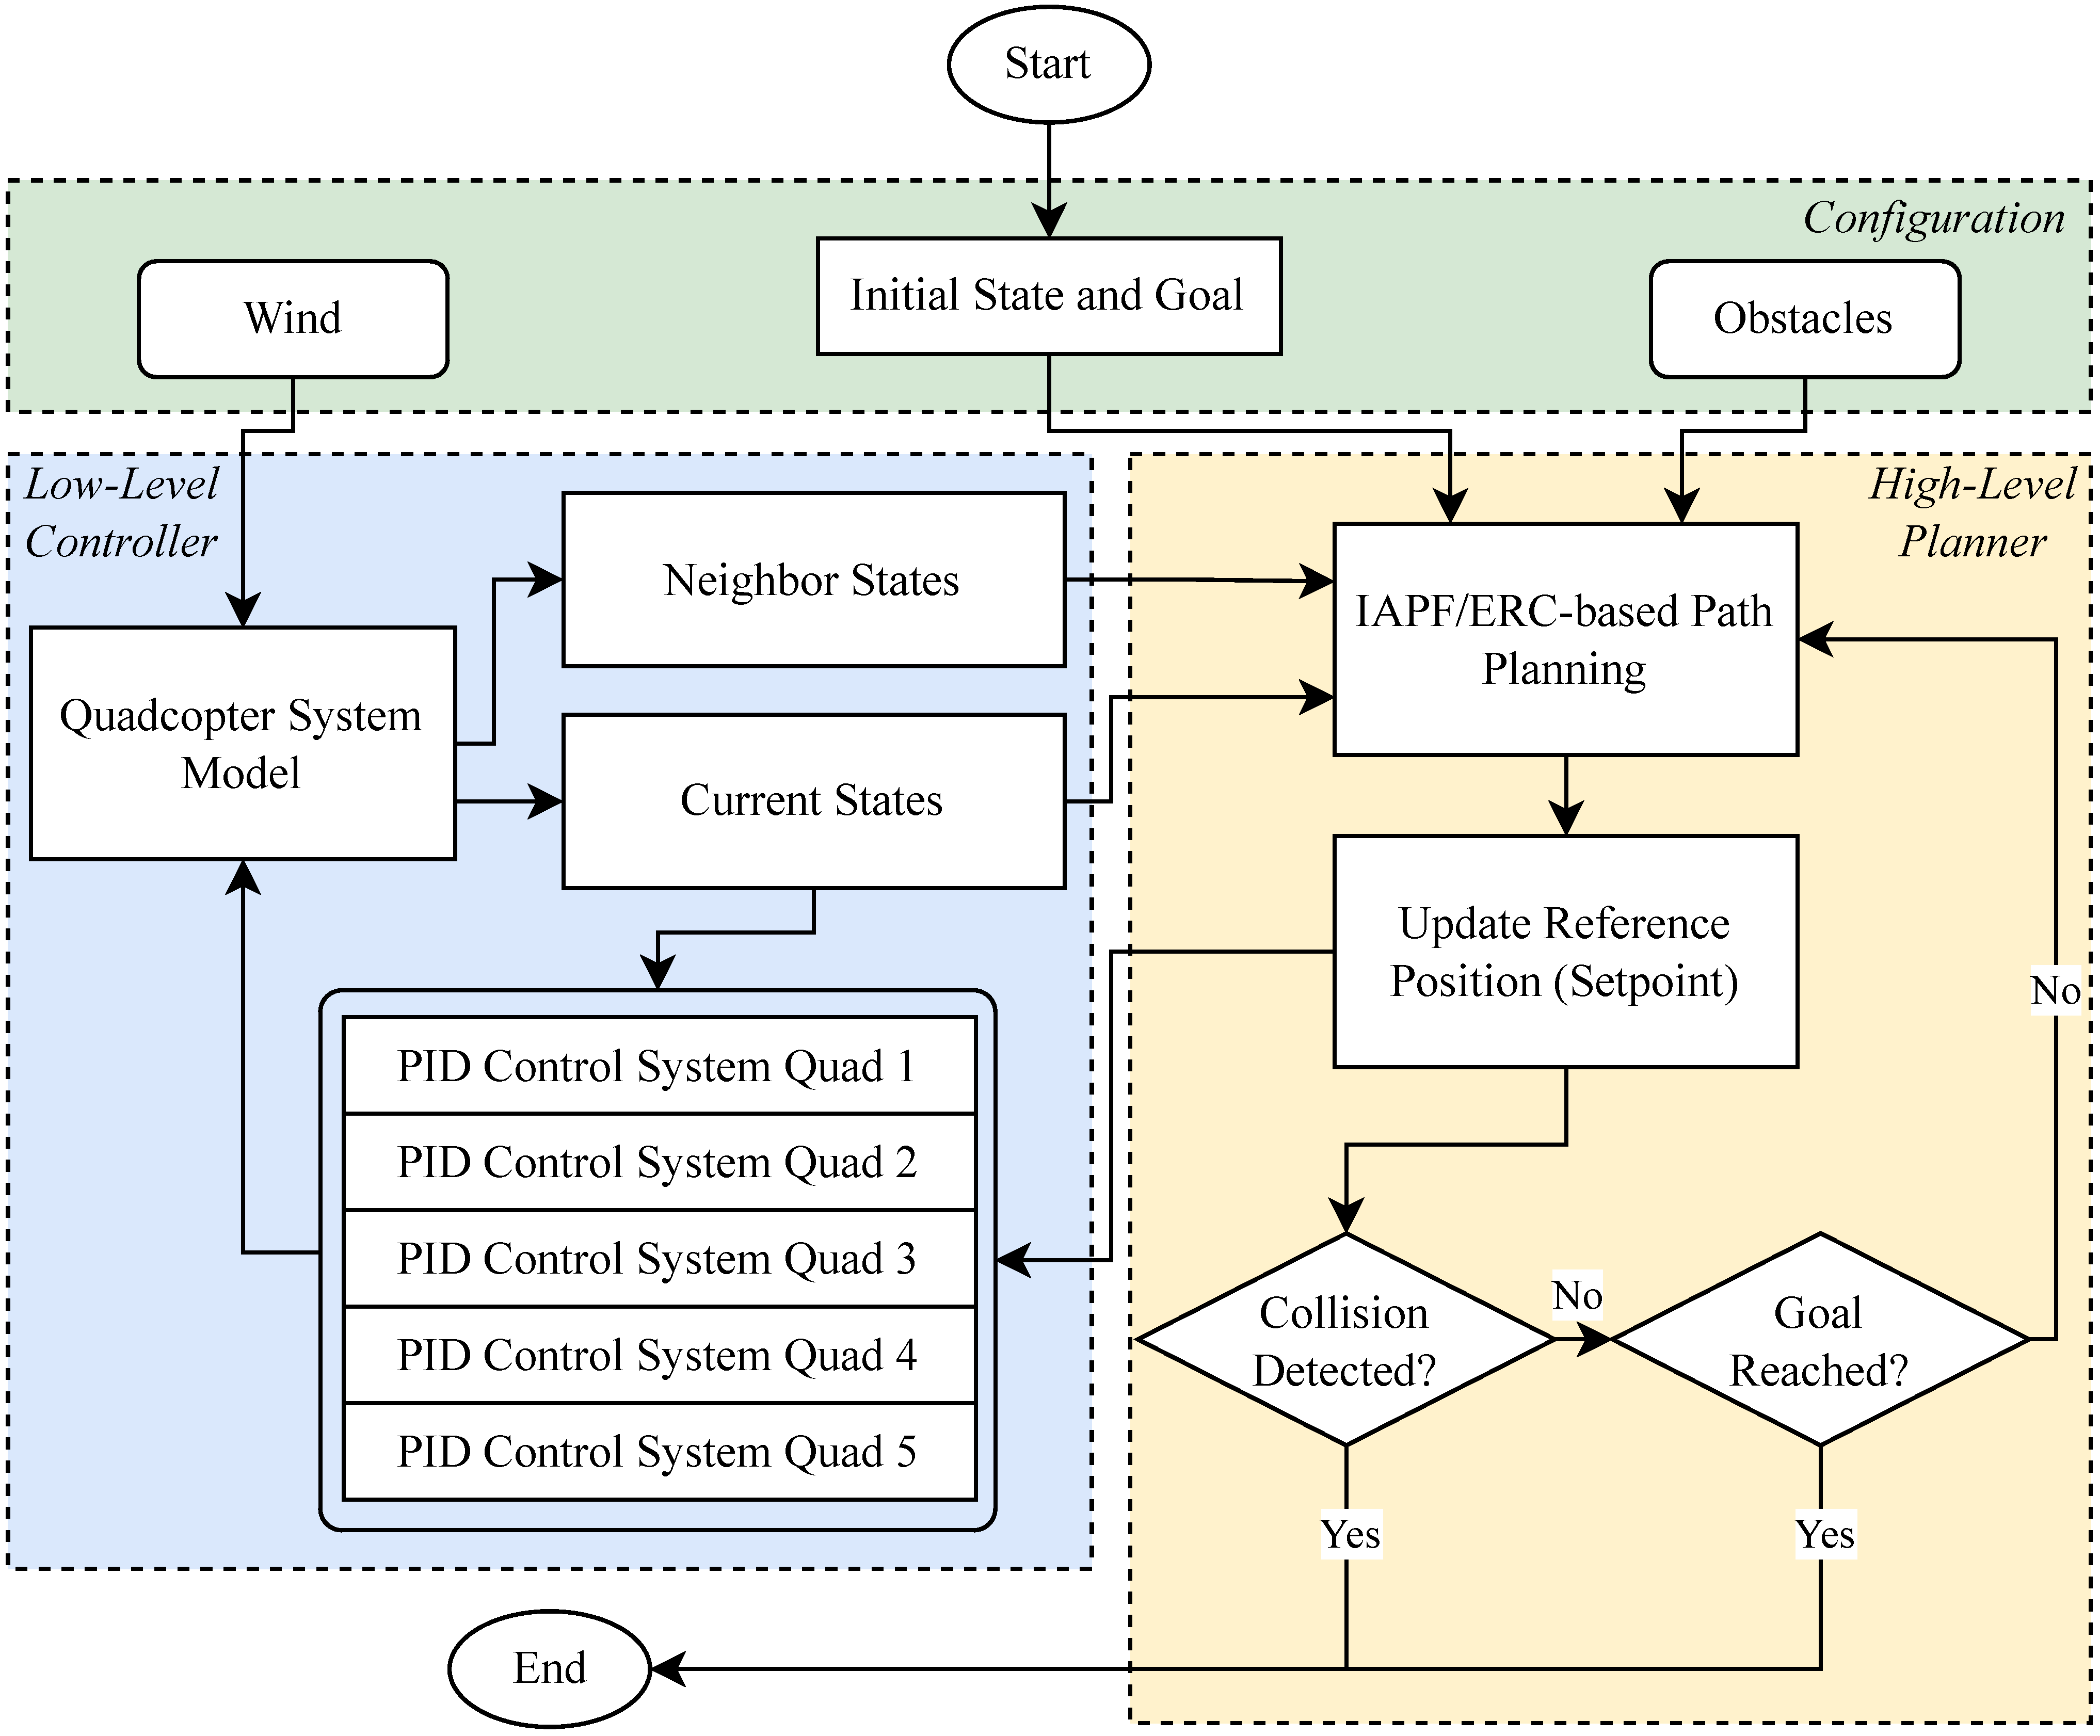
\includegraphics[width=0.75\columnwidth]{figures/architecture.pdf}
        \caption{The hierarchical control architecture, illustrating the information flow between the configuration, the high-level swarm planner, and the decentralized low-level controllers for each quadcopter.}
        \label{fig:architecture}
    \end{figure}

    The physical behavior of each quadcopter is represented by a white-box dynamic model derived using Kane's Method \citep{dimaggio_dynamics_1986, john_bobzwikquadcopter_simcon_2025}. Before establishing the complete mathematical model, it is necessary to define the primary reference frames and kinematic variables. The model is formulated with respect to a north-east-down (NED) inertial frame, where the vehicle's position is denoted by $(x,y,z)$, and its orientation is represented by the attitude quaternion $(q_w,q_x,q_y,q_z)$. A front-right-down (FRD) body frame is attached to the quadcopter's center of mass, where the body roll, pitch, and yaw rates are denoted by $\omega_{\phi}, \omega_{\theta}$, and $\omega_{\psi}$, respectively. The motion of the quadcopter is primarily driven by the thrust $T_{Mi}$ and the reaction torque $\tau_{Mi}$ generated by each individual rotor $i \in \{1,2,3,4\}$. A free-body diagram illustrating these coordinate frames and principal forces is shown in Fig.~\ref{fig:free_body_diagram}.

    \begin{figure}
        \centering
        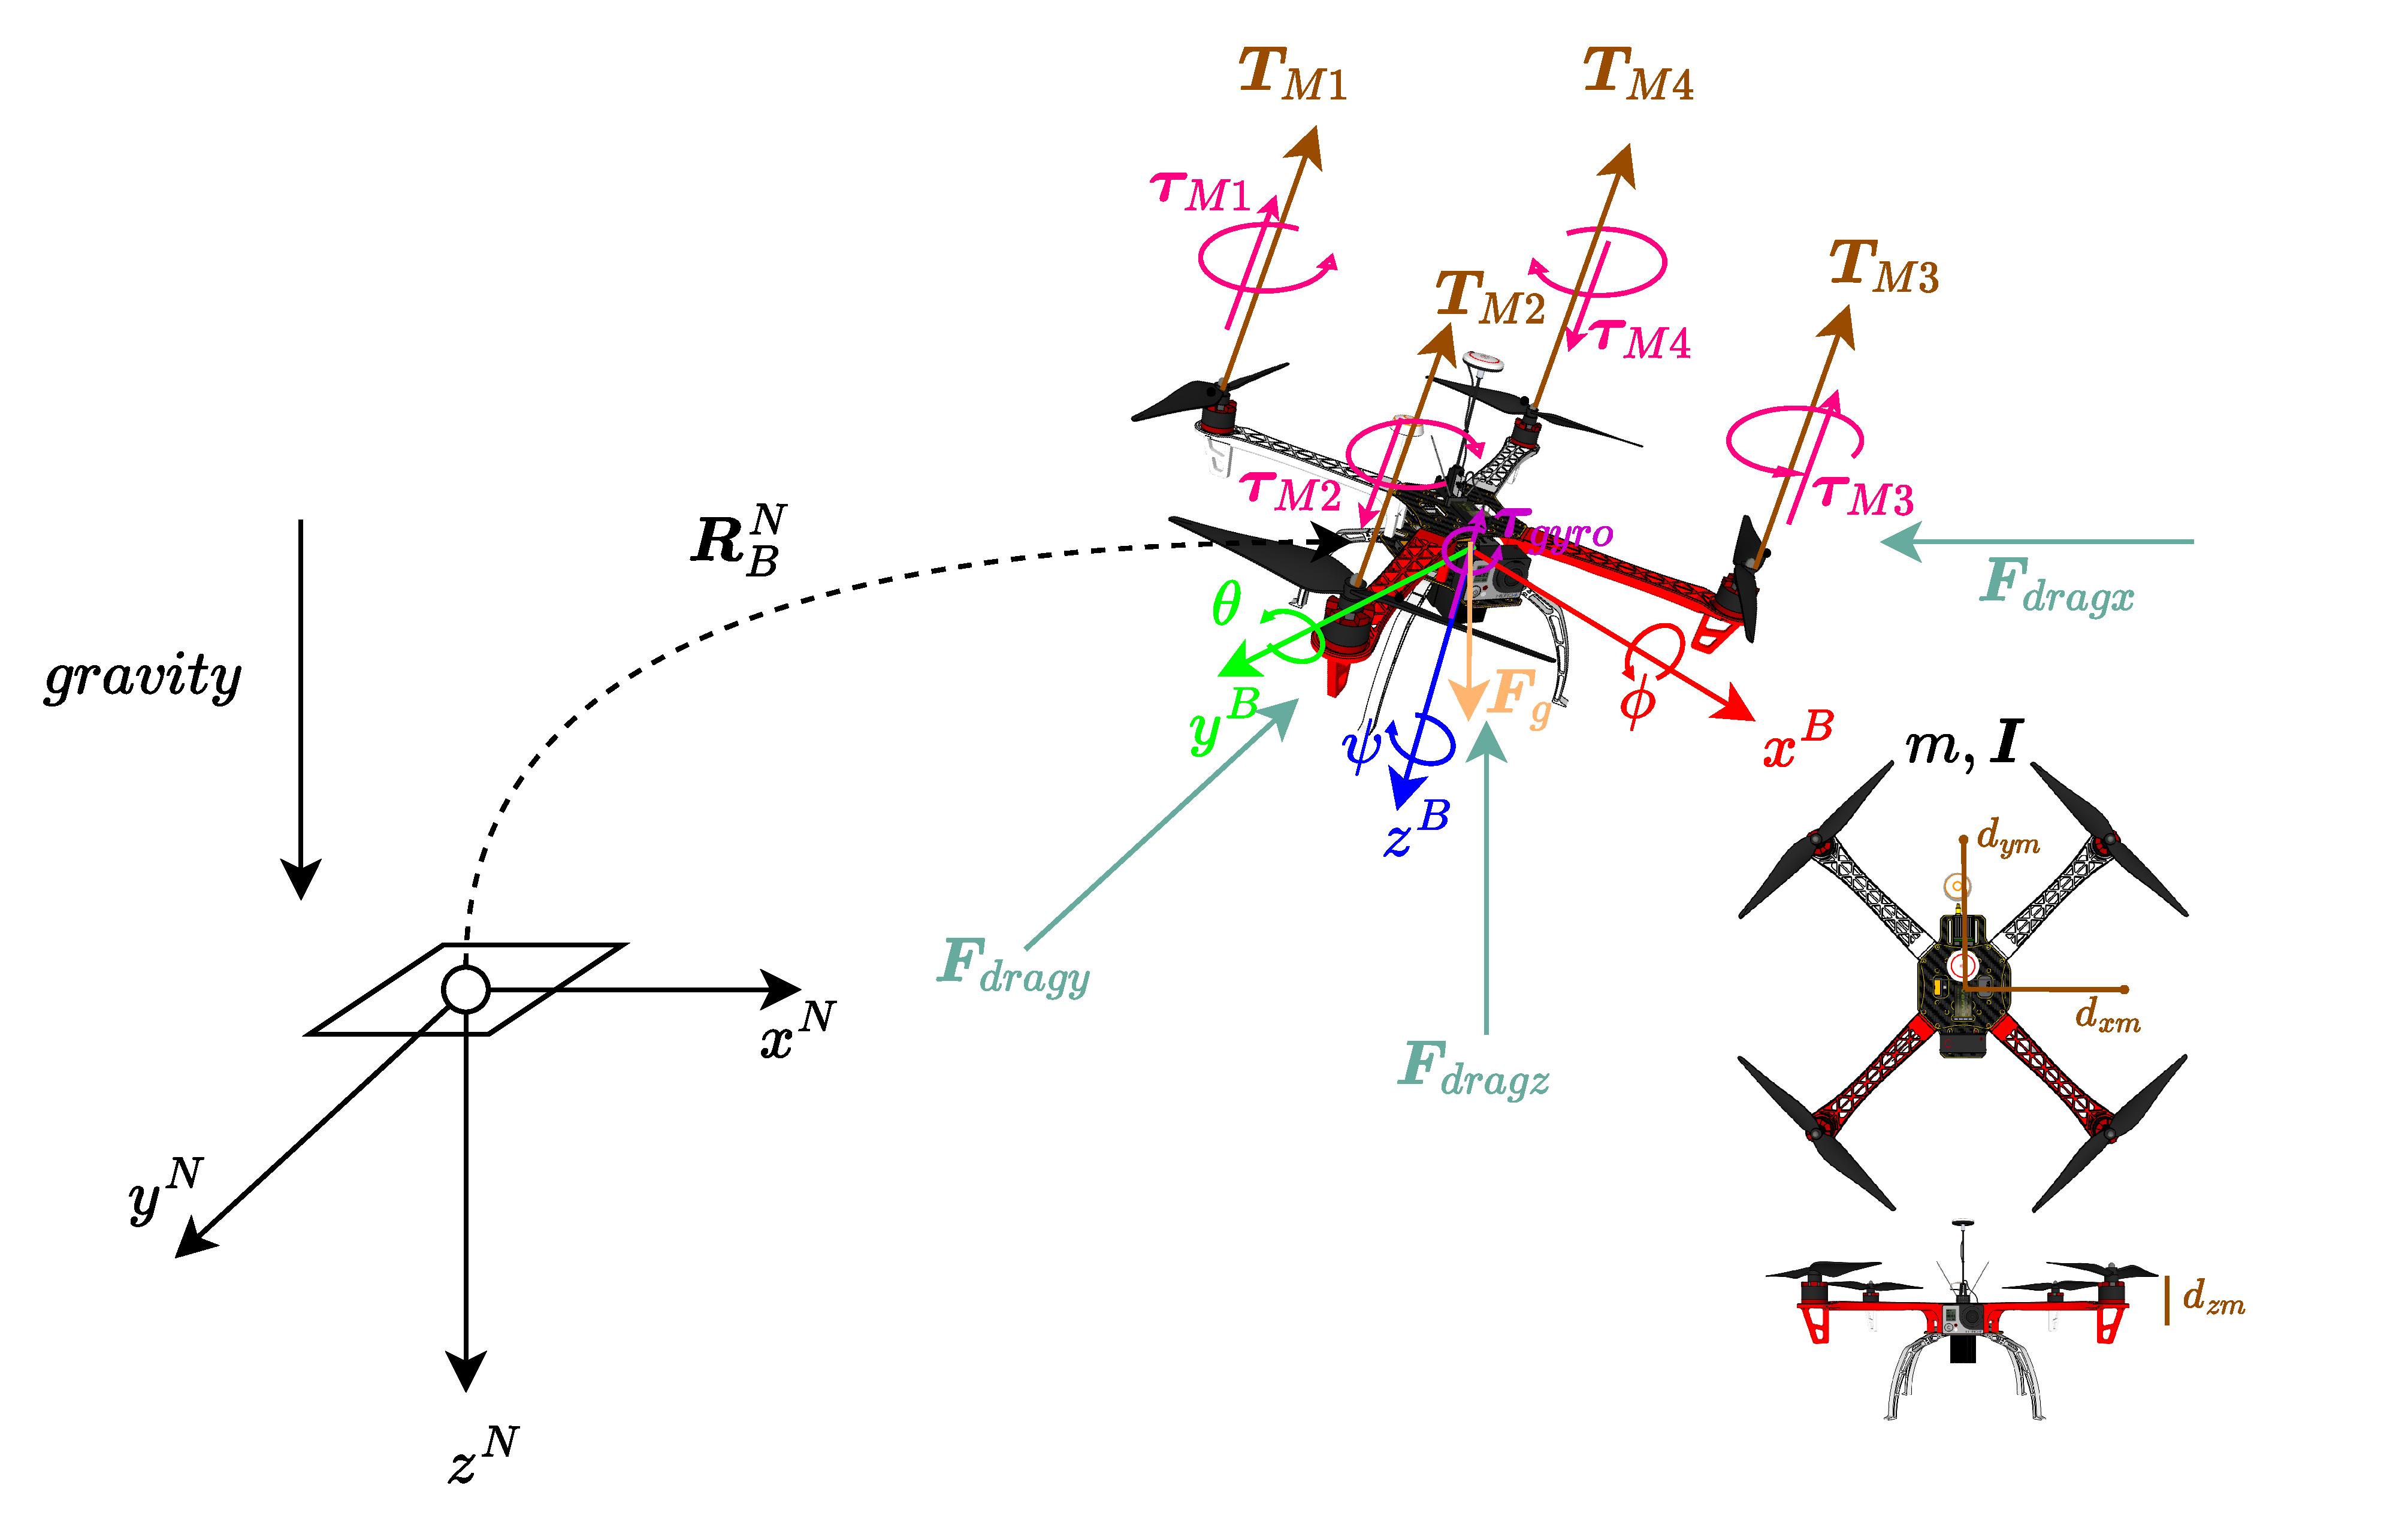
\includegraphics[width=0.75\columnwidth]{figures/free_body_diagram.pdf}
        \caption{Free-body diagram of the quadcopter illustrating the NED inertial frame, the FRD body frame, and the primary forces and torques acting on the system.}
        \label{fig:free_body_diagram}
    \end{figure}

    Building upon these kinematics, the complete nonlinear equations of motion describe the vehicle as a 6-DoF rigid body based on the inertial properties of a DJI F450 frame. The vehicle's mass is defined as $m_B$, while its principal moments of inertia along the body axes are $I_{Bxx}, I_{Byy}$, and $I_{Bzz}$. The rotor inertia is denoted by $I_{Rzz}$, and the orthogonal distances from the center of mass to the motors are $d_{xm}$ and $d_{ym}$. The model also accounts for external environmental factors: $C_d$ represents the aerodynamic drag coefficient, while $v_w$ and $(q_{w1}, q_{w2})$ represent the wind speed magnitude and its directional angles, respectively. A configuration constant $u_p \in \{-1, +1\}$ is used to determine the alternating rotational direction of the propellers.

    Furthermore, the dynamic response of the DC motors is modeled as a second-order system to realistically represent actuator characteristics. This response is driven by the control input command $u_{Mi}$ and is characterized by the motor static gain $k_p$, time constant $\xi$, and damping ratio $\zeta$. Integrating both the physical states of the rigid body and the actuator states ($\omega_{Mi}, \dot{\omega}_{Mi}$) forms a comprehensive 21-element state vector, $\mathbf{s}$. The resulting state-space representation of the quadcopter dynamics is formulated in Eq.~(\ref{eq:state_space}).

    \begingroup
    \small
    \setlength{\jot}{4pt}
    \begin{subequations}\label{eq:state_space}
    \makebox[\textwidth][c]{%
        \begin{minipage}{1.3\textwidth}
            \begin{align}
                \dot{\mathbf{s}} &= [
                \dot{x},\dot{y},\dot{z},\dot{q}_w,\dot{q}_x,\dot{q}_y,\dot{q}_z,
                \ddot{x},\ddot{y},\ddot{z},
                \dot{\omega}_{\phi},\dot{\omega}_{\theta},\dot{\omega}_{\psi},
                \dot{\omega}_{M1},\ddot{\omega}_{M1},
                \dot{\omega}_{M2},\ddot{\omega}_{M2},
                \dot{\omega}_{M3},\ddot{\omega}_{M3},
                \dot{\omega}_{M4},\ddot{\omega}_{M4}]^{\top}
                \label{eq:state_space_a} \\
                \dot{q}_w &= -0.5(\omega_\phi q_x + \omega_\theta q_y + \omega_\psi q_z) \\
                \dot{q}_x &= 0.5(\omega_\phi q_w - \omega_\theta q_z + \omega_\psi q_y) \\
                \dot{q}_y &= 0.5(\omega_\phi q_z + \omega_\theta q_w - \omega_\psi q_x) \\
                \dot{q}_z &= -0.5(\omega_\phi q_y - \omega_\theta q_x - \omega_\psi q_w)
                \label{eq:state_space_b} \\
                \ddot{x} &= \dfrac{C_d \, \mathrm{sign}(v_w \cos q_{w1} \cos q_{w2} - \dot{x})\left(v_w \cos q_{w1} \cos q_{w2} - \dot{x}\right)^2 - 2(q_w q_y + q_x q_z)(\sum T_{Mi})}{m_B} \\
                \ddot{y} &= \dfrac{C_d \, \mathrm{sign}(v_w \sin q_{w1} \cos q_{w2} - \dot{y})\left(v_w \sin q_{w1} \cos q_{w2} - \dot{y}\right)^2 + 2(q_w q_x - q_y q_z)(\sum T_{Mi})}{m_B} \\
                \ddot{z} &= \dfrac{- C_d \, \mathrm{sign}(v_w \sin q_{w2} + \dot{z})\left(v_w \sin q_{w2} + \dot{z}\right)^2 - (q_w^2 - q_x^2 - q_y^2 + q_z^2)(\sum T_{Mi}) + g m_B}{m_B}
                \label{eq:state_space_c} \\
                \dot{\omega}_{\phi} &= \dfrac{(I_{Byy} - I_{Bzz})\omega_\theta \omega_\psi - u_p I_{Rzz}(\omega_{M1} - \omega_{M2} + \omega_{M3} - \omega_{M4})\omega_\theta + (T_{M1} - T_{M2} - T_{M3} + T_{M4})d_{ym}}{I_{Bxx}} \\
                \dot{\omega}_{\theta} &= \dfrac{(I_{Bzz} - I_{Bxx})\omega_\phi \omega_\psi + u_p I_{Rzz}(\omega_{M1} - \omega_{M2} + \omega_{M3} - \omega_{M4})\omega_\phi + (T_{M1} + T_{M2} - T_{M3} - T_{M4})d_{xm}}{I_{Byy}} \\
                \dot{\omega}_{\psi} &= \dfrac{(I_{Bxx} - I_{Byy})\omega_\phi \omega_\theta + \tau_{M1} - \tau_{M2} + \tau_{M3} - \tau_{M4}}{I_{Bzz}}
                \label{eq:state_space_d} \\
                \ddot{\omega}_{Mi} &= \dfrac{-2\zeta\xi\dot{\omega}_{Mi} - \omega_{Mi} + k_p u_{Mi}}{\xi^2}, \qquad i\in\{1,2,3,4\}
            \label{eq:state_space_e}
            \end{align}
        \end{minipage}%
    }
    \end{subequations}
    \endgroup

    For the stabilization of individual agents, a cascaded proportional-integral-derivative (PID) control architecture is utilized \citep{john_bobzwikquadcopter_simcon_2025}. This multi-loop structure is responsible for translating the abstract position setpoints from the high-level planner into concrete motor commands. As depicted in the signal flow diagram in Fig.~\ref{fig:low_level_controller}, the High-Level Planner provides the reference position ($x_{\mathrm{ref}}, y_{\mathrm{ref}}, z_{\mathrm{ref}}$), feedforward reference acceleration ($a_{x\mathrm{ref}}, a_{y\mathrm{ref}}, a_{z\mathrm{ref}}$), as well as reference yaw and yaw rate ($\psi_{\mathrm{ref}}$ and $\dot{\psi}_{\mathrm{ref}}$).

    The control process begins in the outer translation loops. First, the Position P Controller computes the reference velocities ($v_{x\mathrm{ref}}, v_{y\mathrm{ref}}, v_{z\mathrm{ref}}$) based on the position tracking error. Next, the Velocity PID Controller takes these computed reference velocities, the current measured velocities, and the feedforward reference accelerations to calculate the required directional thrust components ($T_x, T_y, T_z$).

    These thrust components are then passed to the Thrust to Attitude block. Using the directional thrusts and the reference yaw ($\psi_{\mathrm{ref}}$), this block computes the scalar total thrust $T = \sqrt{T_x^2 + T_y^2 + T_z^2}$ (which is routed directly to the Mixer) and the target orientation quaternion ($q_{w\mathrm{des}}, q_{x\mathrm{des}}, q_{y\mathrm{des}}, q_{z\mathrm{des}}$).

    The inner rotational loops then track this desired orientation. The Attitude P Controller compares the target quaternion with the current measured attitude to output the desired angular rates ($\omega_{\phi\mathrm{des}}, \omega_{\theta\mathrm{des}}, \omega_{\psi\mathrm{des}}$). Subsequently, the Rate PD Controller uses these desired rates, the current angular rates, and the feedforward reference yaw rate ($\dot{\psi}_{\mathrm{ref}}$) to generate the final control torques ($\tau_{\phi}, \tau_{\theta}, \tau_{\psi}$). Ultimately, the Mixer block allocates the scalar total thrust $T$ and the control torques to deduce the specific control signals ($u_{M1}, u_{M2}, u_{M3}, u_{M4}$) required by the actuator dynamics.

    \begin{figure}
        \centering
        \makebox[\linewidth][c]{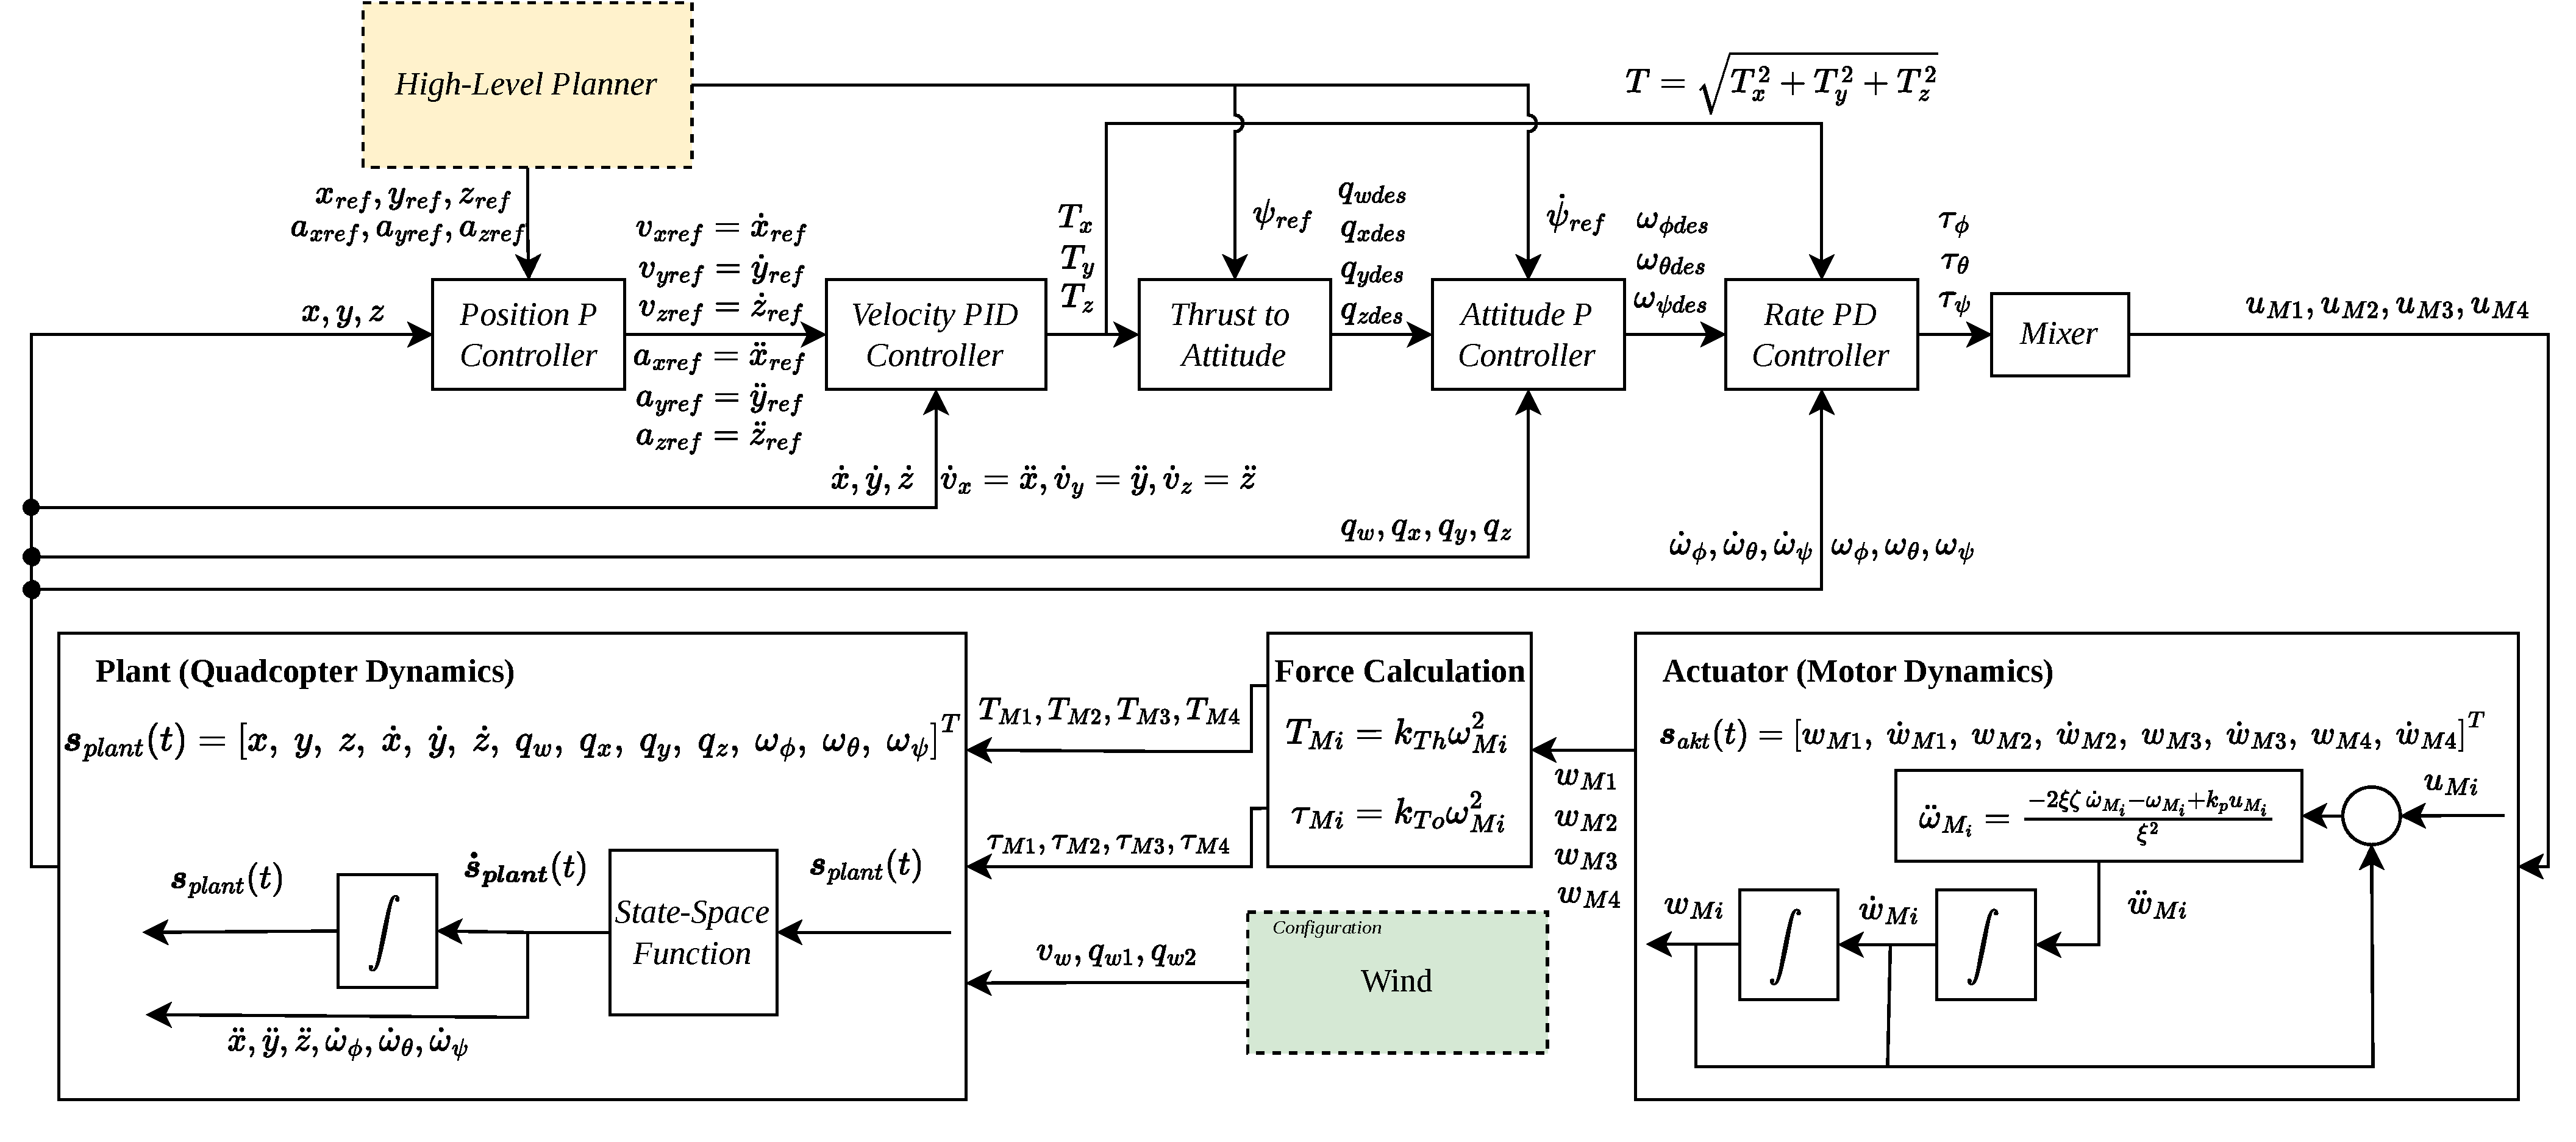
\includegraphics[width=1.2\linewidth]{figures/low_level_controller.pdf}}
        \caption{Detailed architecture of the low-level controller, illustrating the cascaded control loops from position setpoint to motor command allocation.}
        \label{fig:low_level_controller}
    \end{figure}

    While the low-level controller ensures the stability of each individual agent, the high-level planner is responsible for the intelligent, collective behavior of the entire swarm. The detailed design of this planner, which constitutes the core of our proposed formation control strategy, is presented in the following section.

\section{High-Level Planner: Decentralized and Adaptive Formation Control}
    The high-level planner serves as the collective intelligence of the swarm, responsible for generating the desired position setpoint ($\boldsymbol{p}_{\text{ref}}$) for each quadcopter in a decentralized manner. Its design is an adaptation and significant enhancement of the behavior-based framework proposed by Bui et al. \citep{bui_event-based_2025}, which integrates the Improved Artificial Potential Field (IAPF) and Event-based Reconfiguration Control (ERC) strategies. To effectively control a 3D quadcopter swarm, the foundational framework was enhanced with key functionalities, including a mission state machine, dynamic 3D goal navigation, and an adaptive formation orientation mechanism. The complete architecture of the proposed high-level planner is illustrated in Fig.~\ref{fig:high_level_planner}. The following subsections provide a detailed explanation of each component within this architecture.

    \begin{figure}
        \centering
        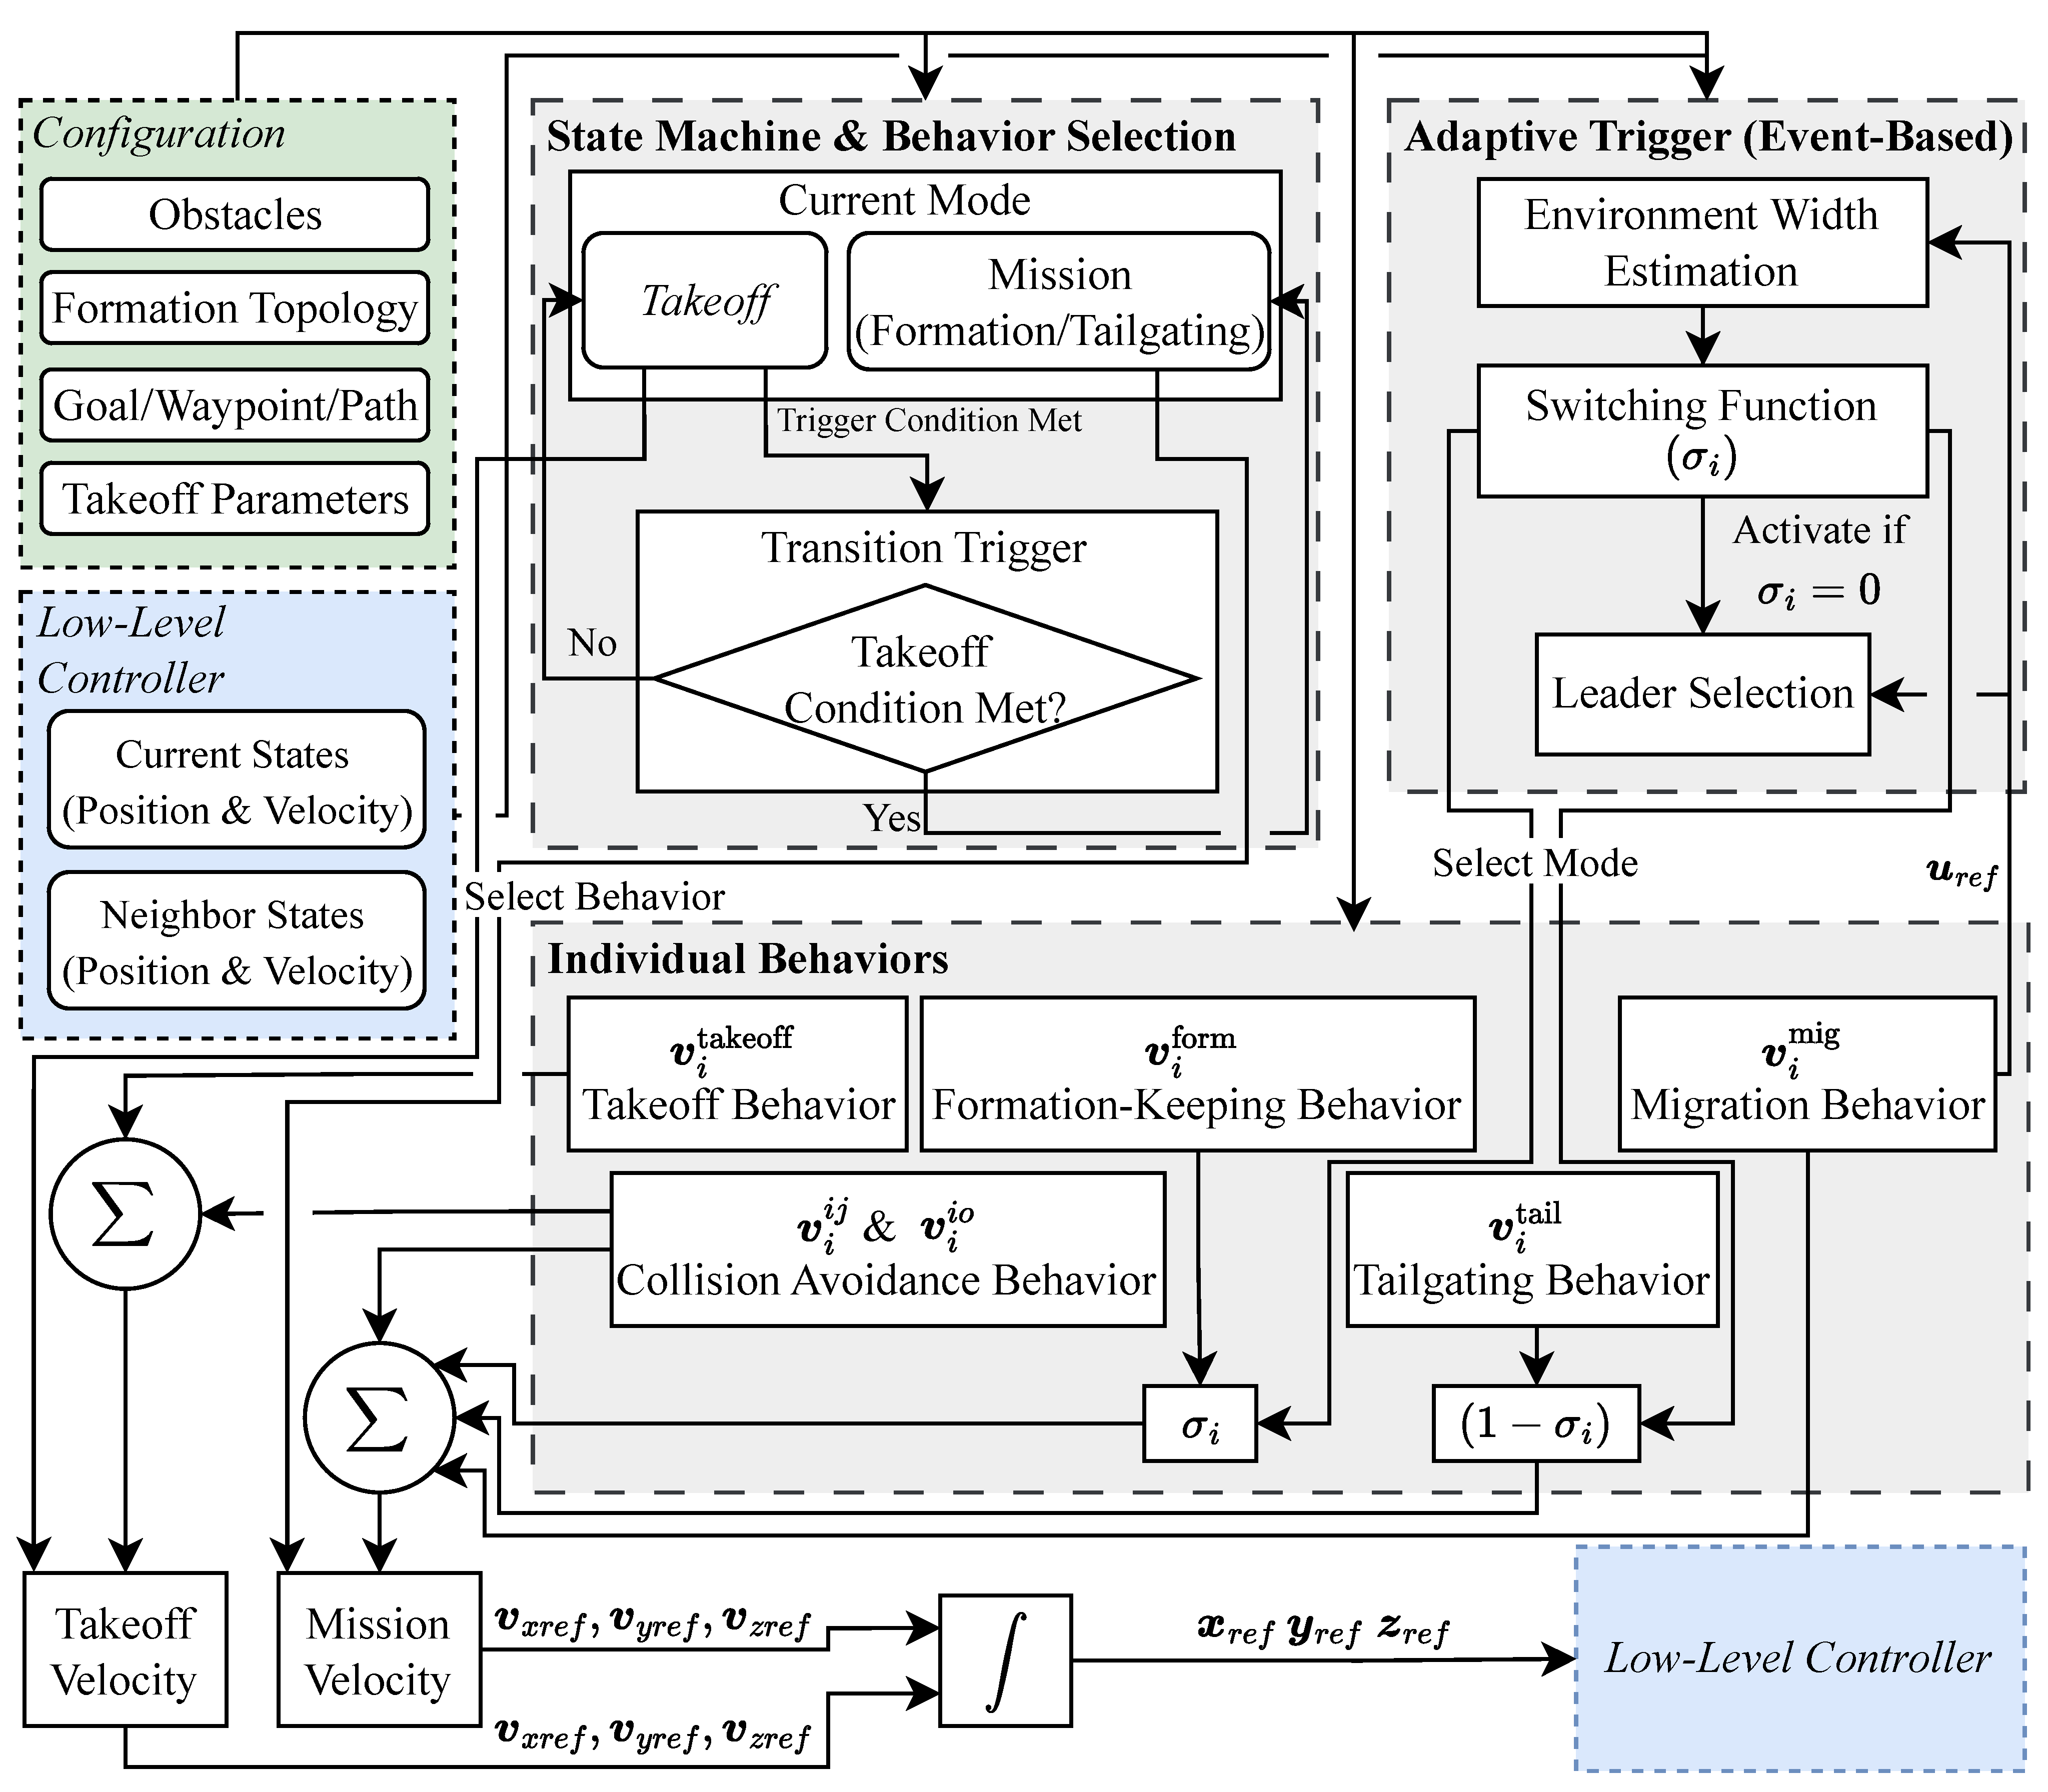
\includegraphics[width=0.9\textwidth]{figures/high_level_planner.pdf}
        \caption{Detailed architecture of the high-level planner, illustrating the interaction between configuration parameters, state machine logic, adaptive triggers, and individual behavior modules for mission execution.}
        \label{fig:high_level_planner}
    \end{figure}

    \subsection{State Machine and Mode Transition}
        The planner logic is governed by a state machine to ensure orderly mission execution and transitions between two primary modes: \textbf{takeoff} and \textbf{mission}. The takeoff mode is the initial phase in which all quadcopters ascend to a target altitude ($z_{\text{target}}$). During this phase, only the takeoff and collision-avoidance behaviors are active. A synchronous trigger initiates the transition to mission mode only when the vertical position of every quadcopter ($z_i$) is within a specified tolerance ($\epsilon_z$) of the target altitude, ensuring that the entire swarm is fully prepared before initiating formation navigation. This condition is formally expressed as:

        \begin{align}
            |z_{i}(t)-z_{\text{target}}| \le \epsilon_{z}, \quad \forall i\in\{1,...,N\}
        \end{align}

        Once this condition is met, the system enters mission mode, where all primary navigation and formation control behaviors are activated.

    \subsection{Formation Topology}
        The geometric arrangement of the swarm is defined by the desired formation topology. This is mathematically represented by a set of desired relative position vectors, $\boldsymbol{\delta}_{i}^{*} \in \mathbb{R}^{3}$, which dictates the ideal position of each agent and serves as the target configuration for the formation-keeping behavior. The two primary planar topologies utilized in this study are illustrated in Fig.~\ref{fig:topologies}.

        \begin{figure}
            \centering
            \begin{subfigure}[b]{0.48\columnwidth}
                \centering
                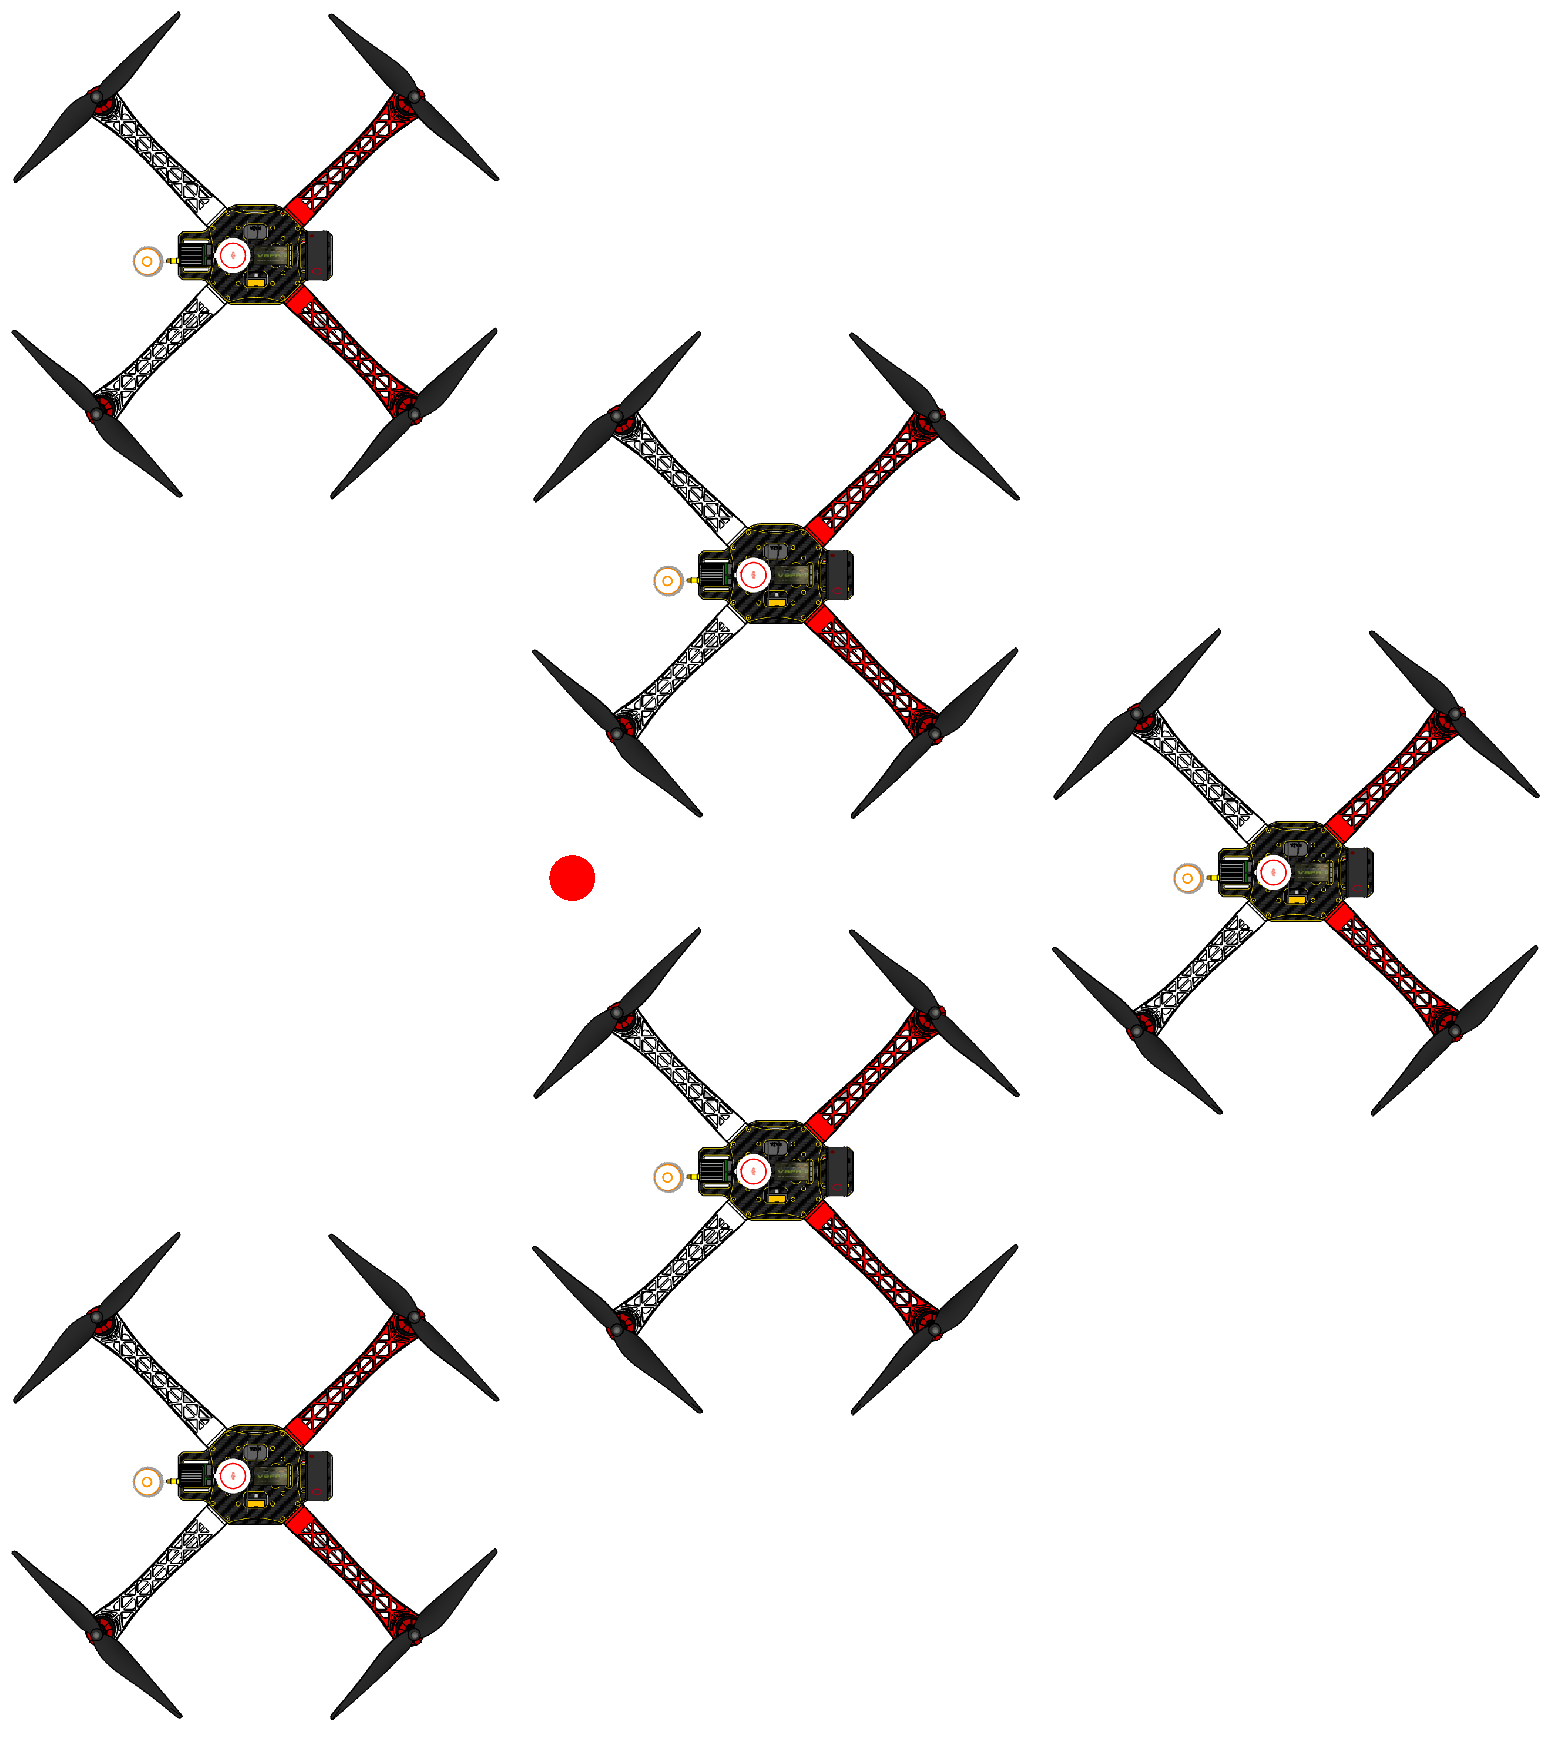
\includegraphics[width=0.8\linewidth]{figures/v_shape_topology.pdf}
                \caption{V-shape Topology}
                \label{fig:v_shape}
            \end{subfigure}
            \hfill
            \begin{subfigure}[b]{0.48\columnwidth}
                \centering
                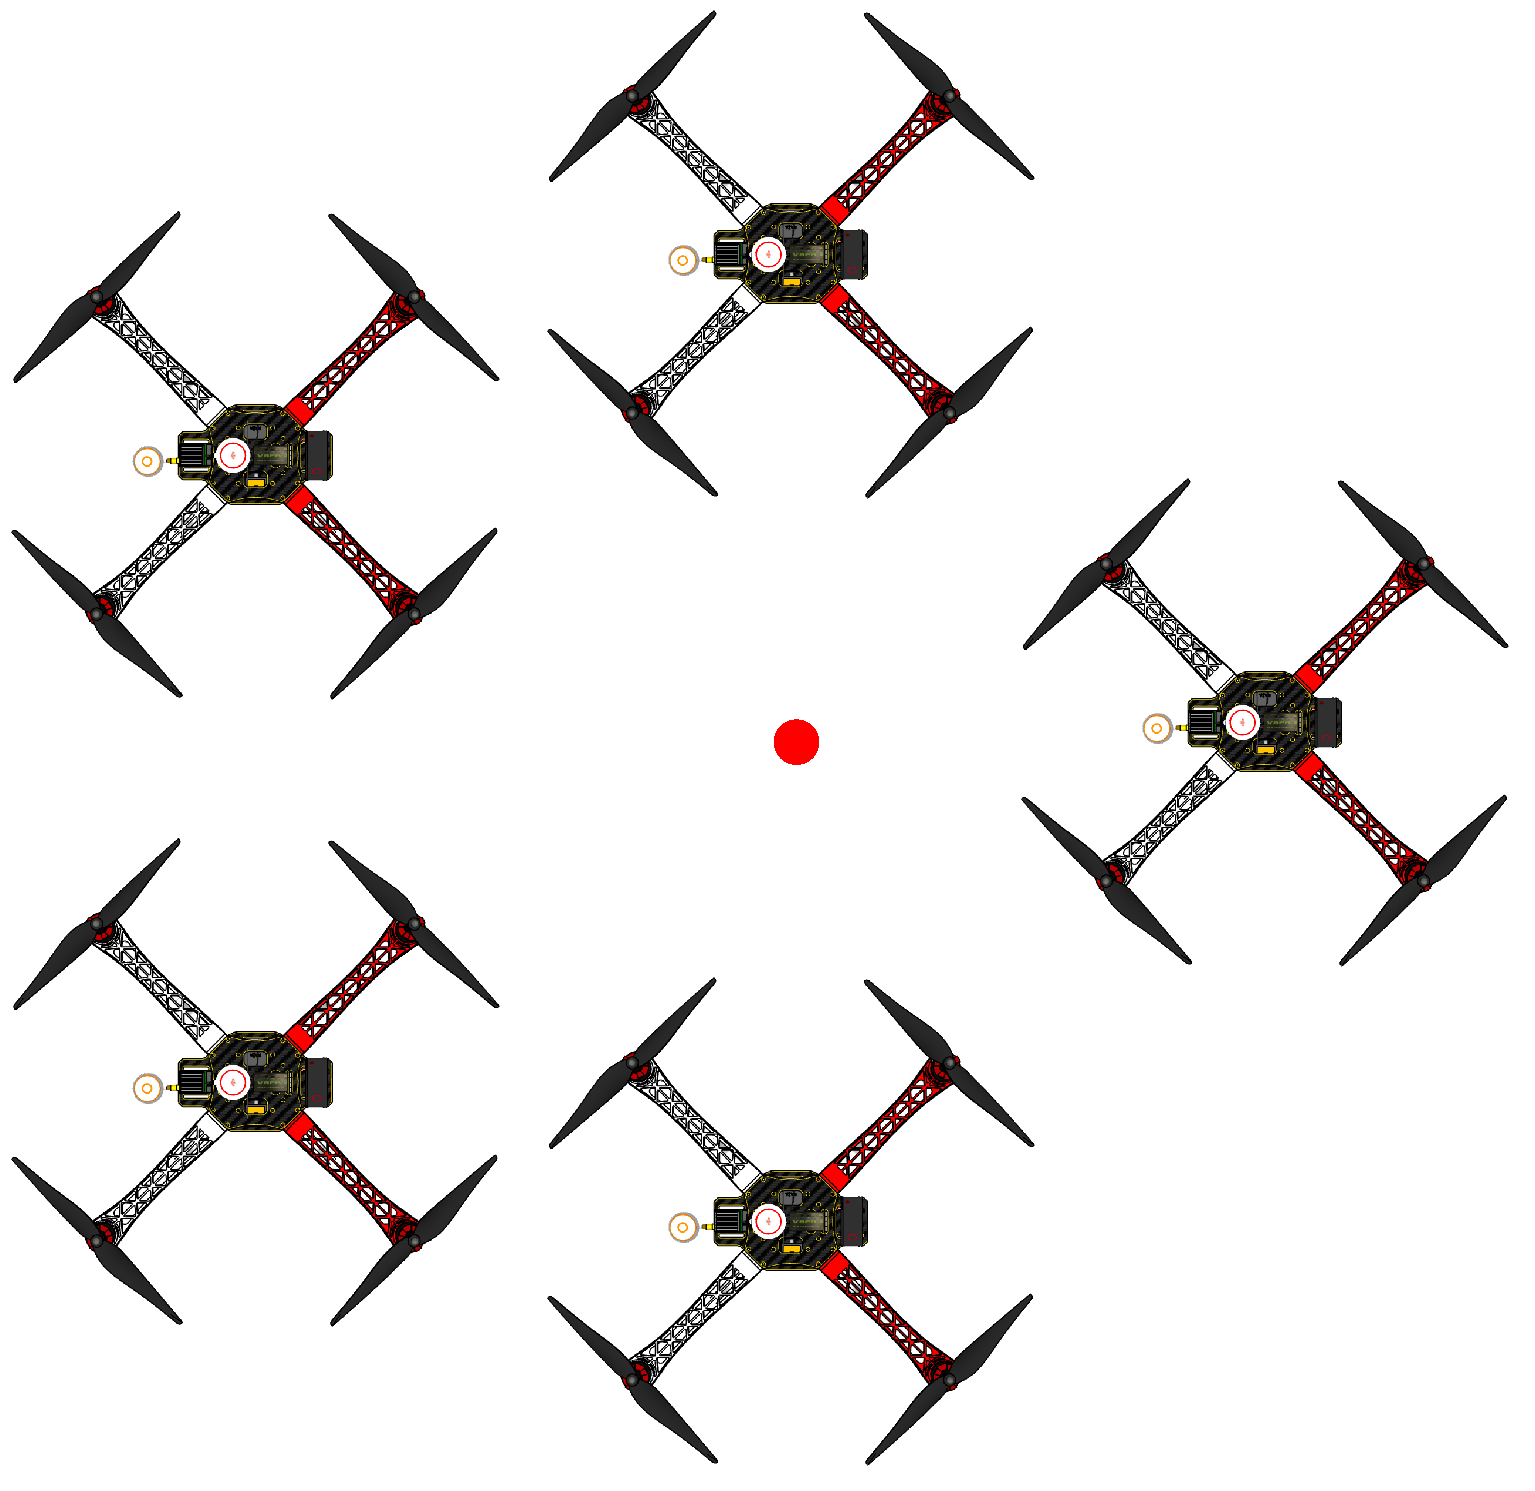
\includegraphics[width=0.8\linewidth]{figures/polygon_topology.pdf}
                \caption{Polygon Topology}
                \label{fig:polygon}
            \end{subfigure}
            \caption{The two primary formation topologies used: (a) V-shape and (b) Polygon.}
            \label{fig:topologies}
        \end{figure}

        \begin{itemize}
            \item \textbf{V-shape Formation:} As illustrated in Fig.~\ref{fig:v_shape}, this topology is explicitly defined for a five-agent swarm by the following set of vectors:
            \begin{equation}
            \label{eq:v_shape_matrix}
                \begin{bmatrix}
                    \boldsymbol{\delta}_{1}^{*} \\
                    \boldsymbol{\delta}_{2}^{*} \\
                    \boldsymbol{\delta}_{3}^{*} \\
                    \boldsymbol{\delta}_{4}^{*} \\
                    \boldsymbol{\delta}_{5}^{*}
                \end{bmatrix}
                =
                \begin{bmatrix}
                    1.0 & 0.0 & 0.0 \\
                    -1.0 & 1.0 & 0.0 \\
                    0.0 & 0.5 & 0.0 \\
                    0.0 & -0.5 & 0.0 \\
                    -1.0 & -1.0 & 0.0
                \end{bmatrix}
            \end{equation}

            \item \textbf{Polygon Formation:} This topology, depicted in Fig.~\ref{fig:polygon}, arranges the $N$ agents of the swarm evenly on the circumference of a circle to form a regular polygon. The desired position vector for agent $i$ is determined by the equation:
            \begin{equation}
                \boldsymbol{\delta}_{i}^{*} = \begin{bmatrix} \cos(2\pi i/N) & \sin(2\pi i/N) & 0 \end{bmatrix}^T
            \end{equation}
        \end{itemize}

    \subsection{Core Behavioral Components}
        The foundational logic of the planner relies on several behavioral components adapted from the established reactive literature \citep{bui_event-based_2025}. In this hierarchical control framework, the output of each behavior generates a desired spatial velocity vector. The primary behaviors are formulated as follows:

        \begin{itemize}
            \item \textbf{Formation-Keeping Behavior ($\boldsymbol{v}_i^{\text{form}}$):} As illustrated in Fig.~\ref{fig:behavior_formation}, this component guides each quadcopter toward its ideal coordinate within the predefined topology. The vector is governed by a scaling gain $k_{\text{form}}$ and a dynamic formation scaling factor $\kappa$:
            \begin{equation}
                \boldsymbol{v}_{i}^{\text{form}} = k_{\text{form}}\sum_{j=1,j\ne i}^{N}((\boldsymbol{p}_{j}-\boldsymbol{p}_{i})-\kappa(\boldsymbol{\delta}_{j}^{*}-\boldsymbol{\delta}_{i}^{*}))
            \end{equation}

            \item \textbf{Migration Behavior ($\boldsymbol{v}_i^{\text{mig}}$):} Depicted in Fig.~\ref{fig:behavior_migration}, this behavior directs the swarm toward a common goal direction, represented by the unit vector $\boldsymbol{u}_{\text{ref}}$, at a reference cruise speed, $v_{\text{ref}}$:
            \begin{align}
                \boldsymbol{v}_{i}^{\text{mig}} = v_{\text{ref}} \boldsymbol{u}_{\text{ref}}
            \end{align}
            
            \item \textbf{Collision Avoidance Behavior ($\boldsymbol{v}_i^{\text{rep}}$):} Illustrated in Fig.~\ref{fig:behavior_avoidance}, this repulsive component prevents collisions by computing velocities directed away from neighboring agents ($\boldsymbol{v}_{i}^{ij}$) and static obstacles ($\boldsymbol{v}_{i}^{io}$). It activates strictly when an object breaches the predefined safety radius $r_a$, with repulsion strengths scaled by $k_{\text{col}}$ and $k_{\text{obs}}$:
            \begin{align}
                \boldsymbol{v}_{i}^{ij} &= k_{\text{col}}\left(\frac{1}{||\boldsymbol{p}_{ij}||}-\frac{1}{r_{a}}\right)\frac{1}{||\boldsymbol{p}_{ij}||^{2}}\boldsymbol{\hat{p}}_{ij}+\boldsymbol{v}_{j} \\
                \boldsymbol{v}_{i}^{io} &= k_{\text{obs}}\left(\frac{1}{||\boldsymbol{p}_{io}||}-\frac{1}{r_{a}}\right)\frac{1}{||\boldsymbol{p}_{io}||^{2}}\boldsymbol{\hat{p}}_{io}
            \end{align}

            \item \textbf{Tailgating Behavior ($\boldsymbol{v}_i^{\text{tail}}$):} Shown in Fig.~\ref{fig:behavior_tailgating}, this mode is crucial for traversing narrow corridors. It compels a follower quadcopter ($\boldsymbol{p}_i$) to track its designated leader ($\boldsymbol{p}_{li}$) while rigidly maintaining a safe reference distance ($d_{\text{ref}}$) weighted by $k_{\text{tail}}$:
            \begin{equation}
                \boldsymbol{v}_{i}^{\text{tail}} = k_{\text{tail}}\left((\boldsymbol{p}_{li}-\boldsymbol{p}_{i})-d_{\text{ref}}\frac{\boldsymbol{v}_{li}}{||\boldsymbol{v}_{li}||}\right)+\boldsymbol{v}_{li}
            \end{equation}
            Unlike traditional leader-follower frameworks that mandate both positional and orientational tracking, this formulation intentionally governs only positional separation. Because quadcopters are horizontally holonomic, the individual heading ($\psi_i$) is dynamically decoupled and globally aligned with the formation's migration direction ($\psi_{\text{form}}$), as detailed in next Section. Restricting the tailgating control exclusively to translational kinematics eliminates unnecessary yaw maneuvering. This specific design choice prevents cross-coupling oscillations between the rotational and translational dynamic loops, thereby significantly enhancing the attitude stability and aerodynamic robustness of the followers during high-speed corridor traversal.
        \end{itemize}

    \subsection{Enhancements for 3D Quadcopter Swarm}
        To elevate the baseline 2D planar framework into a fully operational 3D aerial system, the following critical functionalities were integrated:

        \begin{itemize}
            \item \textbf{Takeoff Behavior ($\boldsymbol{v}_i^{\text{takeoff}}$):} Depicted in Fig.~\ref{fig:behavior_takeoff}, this behavior regulates the initial ascent. It generates a strictly vertical velocity vector to ensure synchronous elevation. The target vertical speed, $v_{z,\text{des}}^{\text{takeoff}}$, is computed via a proportional controller based on the altitude error:
            \begin{align}
                v_{z,\text{des}}^{\text{takeoff}} &= k_{p,\text{takeoff}}(z_{\text{target}} - z_i(t)) \\
                \boldsymbol{v}_{i}^{\text{takeoff}} &= \begin{bmatrix} 0 & 0 & v_{z,\text{des}}^{\text{takeoff}} \end{bmatrix}^T
            \end{align}

            \item \textbf{3D Goal Navigation:} The basic migration logic is expanded to support waypoint sequencing and continuous tracking. The global direction vector, $\boldsymbol{u}_{\text{ref}}$, is dynamically updated as the normalized vector spanning from the swarm's centroid ($\boldsymbol{p}_{\text{center}}$) to the current active goal ($\boldsymbol{p}_{\text{goal}}$):
            \begin{equation}
                \boldsymbol{u}_{\text{ref}}=\frac{\boldsymbol{p}_{\text{goal}}-\boldsymbol{p}_{\text{center}}}{||\boldsymbol{p}_{\text{goal}}-\boldsymbol{p}_{\text{center}}||}
            \end{equation}

            \item \textbf{Dynamic Formation Orientation and Individual Heading:} To emulate cohesive biological movement, the formation topology dynamically aligns with the flight path. The global formation yaw angle, $\psi_{\text{form}}$, is continuously extracted from the horizontal components of the migration directional vector $\boldsymbol{u}_{\text{ref}} = [u_x, u_y, u_z]^T$:
            \begin{equation}
                \psi_{\text{form}}=\text{atan2}(u_{y},u_{x})
            \end{equation}
            A 2D rotation matrix is subsequently applied to the base target vectors $\boldsymbol{\delta}_{i}^{*}$, ensuring the entire formation structure continuously "faces" the migration direction. Furthermore, to address the orientation of each specific agent within this framework, the individual yaw setpoint ($\psi_{i,\text{ref}}$) for all quadcopters is synchronously aligned with this formation heading ($\psi_{i,\text{ref}} = \psi_{\text{form}}$). Because a quadcopter is horizontally holonomic, the instantaneous positional velocities ($\boldsymbol{v}_{\text{ref}}$) generated by the collision avoidance and tailgating behaviors are actuated entirely through roll ($\phi$) and pitch ($\theta$) adjustments by the low-level controller. This decoupling ensures that the individual agents maintain a uniform forward-facing orientation toward the global goal, even when performing sudden lateral evasive maneuvers.
            
        \end{itemize}

        \begin{figure}
            \centering
            \begin{subfigure}[b]{0.32\textwidth}
                \centering
                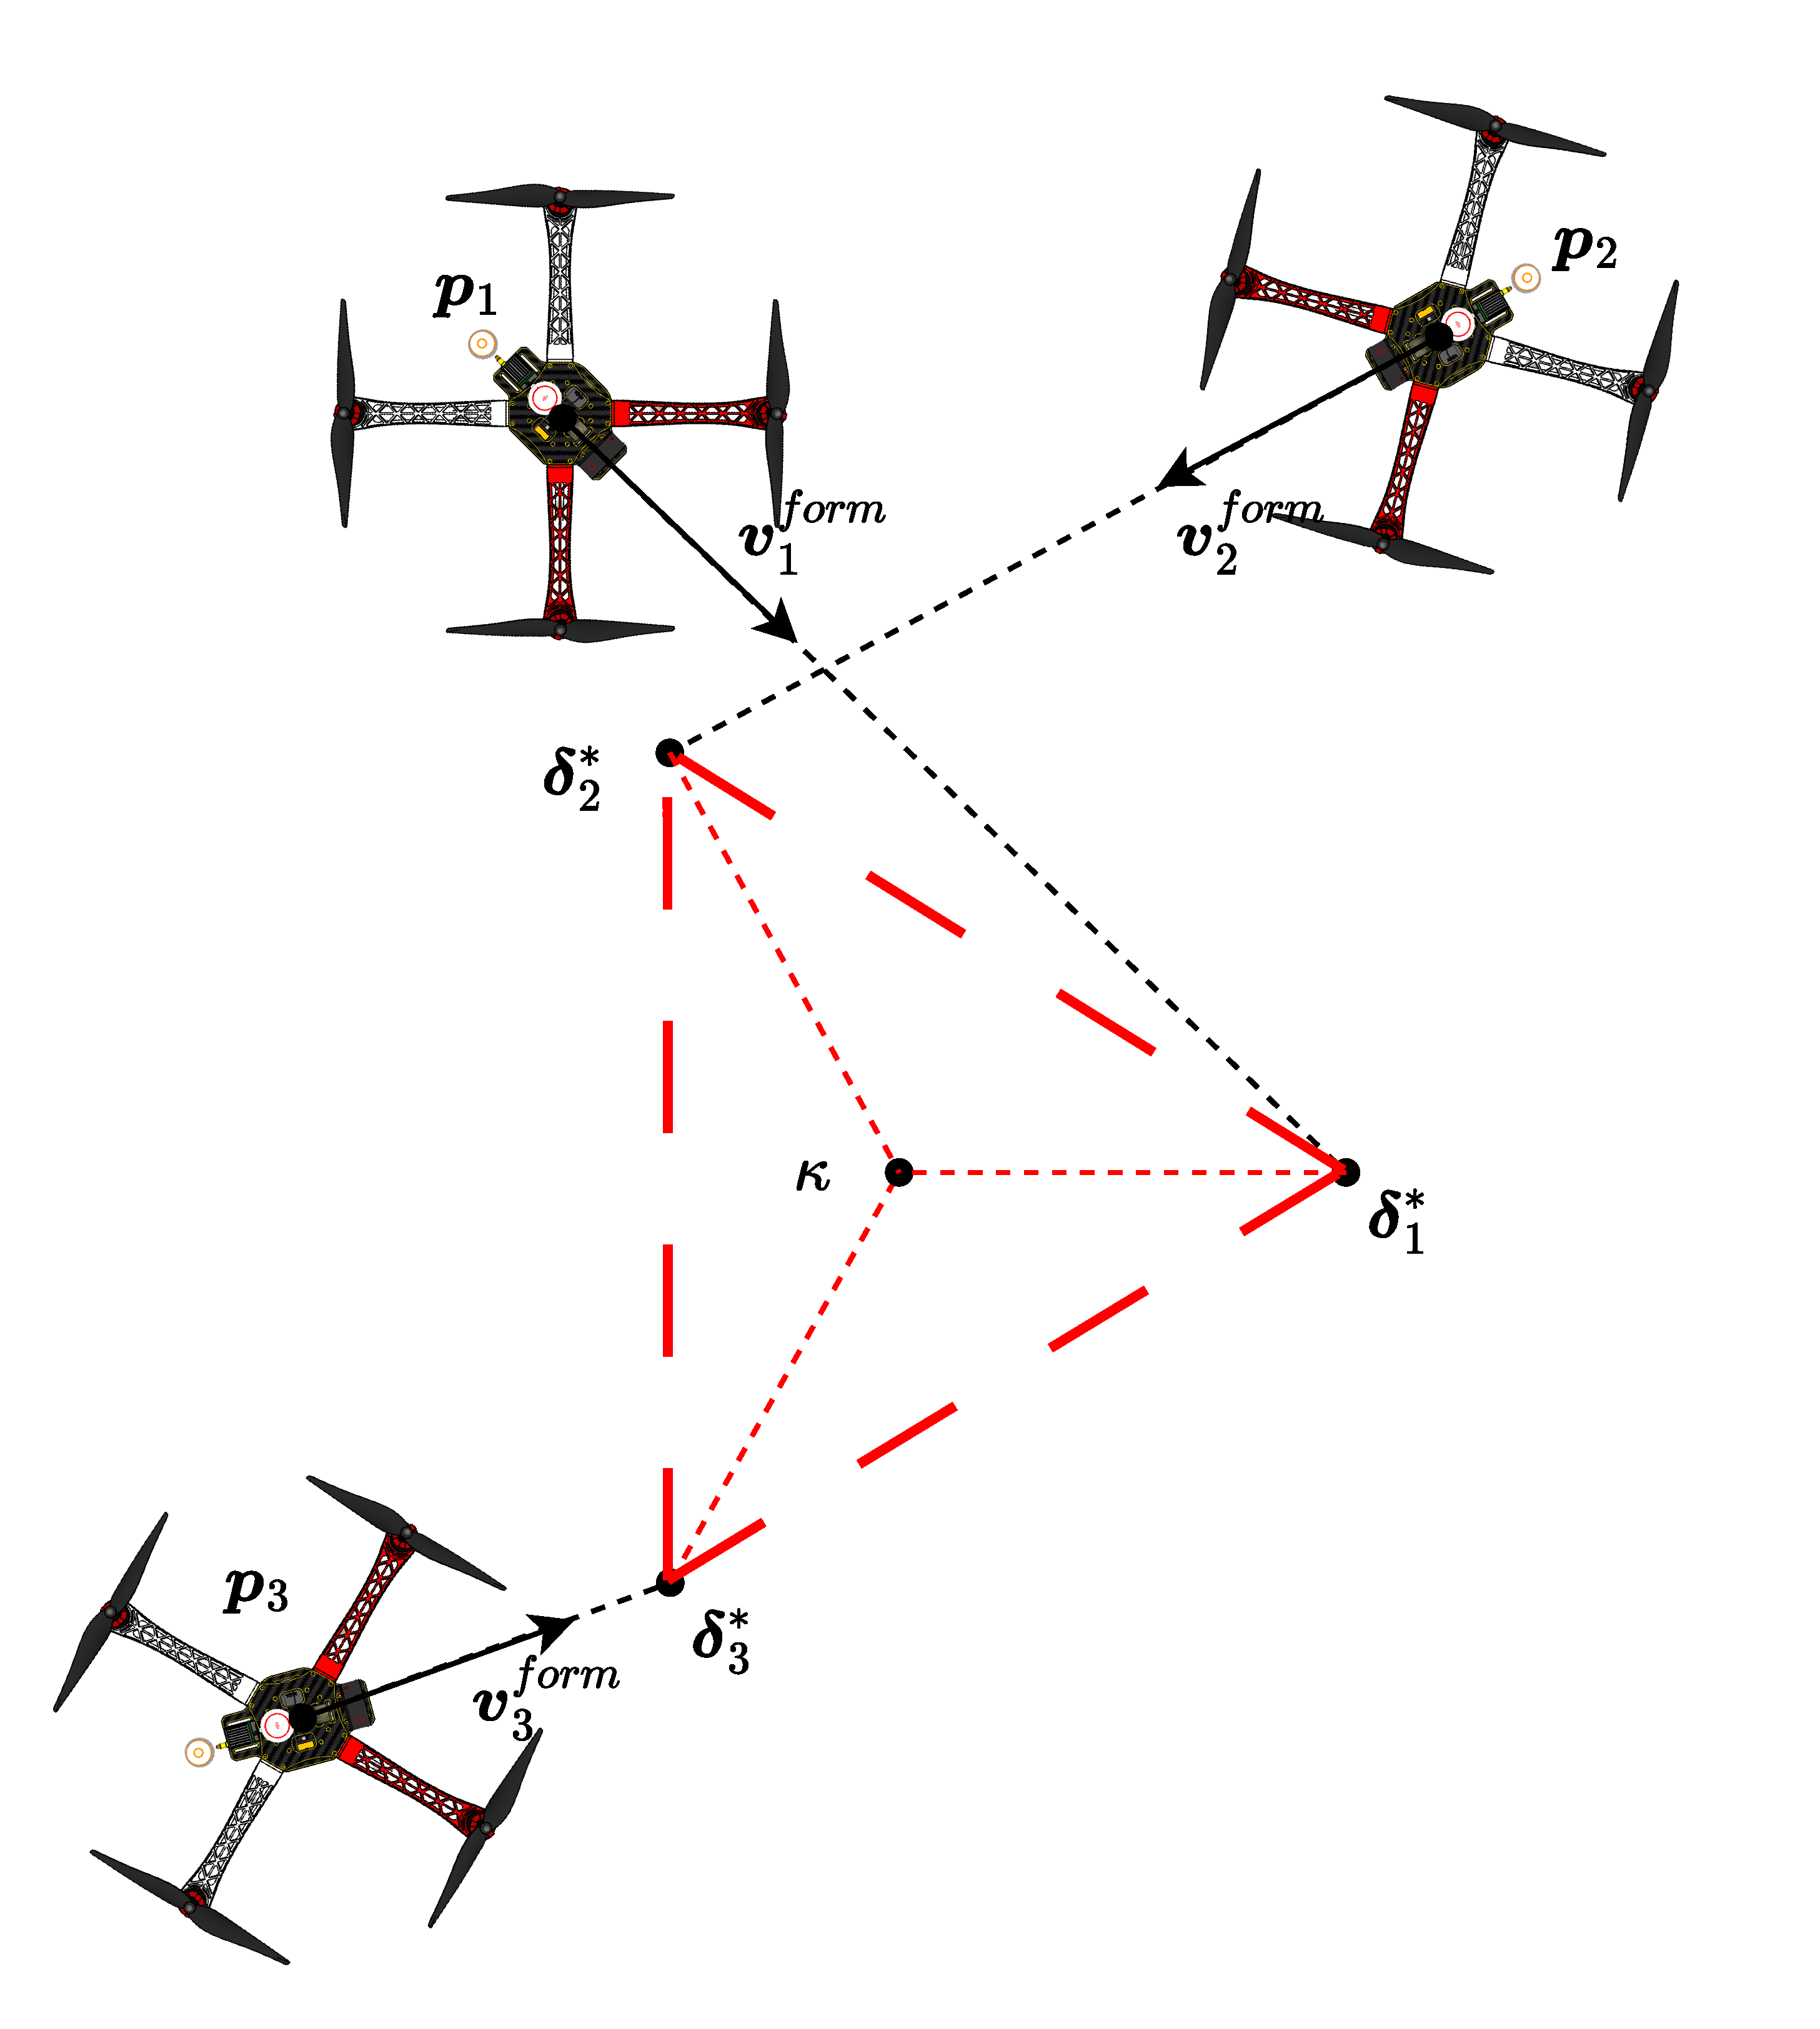
\includegraphics[width=\linewidth]{figures/behavior_formation.pdf} 
                \caption{Formation-Keeping}
                \label{fig:behavior_formation}
            \end{subfigure}
            \hfill
            \begin{subfigure}[b]{0.32\textwidth}
                \centering
                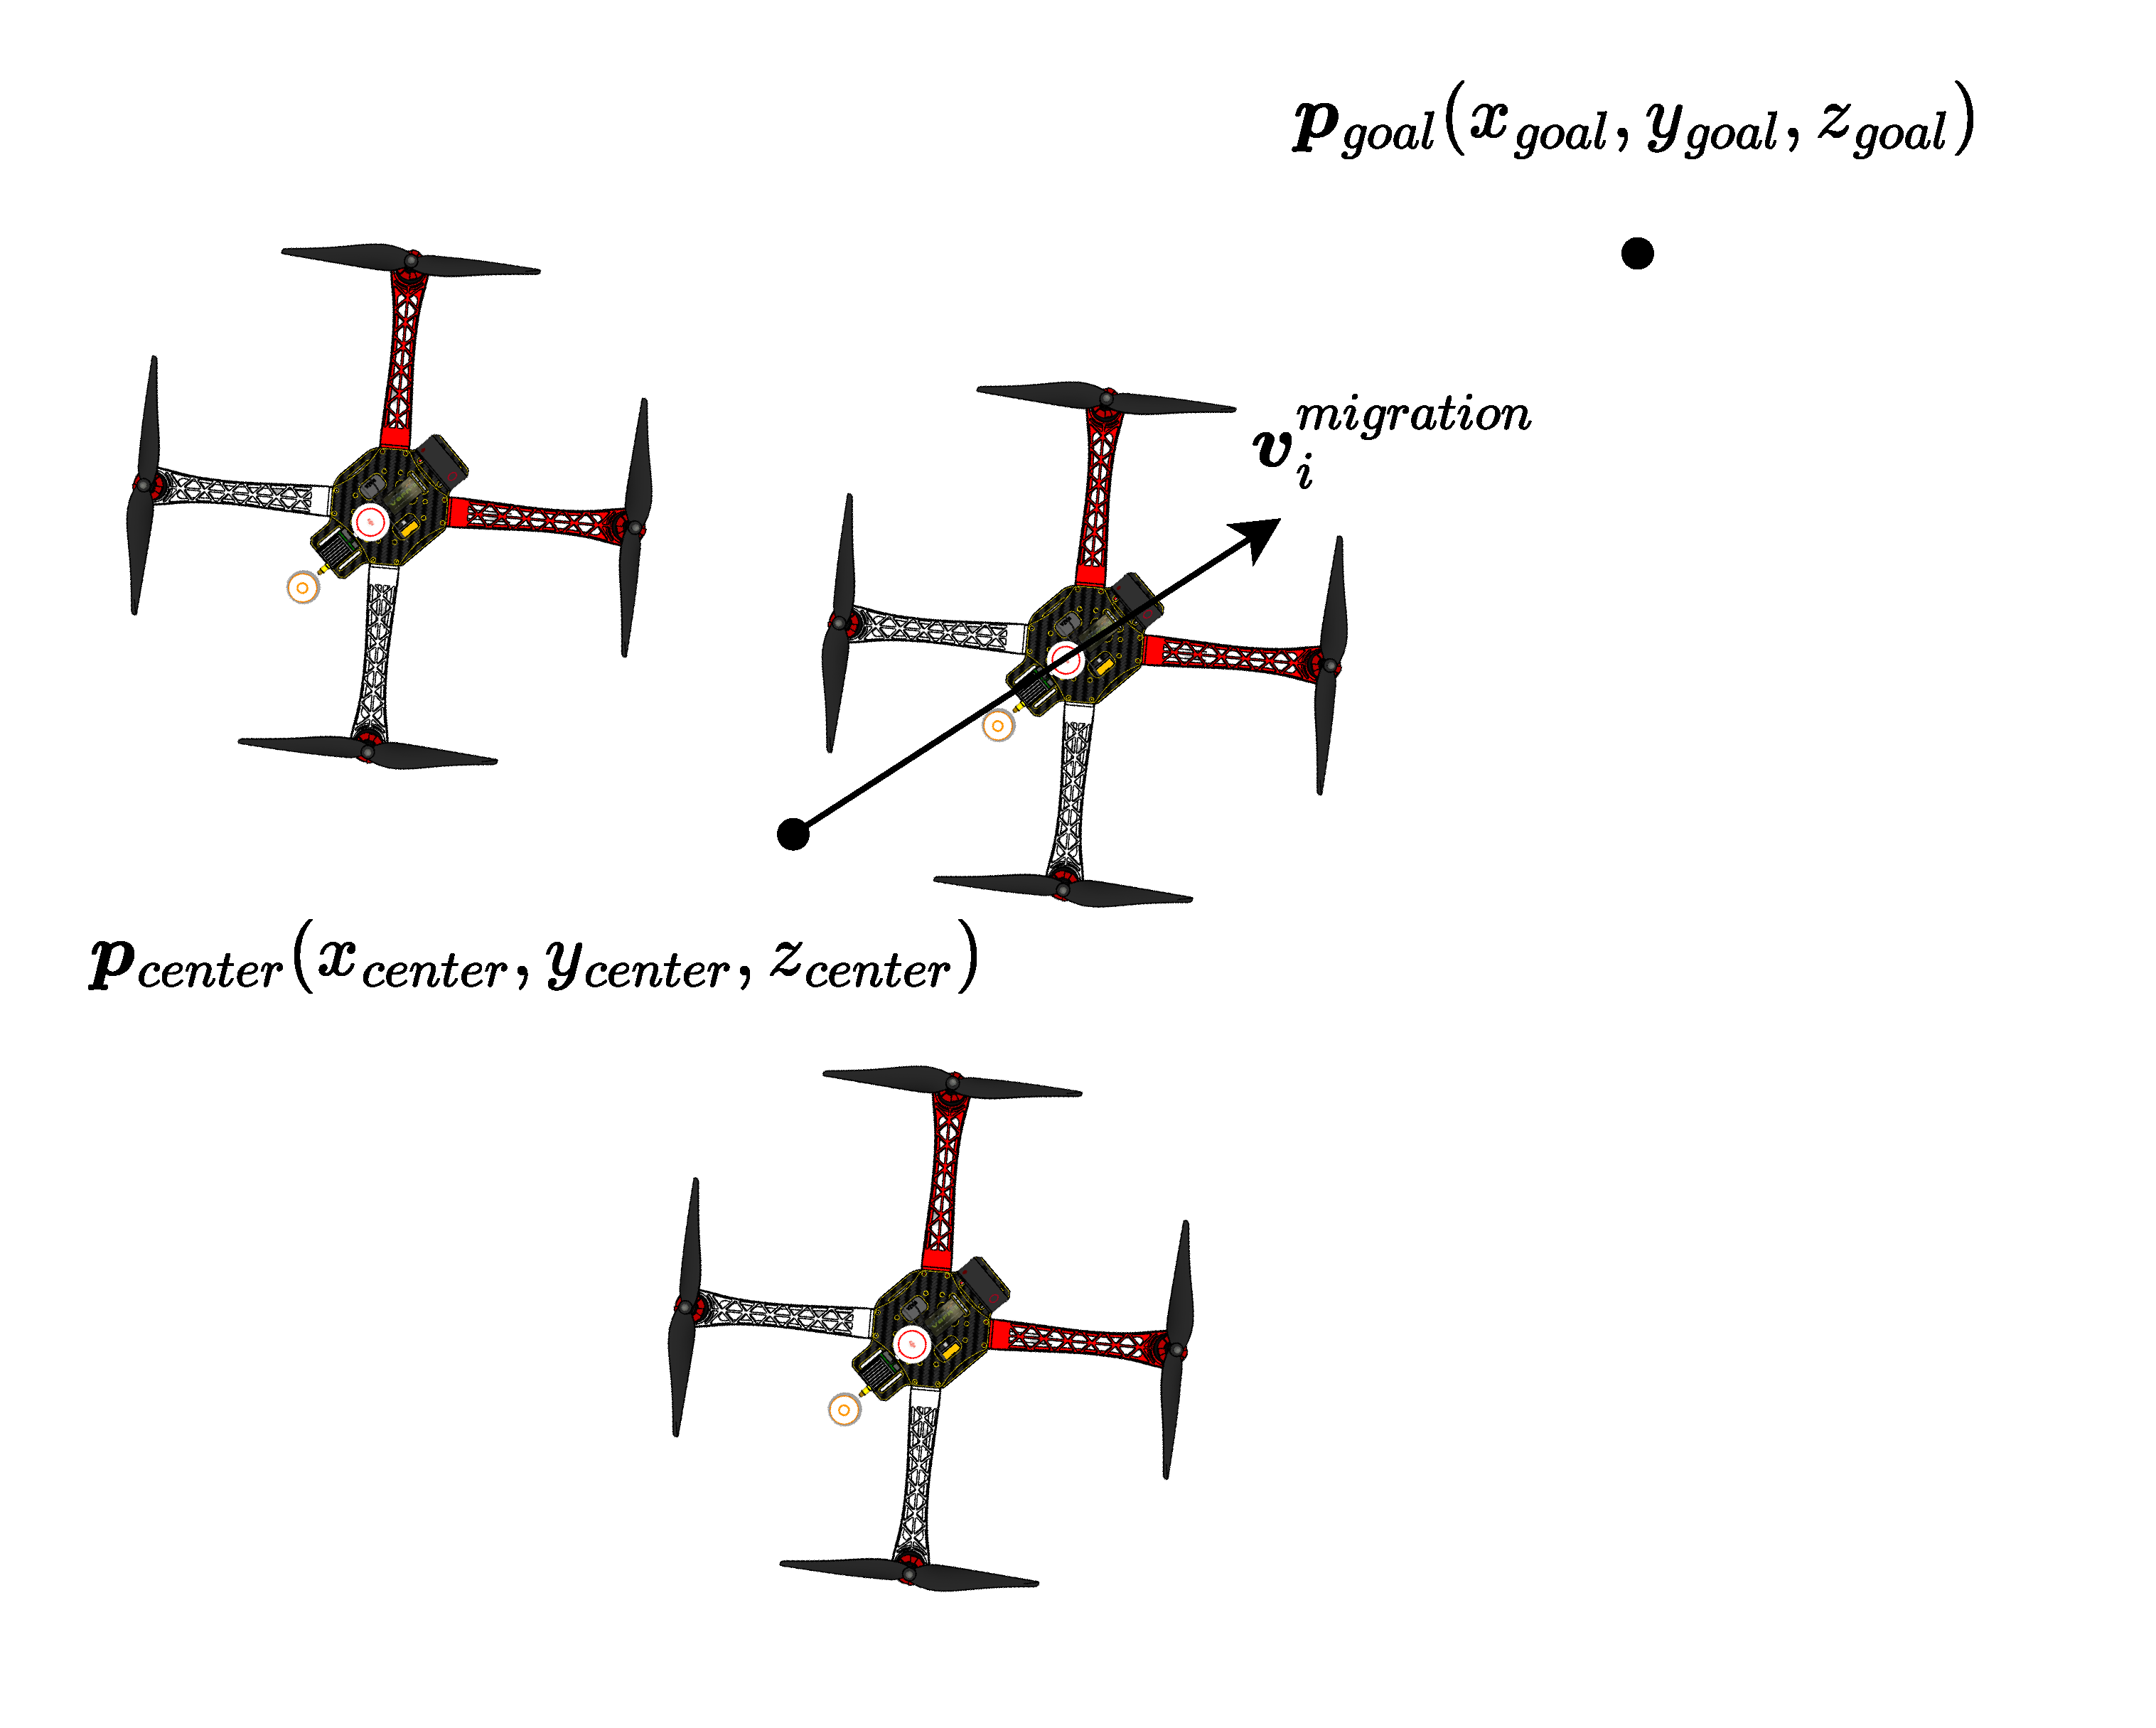
\includegraphics[width=\linewidth]{figures/behavior_migration.pdf} 
                \caption{Migration}
                \label{fig:behavior_migration}
            \end{subfigure}
            \hfill
            \begin{subfigure}[b]{0.32\textwidth}
                \centering
                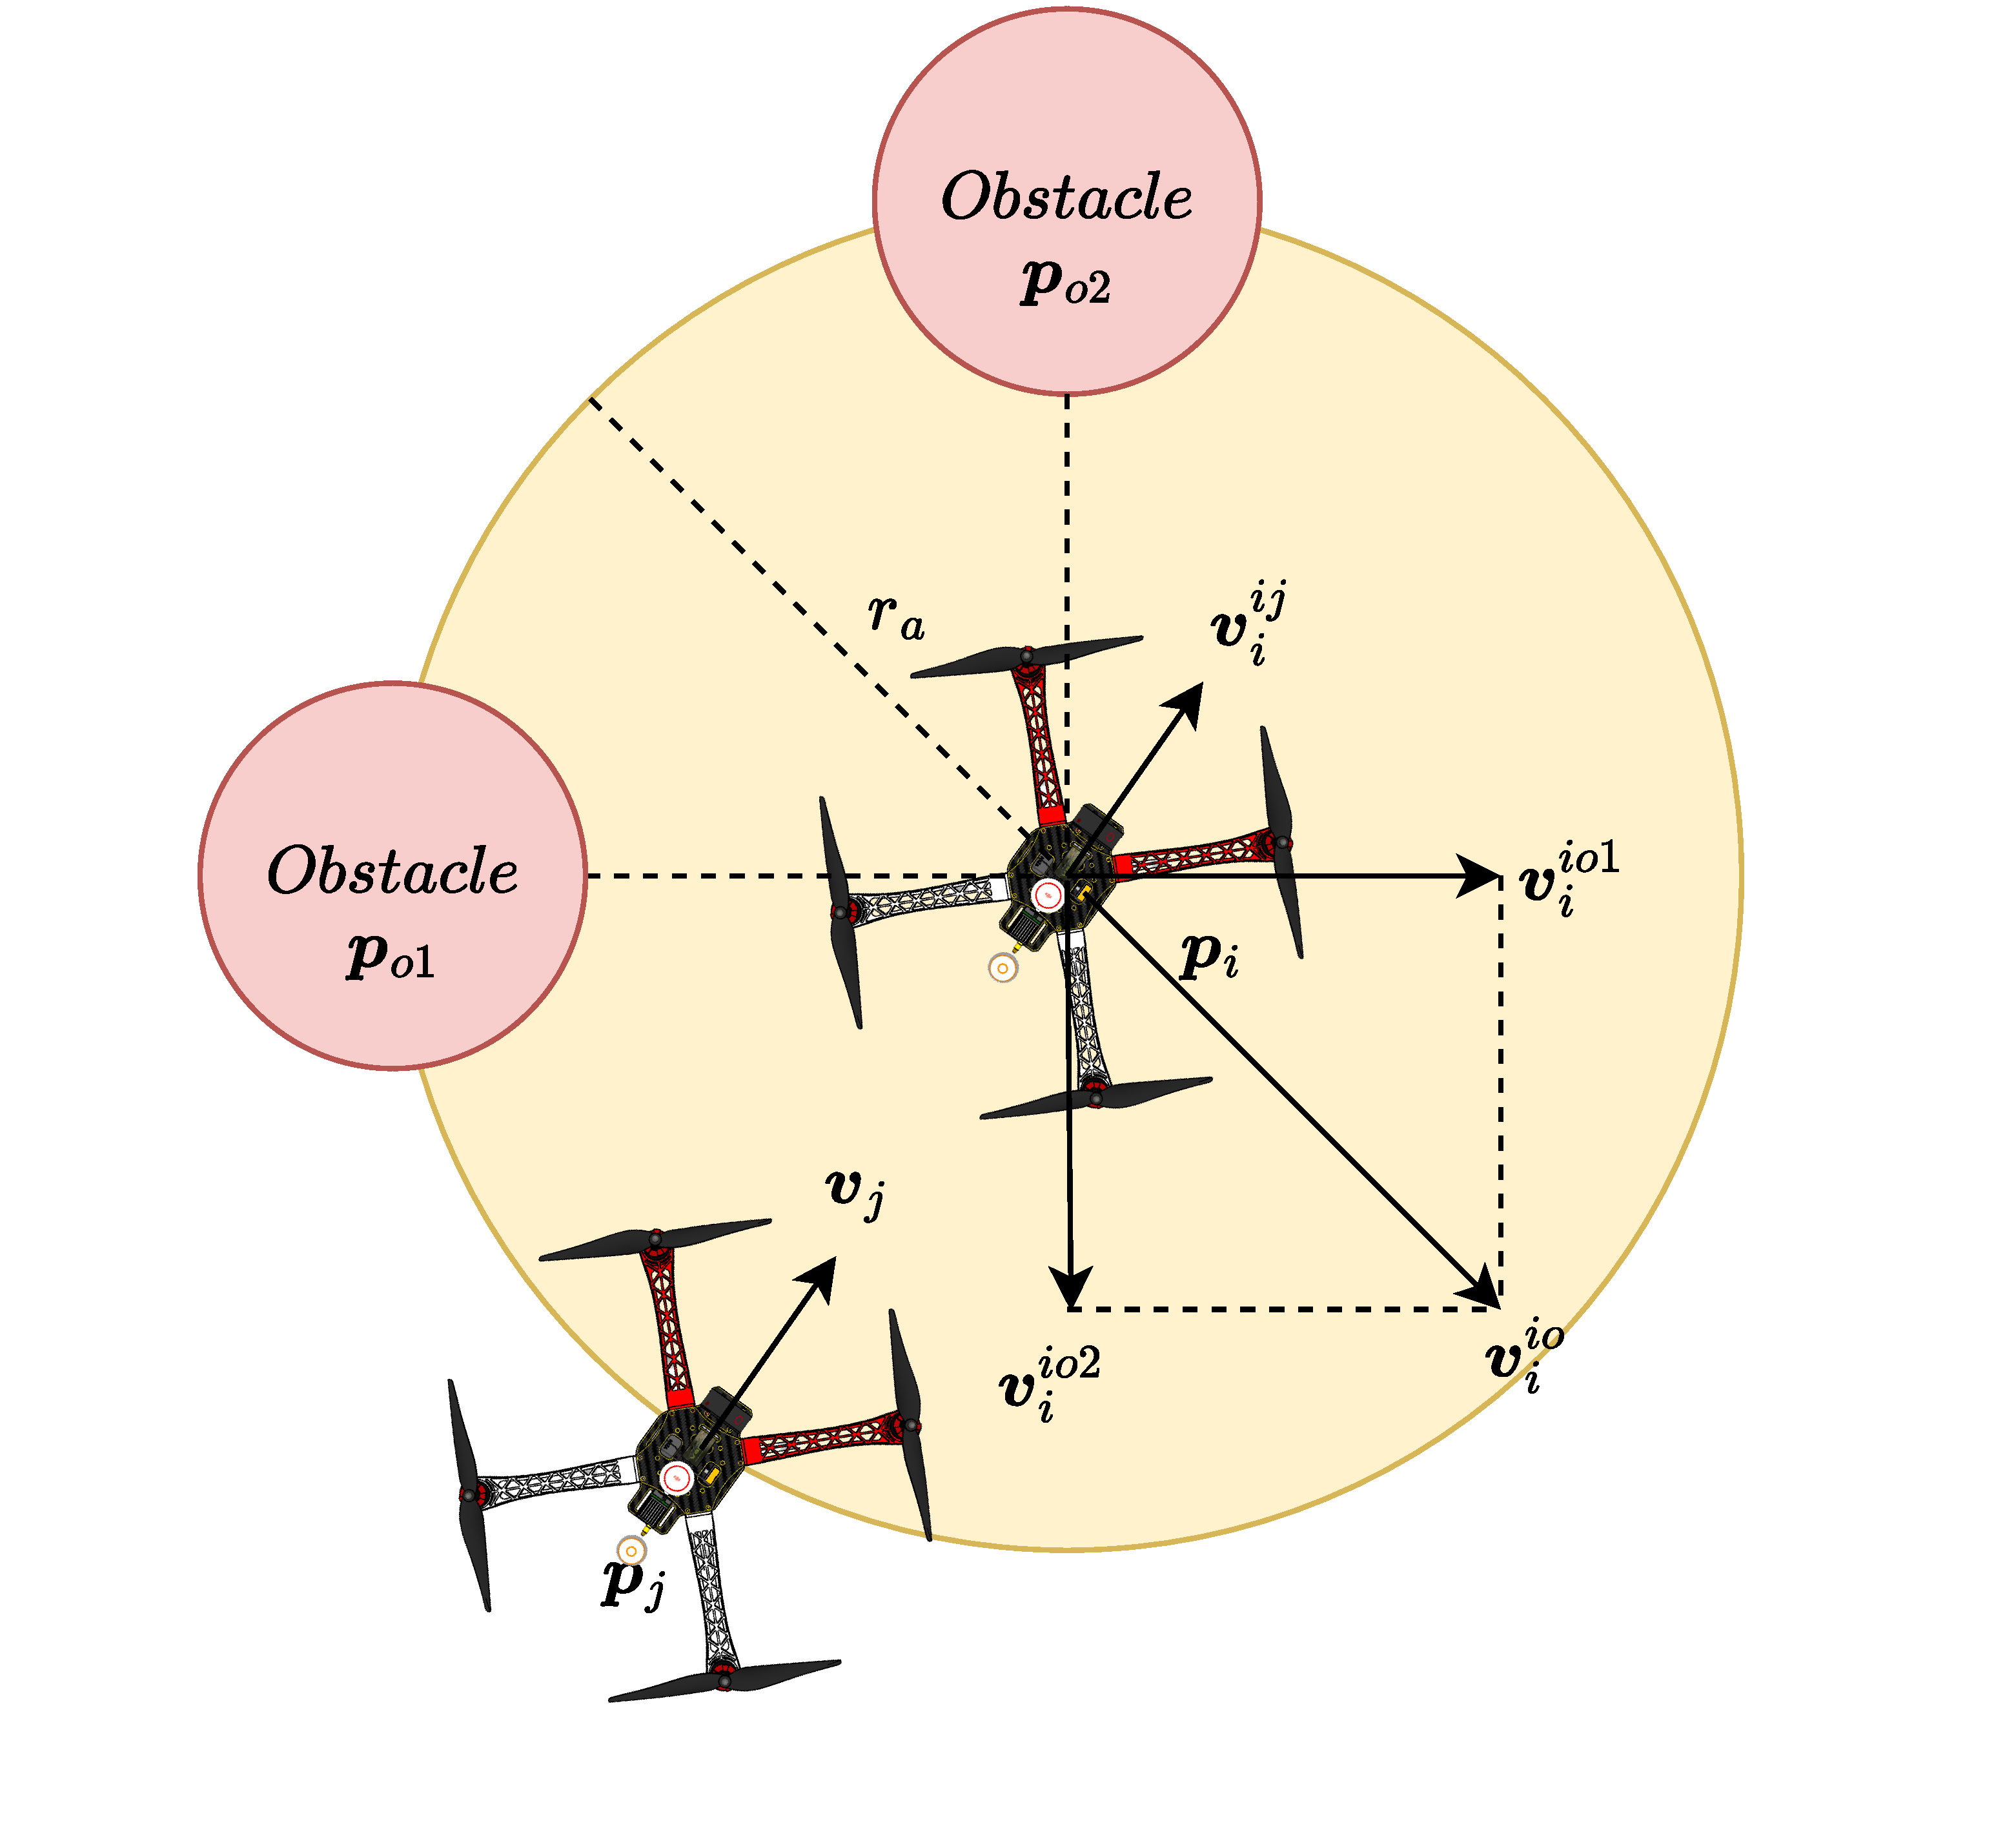
\includegraphics[width=\linewidth]{figures/behavior_avoidance.pdf} 
                \caption{Collision Avoidance}
                \label{fig:behavior_avoidance}
            \end{subfigure}
            \vspace{1em}
            \hfill
            \hfill
            \hfill
            \begin{subfigure}[b]{0.32\textwidth}
                \centering
                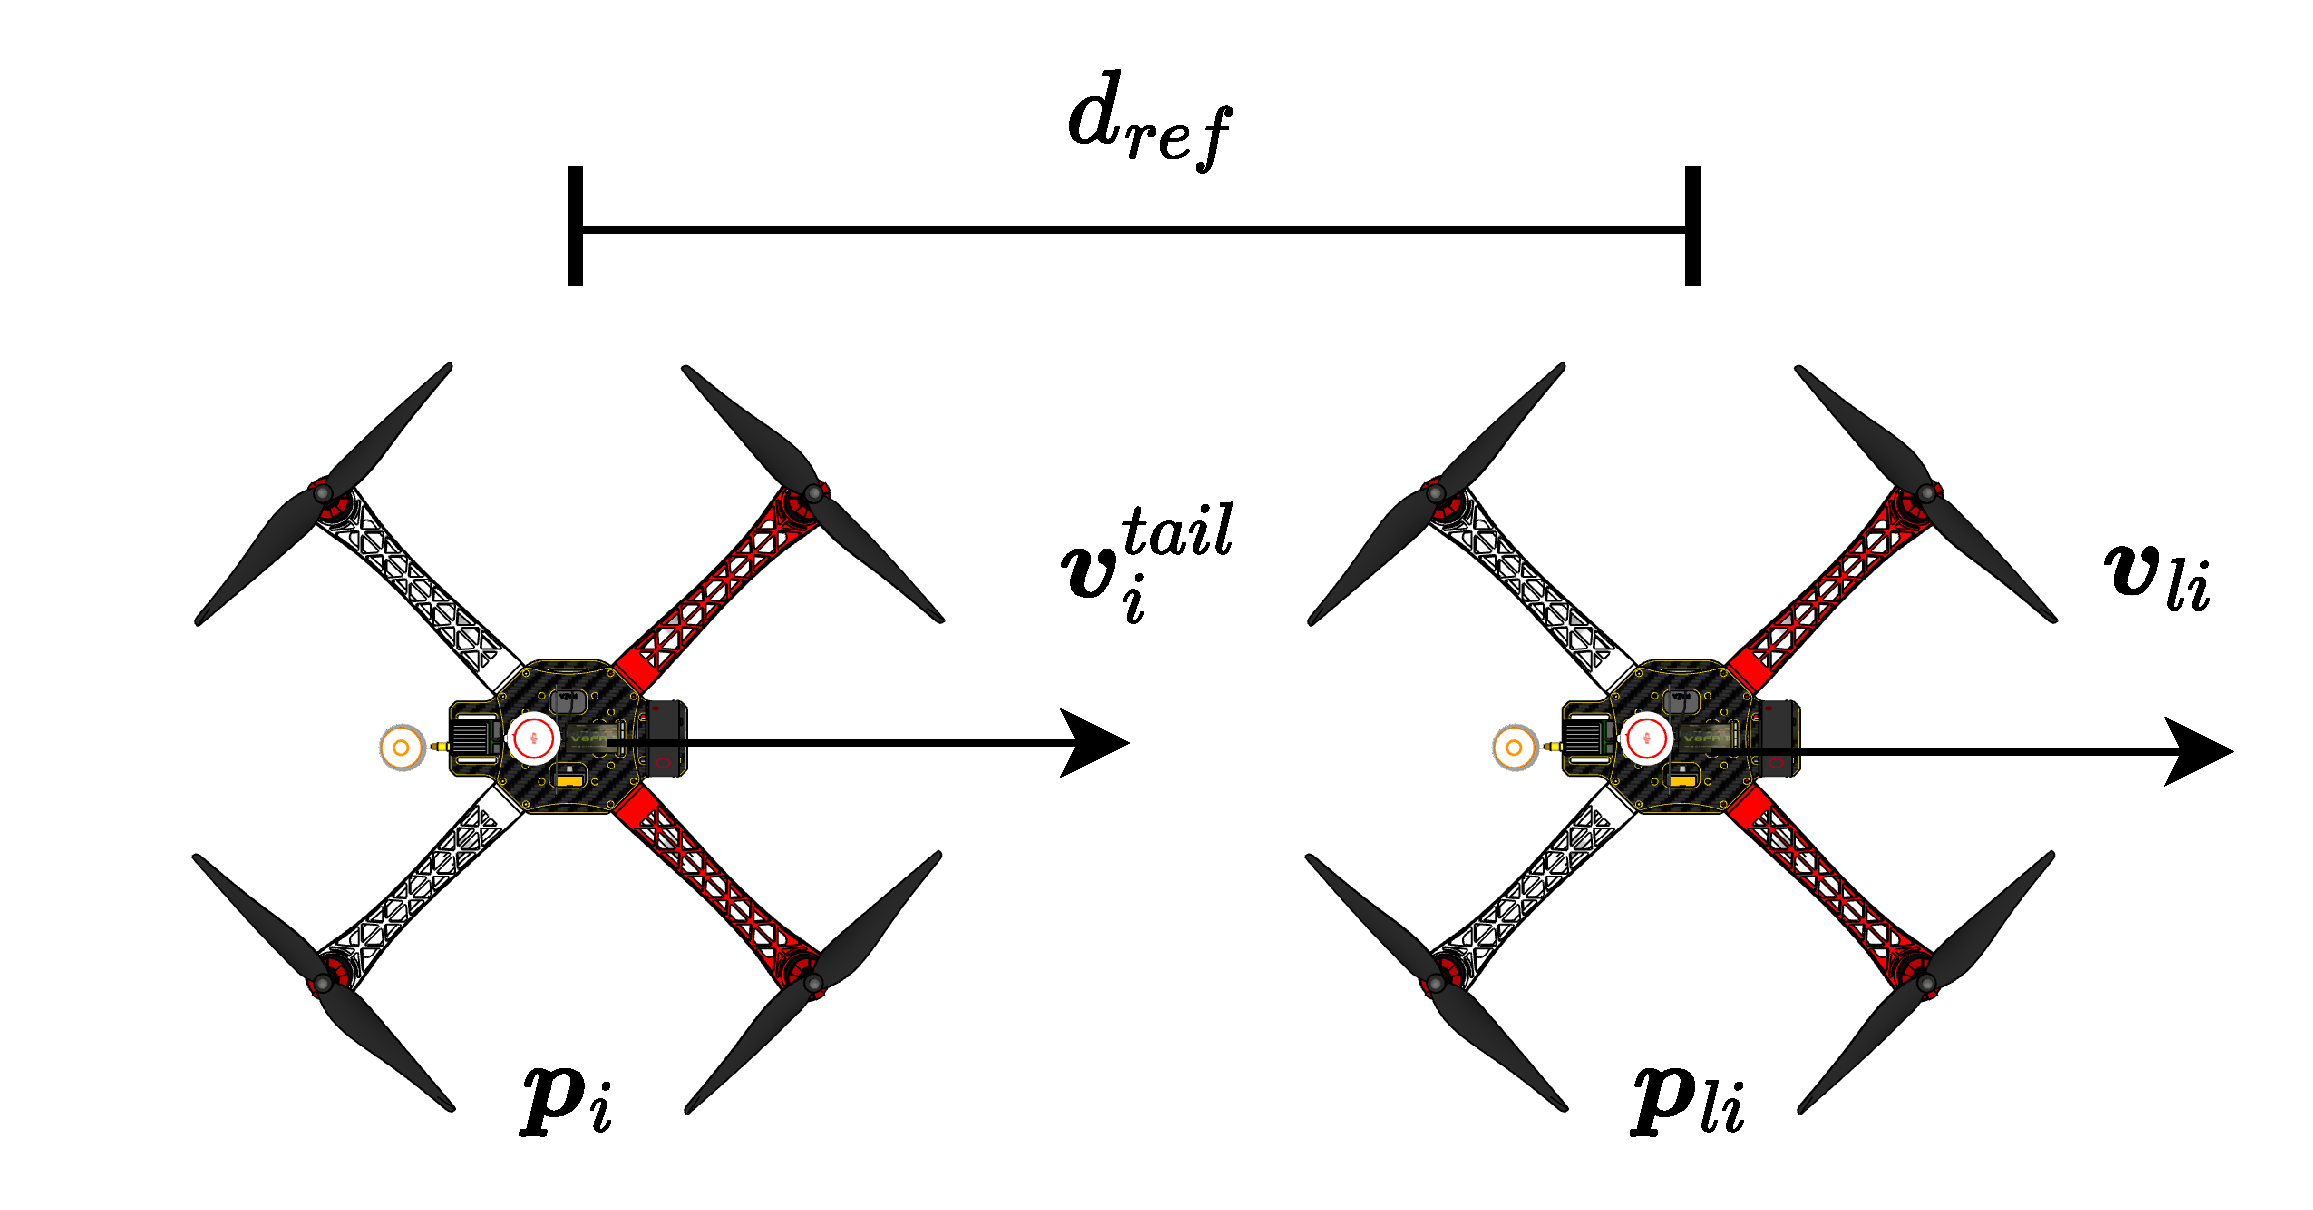
\includegraphics[width=\linewidth]{figures/behavior_tailgating.pdf} 
                \caption{Tailgating}
                \label{fig:behavior_tailgating}
            \end{subfigure}
            \hfill
            \begin{subfigure}[b]{0.32\textwidth}
                \centering
                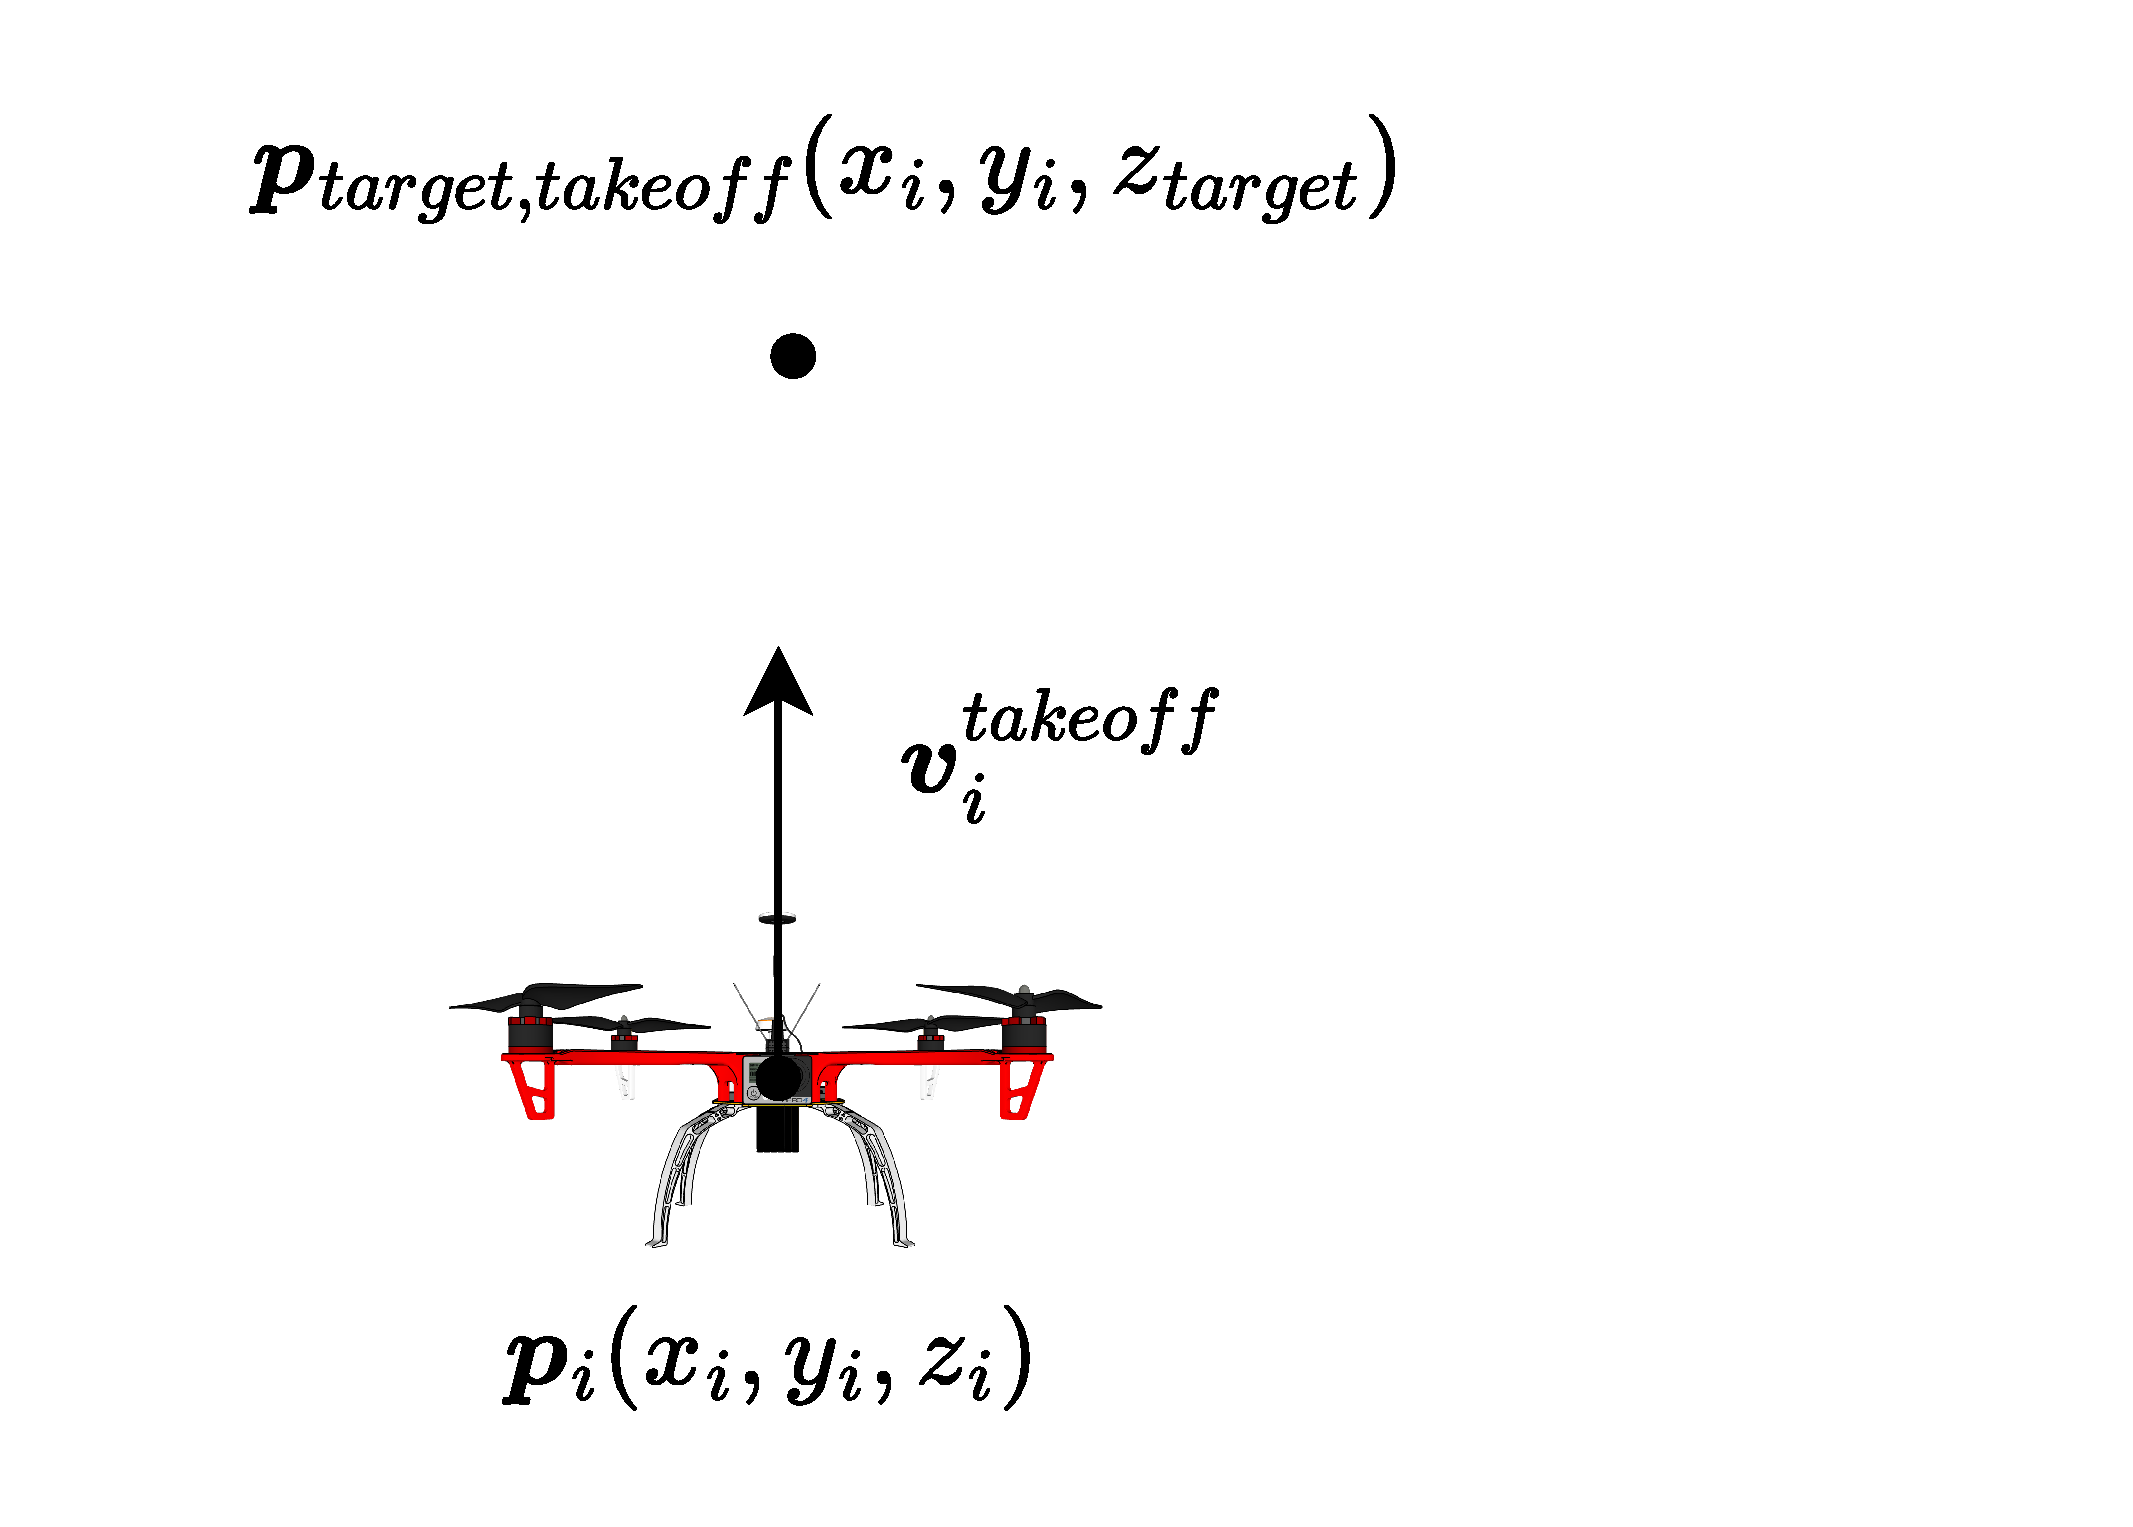
\includegraphics[width=\linewidth]{figures/behavior_takeoff.pdf} 
                \caption{Takeoff}
                \label{fig:behavior_takeoff}
            \end{subfigure}
            \hfill
            \hfill
            \hfill
            
            \caption{Illustration of behavioral components in the high-level planner.}
            \label{fig:behaviors_visual}
        \end{figure}

    \subsection{Behavior Combination Strategies: Static vs. Adaptive}
        Once the takeoff phase is complete and the system enters the mission mode, the planner strategy that governs the interaction between behaviors becomes active. This section details the implementation of the two distinct planner strategies that were comparatively evaluated: the static IAPF and the adaptive ERC. The detailed computational logic for the high-level planner, which encompasses mode transitions, adaptive triggers, and the combination of all behavioral components, is summarized in Algorithm~\ref{alg:high_level_planner}.

        \begin{algorithm}
        \begingroup\small
            \caption{High-Level Planner Pseudocode}
            \label{alg:high_level_planner}
            \begin{algorithmic}[1]
                \State \Comment{Phase 1: Transition Logic from Takeoff}
                \If{swarm.mode == TAKEOFF}
                    \State allReady $\gets$ \textbf{true}
                    \ForAll{agent $i$ in swarm}
                        \If{$|z_{\text{target}} - z_i(t)| > \epsilon_z$}
                            \State allReady $\gets$ \textbf{false}
                            \State \textbf{break}
                        \EndIf
                    \EndFor
                    \If{allReady}
                        \State swarm.mode $\gets$ MISSION
                    \EndIf
                \EndIf

                \State \Comment{Phase 2: Calculate Reference Velocity}
                \ForAll{agent $i$ in swarm}
                    \If{$i.mode == TAKEOFF$} \Comment{Agent is in Takeoff Mode}
                        \State $\boldsymbol{v}_{\text{ref}} \gets \boldsymbol{v}_{i}^{\text{takeoff}} + \boldsymbol{v}_{i}^{\text{ij}} + \boldsymbol{v}_{i}^{\text{io}}$
                    \Else \Comment{Agent is in Mission Mode}
                        \If{STRATEGY == IAPF} \Comment{Static IAPF strategy selected}
                            \State $\boldsymbol{v}_{\text{ref}} \gets \boldsymbol{v}_{i}^{\text{mig}} + \boldsymbol{v}_{i}^{\text{io}} + \boldsymbol{v}_{i}^{\text{ij}} + \boldsymbol{v}_{i}^{\text{form}}$
                        \Else \Comment{Adaptive ERC strategy selected}
                            \State $w_e \gets \text{estimate\_environmental\_width()}$
                            \If{$w_e \le \alpha \cdot r_{\text{agent}}$} \Comment{Tailgating Mode}
                                \State $i.\text{submode} \gets \text{TAILGATING}$
                                \State $\kappa \gets 1.0$
                            \Else
                                \State $i.\text{submode} \gets \text{FORMATION}$ \Comment{Formation Mode}
                                \State $w_f \gets \text{get\_ideal\_formation\_width()}$
                                \If{$w_e - 2r_{\text{agent}} < w_f$} \Comment{Narrowing Step} 
                                    \State $\kappa \gets (w_e - 2r_{\text{agent}}) / w_f$
                                \Else
                                    \State $\kappa \gets 1.0$
                                \EndIf
                            \EndIf
                            \If{$i.\text{submode} == \text{FORMATION}$}
                                \State $\boldsymbol{v}_{\text{ref}} \gets \boldsymbol{v}_{i}^{\text{mig}} + \boldsymbol{v}_{i}^{\text{io}} + \boldsymbol{v}_{i}^{\text{ij}} + \boldsymbol{v}_{i}^{\text{form}}$
                            \Else
                                \State $\boldsymbol{v}_{\text{ref}} \gets \boldsymbol{v}_{i}^{\text{mig}} + \boldsymbol{v}_{i}^{\text{io}} + \boldsymbol{v}_{i}^{ij} + \boldsymbol{v}_{i}^{\text{tail}}$
                            \EndIf
                        \EndIf

                        \State \Comment{Hover Mode (Handle Stagnation)}
                        \If{$\|\boldsymbol{v}_{\text{ref}}\| < \epsilon_v$}
                            \State $\boldsymbol{v}_{\text{ref}} \gets \boldsymbol{0}$
                        \EndIf
                    \EndIf

                    \State \Comment{Phase 3: Update Reference Position}
                    \State $\boldsymbol{p}_{\text{ref}} \gets \boldsymbol{p}_{\text{current}} + \boldsymbol{v}_{\text{ref}} \cdot dt$
                \EndFor
            \end{algorithmic}
        \endgroup
        \end{algorithm}

        \begin{enumerate}
            \item \textbf{Static Strategy (IAPF):} In this non-adaptive approach, all behavioral components are additively combined for robust navigation and formation-keeping. The desired velocity is given by:
            \begin{equation}
                \boldsymbol{v}_{\text{ref}}^{\text{IAPF}}=\boldsymbol{v}_{i}^{\text{mig}}+\boldsymbol{v}_{i}^{io}+\boldsymbol{v}_{i}^{ij}+\boldsymbol{v}_{i}^{\text{form}}
            \end{equation}
            Although effective in open spaces, this "rigid formation" approach has a fundamental limitation: it cannot alter its shape, making it prone to failure when encountering narrow passages where formation integrity conflicts with collision avoidance.
            
            \item \textbf{Adaptive Strategy (ERC):} The ERC strategy is designed to overcome the limitations of IAPF by introducing an adaptive mechanism that alters the swarm's behavior based on environmental conditions. Its governing equation is:
            \begin{equation}
                \boldsymbol{v}_{\text{ref}}^{\text{ERC}}=\boldsymbol{v}_{i}^{\text{mig}}+\boldsymbol{v}_{i}^{io}+\boldsymbol{v}_{i}^{ij}+\sigma_{i}\boldsymbol{v}_{i}^{\text{form}}+(1-\sigma_{i})\boldsymbol{v}_{i}^{\text{tail}}
            \end{equation}
            where $\sigma_i \in \{0, 1\}$ acts as a discrete mode-switching boolean flag.
            
            The core of the ERC strategy is its event-based trigger, which relies on environmental perception to enable adaptive reconfiguration. This process, illustrated in Fig.~\ref{fig:width_estimation}, begins with each agent estimating the available environmental width, $w_e$, in front of it. The agent identifies the nearest obstacle points to its left ($\boldsymbol{o}_l$) and right ($\boldsymbol{o}_r$) relative to its direction of motion, $\boldsymbol{u}_{\text{ref}}$. The environmental width is then calculated as the projection of the vector connecting these two points onto the axis perpendicular to the direction of motion, $\boldsymbol{u}_{\text{ref}}^{\perp}$, as given by:
            \begin{equation}
                w_{e}=|\langle(\boldsymbol{o}_{r}-\boldsymbol{o}_{l}), \boldsymbol{u}_{\text{ref}}^{\perp}\rangle|
                \label{eq:width_estimation}
            \end{equation}
            where $\langle\cdot,\cdot\rangle$ denotes the dot product.

            \begin{figure}
                \centering
                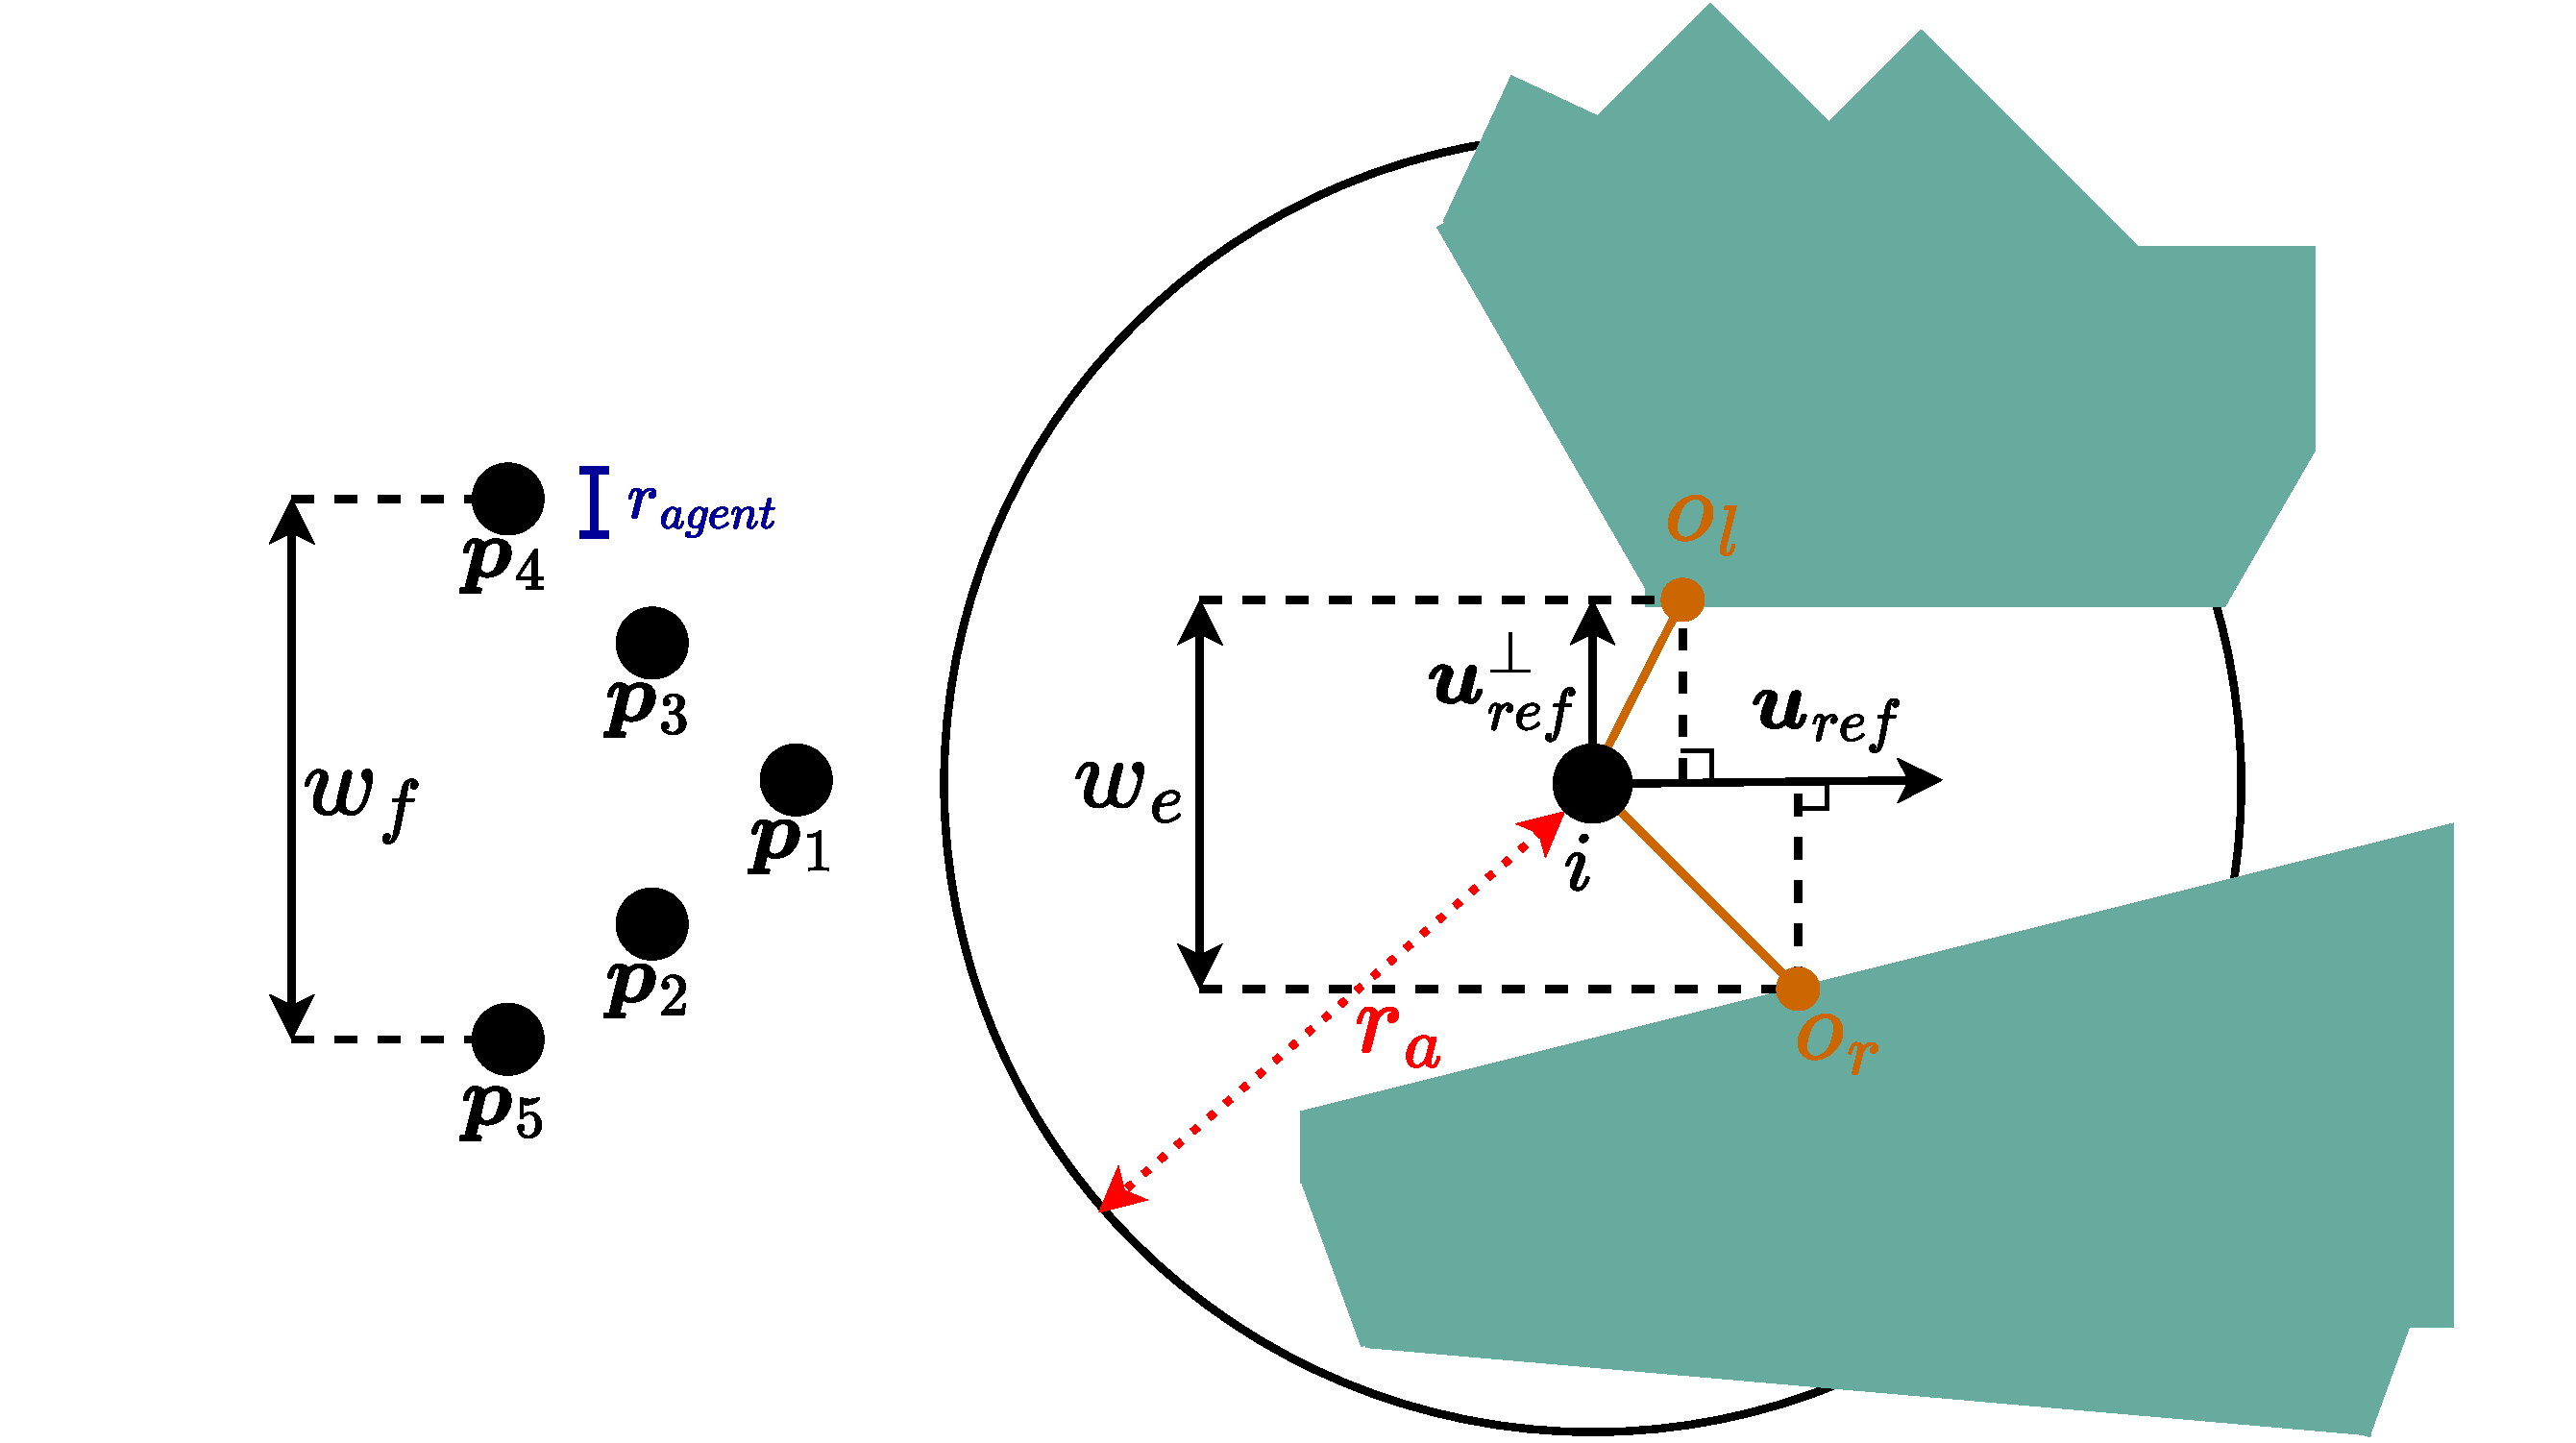
\includegraphics[width=0.75\columnwidth]{figures/width_estimation.pdf}
                \caption{Mechanism for estimating the environmental width ($w_e$) based on the nearest obstacle points ($o_l$, $o_r$) relative to the agent's direction of motion ($u_{\text{ref}}$).}
                \label{fig:width_estimation}
            \end{figure}

            This estimated width enables a two-tiered adaptive response. First, if $w_e$ is smaller than the ideal formation width ($w_f$), the system attempts to compress the formation by adjusting the scaling factor, $\kappa$. Second, if the space becomes critically narrow, a full mode switch is triggered, causing $\sigma_i$ to transition from 1 to 0.
            
            \begin{itemize}
                \item \textbf{Formation Scaling:} If $w_e$ is smaller than the ideal formation width ($w_f$) but still permits multi-agent traversal, the planner adjusts the scaling factor ($\kappa \le 1.0$) to compress the topology laterally:
                \begin{equation}
                    \kappa=\frac{w_{e}-2r_{\text{agent}}}{w_{f}}
                \end{equation}
                where $r_{\text{agent}}$ represents the physical radius of the quadcopter.
                
                \item \textbf{Mode Switching to Tailgating:} If the environmental width ($w_e$) becomes very narrow, a full mode switch is triggered. The condition for this transition is:
                \begin{equation}
                    w_{e} \le \alpha \cdot r_{\text{agent}}
                \end{equation}
                where $\alpha$ is a tunable clearance factor. Upon triggering, $\sigma_i$ evaluates to $0$, overriding the formation structure and activating single-file tailgating. Each agent identifies its local leader ($l_i$) as the closest agent directly ahead on the migration axis ($\boldsymbol{u}_{\text{ref}}$):
                \begin{equation}
                    l_i = \begin{cases} \arg\min_{j:\tilde{p}_{ij}>0} \tilde{p}_{ij}, & \text{if } \{j \mid \tilde{p}_{ij} \ge 0\} \neq \emptyset \\ -1, & \text{otherwise} \end{cases}
                \end{equation}
                where $\tilde{p}_{ij} = \langle(\boldsymbol{p}_{j}-\boldsymbol{p}_{i}), \boldsymbol{u}_{\text{ref}}\rangle$. An index of $-1$ delegates the agent as the current swarm leader. 
                
                This specific criterion---selecting the local leader based strictly on the maximum forward projection---was deliberately chosen over topology-based alternatives (e.g., selecting a central agent) or environment-based alternatives (e.g., maximum distance from obstacles). Designating a central agent would kinematically force the leading half of the swarm to maneuver backward to fall in line, drastically increasing collision risks and reorganization delays. Furthermore, obstacle-proximity criteria are highly susceptible to localized sensor noise and irregular wall geometries, which can induce unstable, high-frequency leader switching (chattering). In contrast, the forward-projection method naturally and instantly sorts the agents into a sequential queue based on their existing spatial distribution, minimizing crossing paths. Crucially, this assignment is fully decentralized; if a front-most agent is removed or fails, the subsequent agent automatically re-indexes its local leader to $-1$ and assumes the lead role, ensuring robust chain navigation without requiring global reassignment.
            \end{itemize}

            Finally, to mitigate minor local minima blockages, a localized stagnation check is enforced. If the aggregated reference magnitude falls below a minimal threshold ($||\boldsymbol{v}_{\text{ref}}|| < \epsilon_v$), the vector is clamped to zero ($\boldsymbol{0}$), ensuring a stable hover rather than generating erratic micro-oscillations.
        \end{enumerate}

\section{Simulation Setup and Performance Metrics}
    To validate the proposed control system and comparatively evaluate the IAPF and ERC strategies, a comprehensive simulation framework was developed. This section details the simulation environment, the physical and control parameters used, the design of the experimental scenarios, and the metrics for quantitative performance analysis.

    \subsection{Simulation Environment and System Parameters}
        The entire system was implemented and tested in a custom simulator developed in Python, utilizing an Object-Oriented Programming (OOP) paradigm. The simulation models a swarm of five homogeneous quadcopters, with the physical parameters of each agent based on the DJI F450 frame. The key physical parameters and operational constraints are provided in Appendix~\ref{sec:app_parameters} (Table~\ref{tab:physical_params}). The nonlinear equations of motion were solved numerically at each timestep using the Dormand-Prince 5(4) adaptive step size integrator, with absolute and relative tolerances set to $10^{-6}$ to ensure high-fidelity results.

        The control parameters for both low-level and high-level controllers were predefined and are provided in Appendix~\ref{sec:app_parameters} (Tables~\ref{tab:low_level_params} and \ref{tab:high_level_params}). The static gains for the cascaded PID low-level controller were adopted from the work of John Bass \citep{john_bobzwikquadcopter_simcon_2025}, as it uses an identical physical and dynamic model, ensuring a stable and reliable foundation for each agent. For the high-level planner, the parameters were heuristically tuned with a primary reference to Bui et al. \citep{bui_event-based_2025}, prioritizing safety (higher avoidance gains) over formation rigidity.

        Furthermore, it should be explicitly noted that the simulated environment exclusively features static obstacles. The primary focus of this study is to evaluate the spatial reconfiguration capabilities of the ERC planner in constrained spaces and its robustness to aerodynamic disturbances. The integration of dynamic or moving obstacles would require additional predictive avoidance logic at the swarm-planner level, which falls outside the scope of the current work. Similarly, the simulation assumes ideal state estimation and instantaneous inter-agent communication. Isolating the system from stochastic sensor noise (e.g., GPS drift) and network latency ensures that the evaluation purely reflects the algorithmic efficacy of the topological reconfiguration logic.

    \subsection{Test Scenarios} \label{sec:test_scenarios}
        To evaluate the system's performance, adaptability, and robustness, six simulation scenarios were designed in a 3D environment, as illustrated in Fig.~\ref{fig:sim_env_3d}. The scenario geometry (obstacles, goals, and waypoints) is defined in the NED inertial frame; however, since the missions are executed at a regulated operating altitude, the trajectory results are reported using the horizontal $x$--$y$ projection. All scenarios use the same autonomous takeoff and formation establishment procedure, with the five agents starting from the following initial positions (in meters): $\boldsymbol{p}_1=[-3,4,0]$, $\boldsymbol{p}_2=[-5,5,0]$, $\boldsymbol{p}_3=[-2,4,0]$, $\boldsymbol{p}_4=[-5,-2,0]$, and $\boldsymbol{p}_5=[-2,-2,0]$.

        \begin{figure}
            \centering
            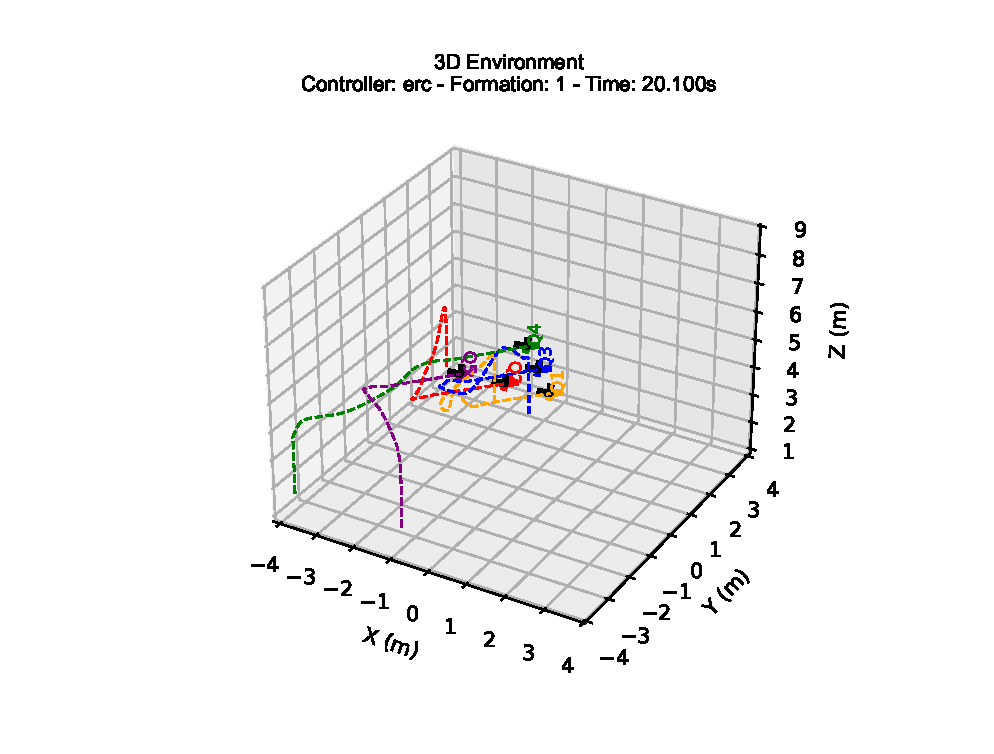
\includegraphics[width=0.9\linewidth]{figures/sim_env_3d.eps}
            \caption{3D simulation environment.}
            \label{fig:sim_env_3d}
        \end{figure}

        \begin{enumerate}
            \item \textbf{Scenario 1 --- Basic Obstacle Avoidance:} The swarm navigates through scattered static obstacles toward a common final goal at $\boldsymbol{p}_{\text{goal}}=[22,3,5]$. This scenario serves as a baseline feasibility test for nominal obstacle avoidance and formation maintenance, and it provides a direct comparison between the IAPF and ERC planners under non-constrained conditions.
            
            \item \textbf{Scenario 2 --- Narrow Gap Passage:} The swarm is tasked with reaching the same final goal $\boldsymbol{p}_{\text{goal}}=[22,3,5]$ while traversing a passage that is narrower than the nominal formation width. This scenario provides a direct comparison between the rigid IAPF strategy (expected to fail) and the adaptive ERC strategy (expected to succeed via formation scaling and tailgating reconfiguration).

            \item \textbf{Scenario 3 --- Wind Disturbance:} This scenario repeats Scenario 2 while applying an external aerodynamic disturbance to evaluate the system's robustness. As illustrated in Fig.~\ref{fig:wind_model}, a periodic and pulsative wind gust is applied globally across the environment during the narrow-gap maneuver. The wind model has a median base velocity of 2.0 m/s and blows from a specific direction characterized by a horizontal yaw angle of $q_{w1} = 180^\circ$ and a vertical pitch angle of $q_{w2} = -5^\circ$. The gust profile operates on a 10-second cycle, featuring a 4-second active burst where the velocity fluctuates with an amplitude of 2.0 m/s at a frequency of 0.25 Hz. This results in peak wind speeds up to 4.0 m/s, severely testing the swarm's stability.
            
            \item \textbf{Scenario 4 --- Topological Trap:} The swarm navigates toward $\boldsymbol{p}_{\text{goal}}=[22,3,5]$ in a concave "U-Trap" environment to reveal limitations of the purely reactive planner in the presence of local minima.
            
            \item \textbf{Scenario 5 --- Waypoint Navigation:} The swarm is tasked with following a multi-segment trajectory defined by a sequence of five precise 3D waypoints: $\boldsymbol{w}_1=[0,5,-5]$, $\boldsymbol{w}_2=[0,0,-5]$, $\boldsymbol{w}_3=[3,-5,-5]$, $\boldsymbol{w}_4=[0,-6,-5]$, and $\boldsymbol{w}_5=[0,0,-5]$. To validate the multi-goal navigation extension and formation orientation mechanism during sharp direction changes, three static rectangular obstacles are placed along the route. The obstacle boundaries are specified by their horizontal $(x,y)$ footprint and vertical $(z)$ altitude span: Obstacle 1 at $(x\in[0.0, 0.2], y\in[2.5, 3.0])$ with $z\in[-1, 7]$ m; Obstacle 2 at $(x\in[-2.5, -1.5], y\in[2.5, 3.0])$ with $z\in[-1, 6]$ m; and Obstacle 3 at $(x\in[2.0, 2.5], y\in[-2.0, -1.5])$ with $z\in[0, 5]$ m.
            
            \item \textbf{Scenario 6 --- Circular Path Tracking:} The swarm is tasked with tracking a continuous circular trajectory with a radius of $r=4$ m while simultaneously avoiding static obstacles. Similar to the previous scenario, the environment contains three localized obstacles positioned at $(x\in[0.0, 0.2], y\in[2.5, 3.0])$ with $z\in[-1, 7]$ m, $(x\in[-2.0, -1.5], y\in[2.5, 3.0])$ with $z\in[-1, 6]$ m, and $(x\in[2.0, 2.5], y\in[-2.0, -1.5])$ with $z\in[0, 5]$ m. This scenario validates the system's ability to maintain continuous trajectory tracking along with a cohesive and dynamically oriented formation.
        \end{enumerate}

        \begin{figure}
            \centering
            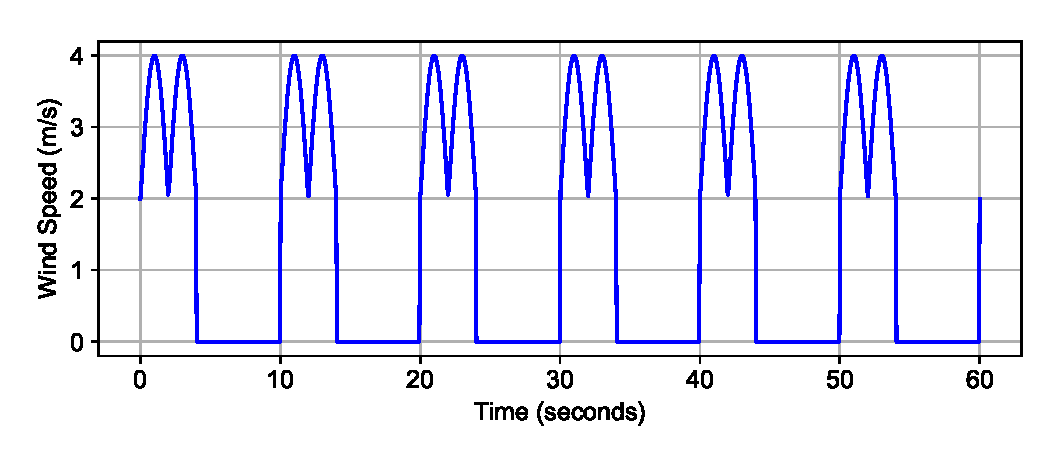
\includegraphics[width=\linewidth]{figures/wind_gust.eps}
            \caption{The periodic wind gust model used for robustness testing.}
            \label{fig:wind_model}
        \end{figure}

    \subsection{Performance Metrics}
        To objectively evaluate the swarm's performance, two primary categories of quantitative metrics were defined. These metrics are designed to measure two fundamental aspects of the mission: the operational accuracy in executing mode-specific tasks and cohesiveness of the collective movement.

        \subsubsection{Operational Accuracy: Mode-Dependent RMSE}
            Since each phase of the mission has a different objective, the error metric is adapted to the currently active mode. This ensures that the system's performance is measured against a relevant goal at any given time. Three specific Root Mean Squared Error (RMSE) metrics are defined as follows:

            \begin{itemize}
                \item \textbf{Takeoff Altitude RMSE ($RMSE_{\text{takeoff}}$):} Active during the takeoff mode, this metric measures the average vertical deviation of all agents from the target altitude, $z_{\text{target}}$. It is used to evaluate the efficiency and uniformity of the ascent process.
                \begin{equation}
                    RMSE_{\text{takeoff}}(t)=\sqrt{\frac{1}{N}\sum_{i=1}^{N}(z_{i}(t)-z_{\text{target}})^{2}}
                \end{equation}

                \item \textbf{Formation Accuracy RMSE ($RMSE_{\text{formation}}$):} Active during the formation mode, this is the primary metric for geometric accuracy. Calculate the average deviation of the distance between all unique pairs of agents from their ideal distance as defined by the formation topology.
                \begin{equation}
                    RMSE_{\text{formation}}(t)=\sqrt{\frac{1}{M}\sum_{\text{pairs}}(||\boldsymbol{p}_{ij}(t)||-||\boldsymbol{\delta}_{ij}^{*}||)^{2}}
                \end{equation}
                where $M$ is the total number of unique pairs in the swarm.

                \item \textbf{Tailgating Distance RMSE ($RMSE_{\text{tailgating}}$):} Active during tailgating mode, this metric measures how well follower agents maintain the specified safe distance, $d_{\text{ref}}$, from their designated leaders.
                \begin{equation}
                    RMSE_{\text{tailgating}}(t)=\sqrt{\frac{1}{N_{f}}\sum_{i\in \text{followers}}(||\boldsymbol{p}_{i}(t)-\boldsymbol{p}_{li}(t)||-d_{\text{ref}})^{2}}
                \end{equation}
                where $N_f$ is the number of follower agents.
            \end{itemize}

            To provide a single scalar value representing the overall operational accuracy for an entire mission, the total average RMSE, $\overline{RMSE}_{\text{total}}$, is calculated by averaging the active mode-specific RMSE at each timestep $k$ over the total number of time steps $K$:

            \begin{equation}
            \begin{aligned}
                \overline{RMSE}_{\text{total}} = \frac{1}{K}\sum_{k=0}^{K} ( & RMSE_{\text{takeoff}}(t_{k})\text{ } +\\
                RMSE_{\text{formation}}(t_{k})
                & + RMSE_{\text{tailgating}}(t_{k}))
            \end{aligned}
            \end{equation}

        \subsubsection{Motion Cohesiveness: Orderliness Index}
            This metric quantifies the degree of coordination in the swarm's movement, regardless of the active mode.

            \begin{itemize}
                \item \textbf{Orderliness Index ($\Phi(t)$):} Also known as the order parameter, this index measures the alignment of velocity vectors across the entire swarm by calculating the cosine correlation for every pair of agents. Its value ranges from 0 (completely random, uncoordinated movement) to 1 (perfectly uniform movement where all agents travel in the same direction).
                \begin{equation}
                    \Phi(t)=\frac{1}{N(N-1)}\sum_{i=1}^{N}\sum_{j=1,j\ne i}^{N}\frac{\langle \boldsymbol{v}_{i}(t),\boldsymbol{v}_{j}(t)\rangle}{||\boldsymbol{v}_{i}(t)||||\boldsymbol{v}_{j}(t)||}
                \end{equation}
                The overall cohesiveness of the swarm during a mission is summarized by the time-averaged Orderliness Index, $\overline{\Phi}$:
                \begin{equation}
                    \overline{\Phi}=\frac{1}{K}\sum_{k=1}^{K}(\Phi(t_{k}))
                \end{equation}
            \end{itemize}

\section{Results}
    This section presents the results of a series of simulation experiments designed to validate the proposed system and evaluate the performance of the static (IAPF) and adaptive (ERC) high-level planners\footnote{A compilation video of the simulation results is available as supplementary material at the following link: \url{https://youtube.com/playlist?list=PLDnYn768_7b8L7e5SkQXCjXeL2ngwJcWW&si=4SV1WBJHdSMJBq-t}}. In all scenarios, the mission begins with an autonomous takeoff and formation establishment phase, after which the swarm proceeds to the multi-agent navigation task. The results are reported per scenario with a focus on trajectory behavior, operational accuracy (RMSE), and motion cohesiveness ($\Phi$). Unless otherwise stated, the V-shape formation is used as the primary topology, and external wind disturbances are included where applicable to assess robustness.

    Prior to executing the multi-agent scenarios, the fundamental stability of the autonomous takeoff phase was validated to ensure the reliability of the low-level cascaded PID controller. Fig.~\ref{fig:takeoff_response} illustrates the position tracking response of a single quadcopter agent during the initial ascent. The agent is commanded to reach a vertical setpoint of $z_{\text{target}} = -2.0$~m (utilizing the NED coordinate frame, corresponding to a 2.0~m operational altitude). The vertical response ($z$) demonstrates a rapid and stable ascent, achieving a settling time of $t_s = 3.34$~s. Despite a minor, controlled transient overshoot characteristic of proportional-derivative tuning, the system smoothly converges to the target altitude with negligible steady-state error. Furthermore, the horizontal planar positions ($x, y$) remain strictly bounded at zero, confirming the complete absence of undesirable lateral drift during the ascent. This stringent initial stabilization ensures that all agents in the swarm achieve a secure and synchronized hover before the state machine transitions to the primary mission mode.

    \begin{figure}
        \centering
        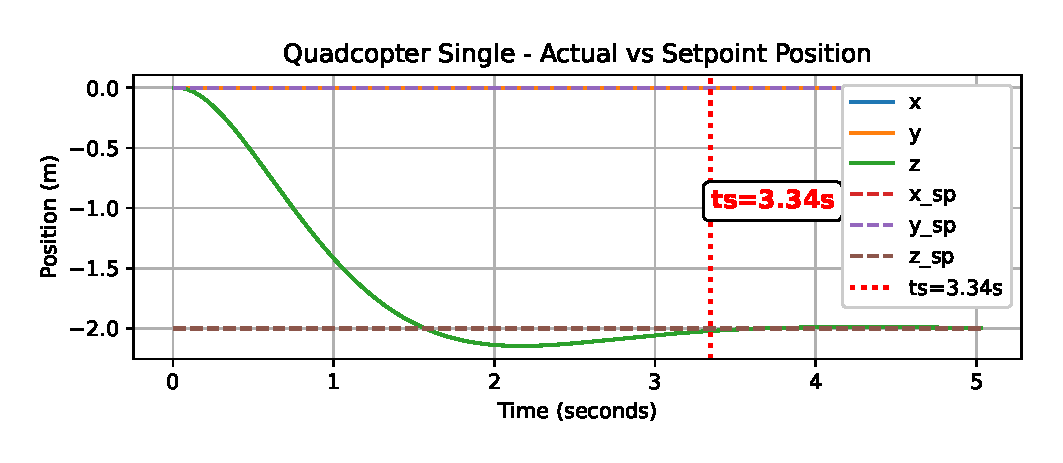
\includegraphics[width=\columnwidth]{figures/takeoff_response.eps} 
        \caption{Position tracking response during the autonomous takeoff phase. The vertical axis ($z$) successfully converges to the $-2.0$~m setpoint with a settling time of $t_s = 3.34$~s, while horizontal stability ($x, y$) is strictly maintained.}
        \label{fig:takeoff_response}
    \end{figure}

    \subsection{Scenario 1: Basic Obstacle Avoidance}
        This scenario provides a nominal baseline in a cluttered environment. Fig.~\ref{fig:basic_compare_metrics} compares the resulting trajectories and quantitative metrics for the static IAPF planner and the adaptive ERC planner.

        \begin{figure}
            \centering
            \makebox[\textwidth][c]{%
                \begin{minipage}{1.3\textwidth}
                    \centering

                    % --- KOLOM KIRI: IAPF ---
                    \begin{minipage}[t]{0.495\linewidth}
                        \centering
                        \textbf{IAPF}\\
                        \vspace{0.3em}

                        \begin{subfigure}[t]{\linewidth}
                            \centering
                            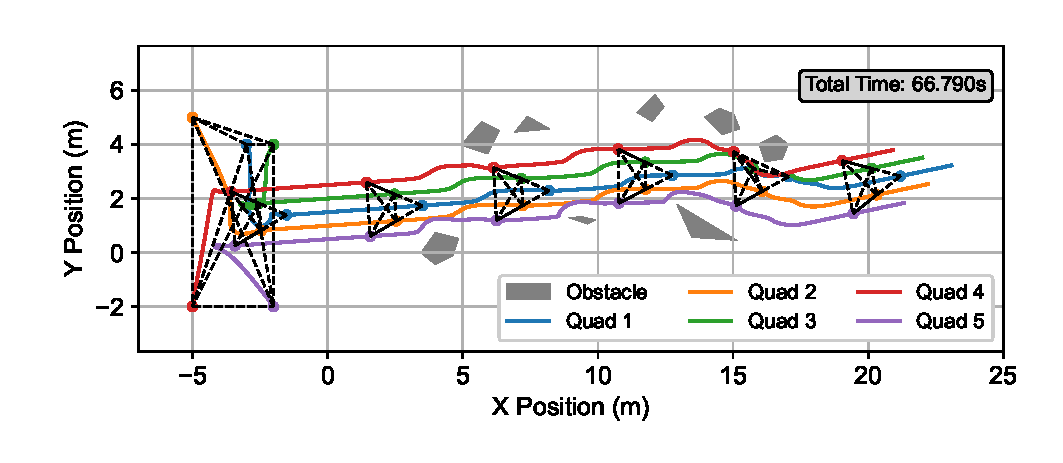
\includegraphics[width=\linewidth]{figures/iapf_basic_traj.eps}
                            \caption{Trajectory}
                            \label{fig:iapf_basic_traj}
                        \end{subfigure}
                        \hfill
                        \begin{subfigure}[t]{\linewidth}
                            \centering
                            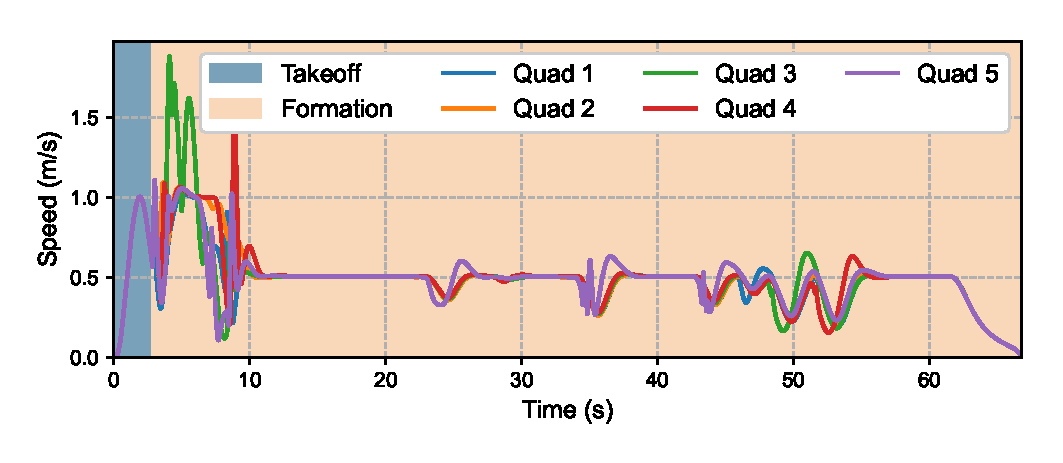
\includegraphics[width=\linewidth]{figures/iapf_basic_vel.eps}
                            \caption{Velocity}
                            \label{fig:iapf_basic_vel}
                        \end{subfigure}

                        \vspace{0.1em}

                        \begin{subfigure}[t]{\linewidth}
                            \centering
                            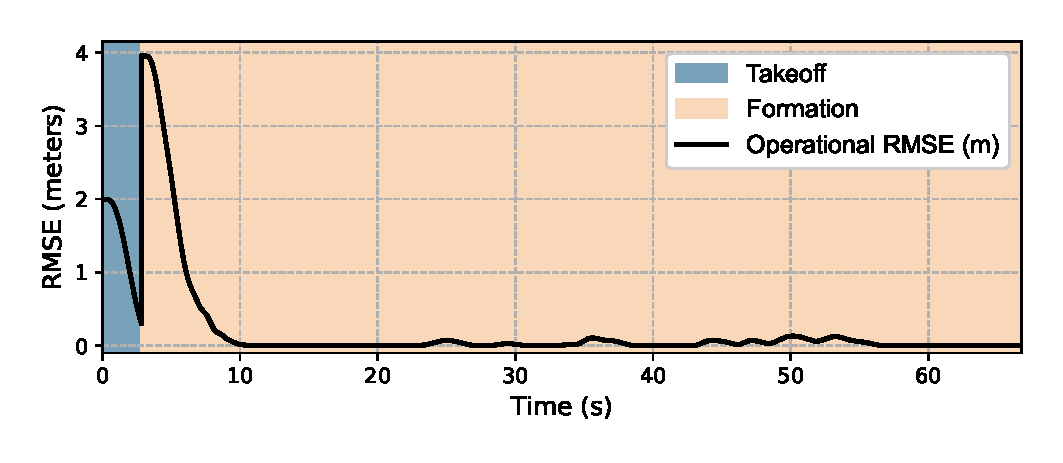
\includegraphics[width=\linewidth]{figures/iapf_basic_rmse.eps}
                            \caption{RMSE}
                            \label{fig:iapf_basic_rmse}
                        \end{subfigure}
                        \hfill
                        \begin{subfigure}[t]{\linewidth}
                            \centering
                            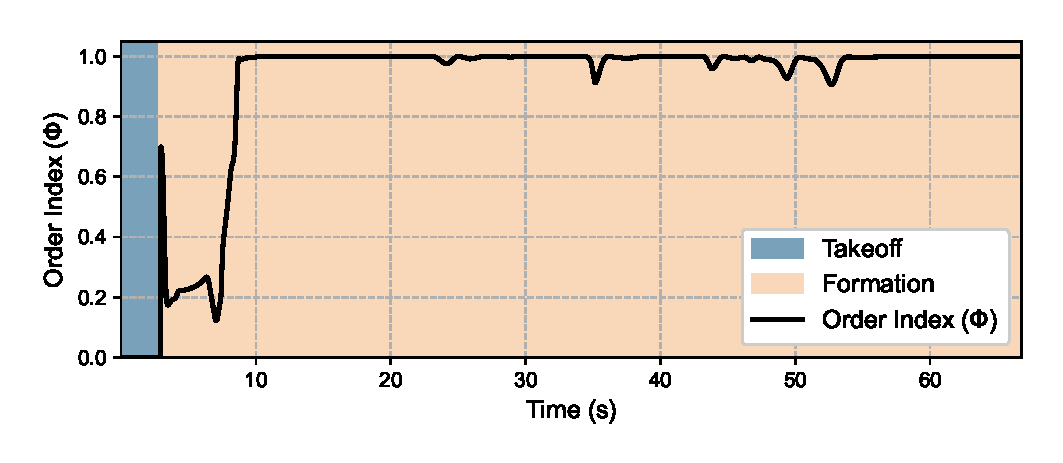
\includegraphics[width=\linewidth]{figures/iapf_basic_phi.eps}
                            \caption{$\Phi$}
                            \label{fig:iapf_basic_phi}
                        \end{subfigure}
                    \end{minipage}
                    \hfill
                    % --- KOLOM KANAN: ERC ---
                    \begin{minipage}[t]{0.495\linewidth}
                        \centering
                        \textbf{ERC}\\
                        \vspace{0.3em}

                        \begin{subfigure}[t]{\linewidth}
                            \centering
                            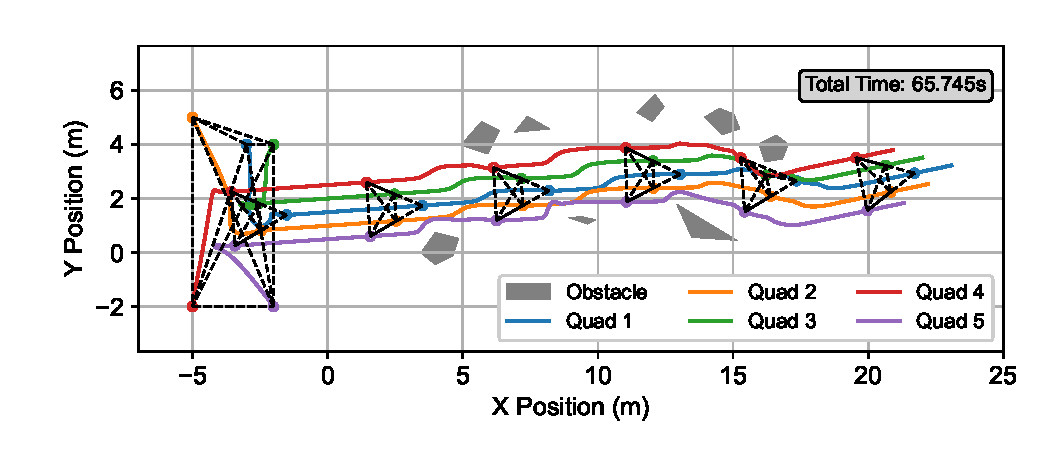
\includegraphics[width=\linewidth]{figures/erc_basic_traj.eps}
                            \caption{Trajectory}
                            \label{fig:erc_basic_traj}
                        \end{subfigure}
                        \hfill
                        \begin{subfigure}[t]{\linewidth}
                            \centering
                            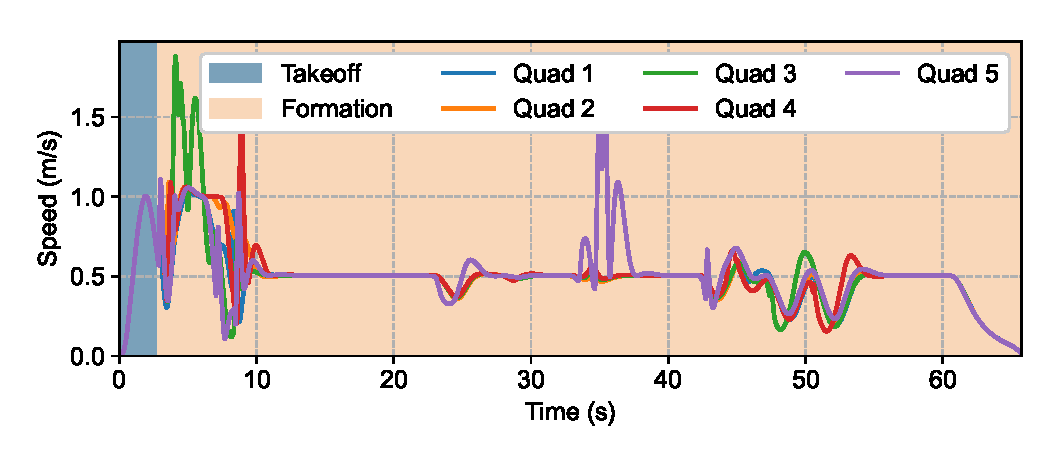
\includegraphics[width=\linewidth]{figures/erc_basic_vel.eps}
                            \caption{Velocity}
                            \label{fig:erc_basic_vel}
                        \end{subfigure}

                        \vspace{0.1em}

                        \begin{subfigure}[t]{\linewidth}
                            \centering
                            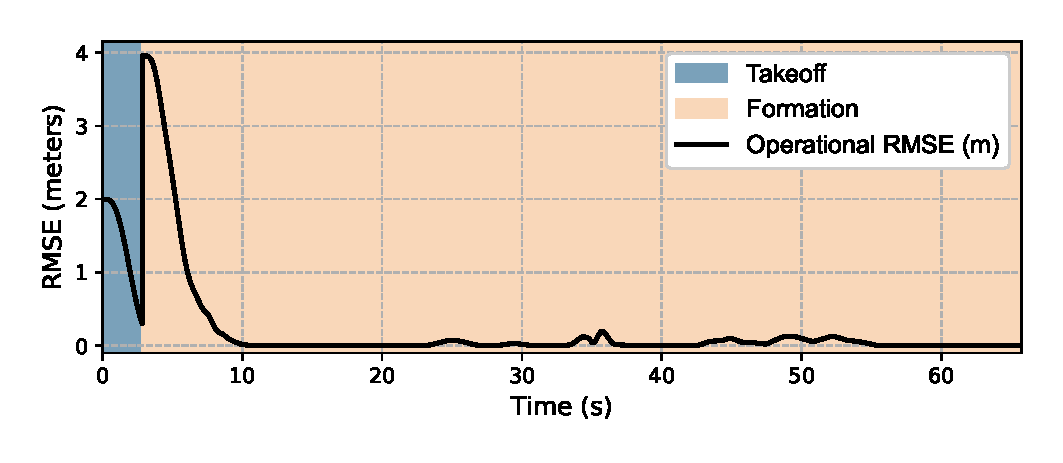
\includegraphics[width=\linewidth]{figures/erc_basic_rmse.eps}
                            \caption{RMSE}
                            \label{fig:erc_basic_rmse}
                        \end{subfigure}
                        \hfill
                        \begin{subfigure}[t]{\linewidth}
                            \centering
                            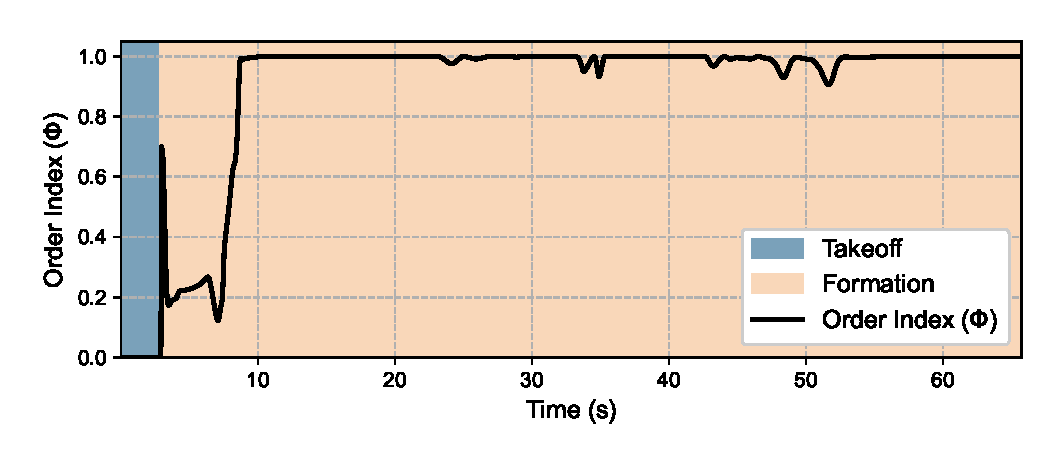
\includegraphics[width=\linewidth]{figures/erc_basic_phi.eps}
                            \caption{$\Phi$}
                            \label{fig:erc_basic_phi}
                        \end{subfigure}
                    \end{minipage}
                \end{minipage}%
            }

            \caption{Scenario 1 (basic obstacle avoidance): IAPF vs. ERC comparison. The left column reports the IAPF trajectory and metrics, while the right column reports the corresponding results for ERC.}
            \label{fig:basic_compare_metrics}
        \end{figure}

        Fig.~\ref{fig:basic_compare_metrics} shows that both planners produce smooth, collision-free trajectories in the cluttered environment. The IAPF velocity profile (Fig.~\ref{fig:iapf_basic_vel}) remains close to the migration reference except for brief avoidance-induced fluctuations, while the RMSE response (Fig.~\ref{fig:iapf_basic_rmse}) settles after the initial transient and the orderliness index stays high (Fig.~\ref{fig:iapf_basic_phi}). The ERC results in the right column exhibit comparable behavior under the same conditions.

    \subsection{Scenario 2: Narrow Gap Passage -- IAPF vs. ERC}
        This scenario stresses the planners in a constrained passage. Fig.~\ref{fig:narrow_compare_metrics} summarizes the resulting trajectories and performance metrics for IAPF and ERC.

        \begin{figure}
            \centering
            \makebox[\textwidth][c]{%
                \begin{minipage}{1.3\textwidth}
                    \centering

                    % --- KOLOM KIRI: IAPF ---
                    \begin{minipage}[t]{0.495\linewidth}
                        \centering
                        \textbf{IAPF}\\
                        \vspace{0.3em}

                        \begin{subfigure}[t]{\linewidth}
                            \centering
                            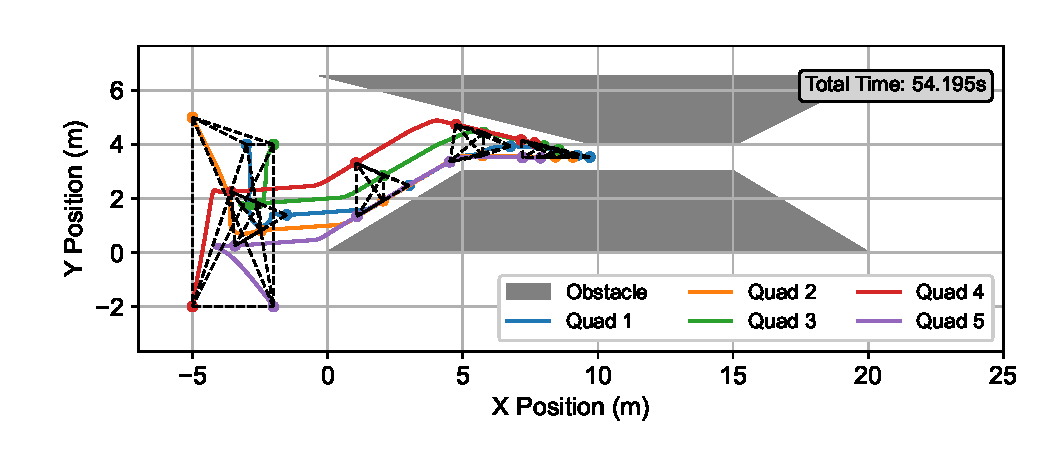
\includegraphics[width=\linewidth]{figures/iapf_narrow_fail.eps}
                            \caption{Trajectory}
                            \label{fig:iapf_narrow_fail}
                        \end{subfigure}
                        \hfill
                        % NOTE: placeholder plots (replace with IAPF outputs)
                        \begin{subfigure}[t]{\linewidth}
                            \centering
                            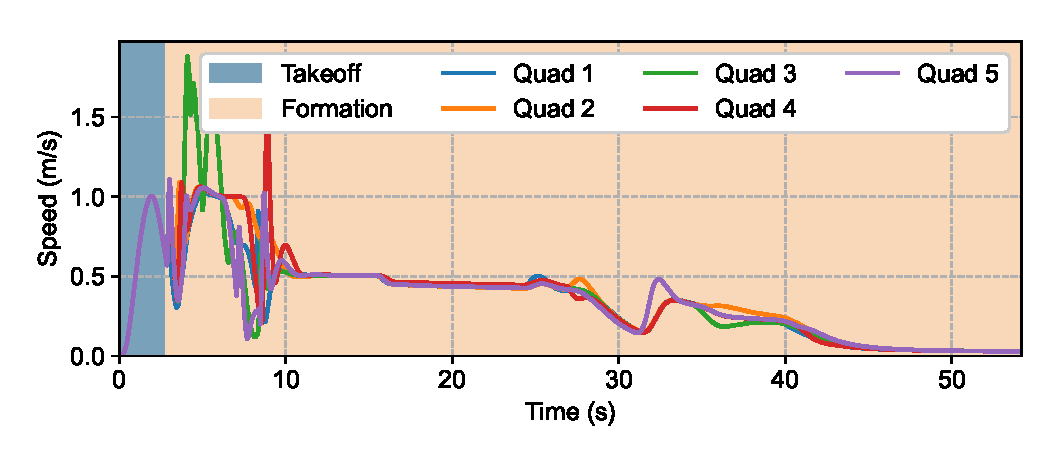
\includegraphics[width=\linewidth]{figures/iapf_narrow_vel.eps}
                            \caption{Velocity}
                            \label{fig:iapf_narrow_vel}
                        \end{subfigure}

                        \vspace{0.1em}

                        \begin{subfigure}[t]{\linewidth}
                            \centering
                            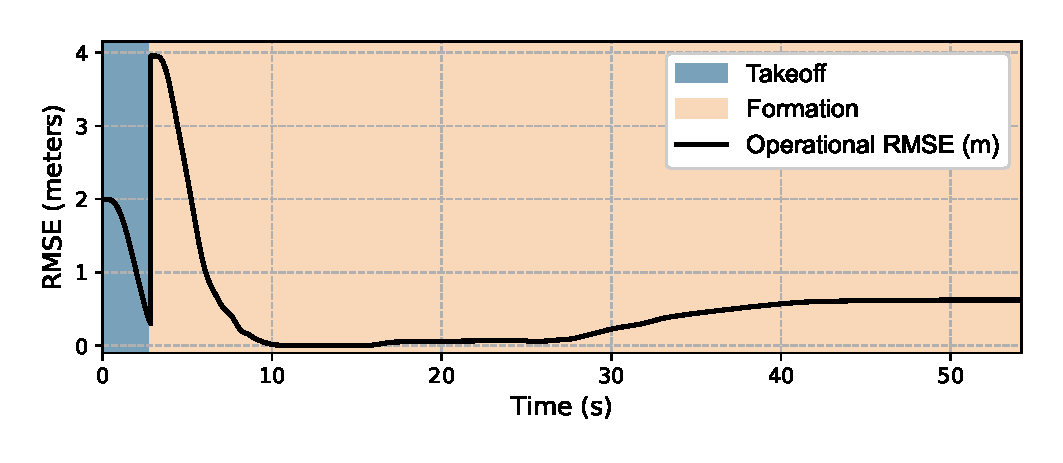
\includegraphics[width=\linewidth]{figures/iapf_narrow_rmse.eps}
                            \caption{RMSE}
                            \label{fig:iapf_narrow_rmse}
                        \end{subfigure}
                        \hfill
                        \begin{subfigure}[t]{\linewidth}
                            \centering
                            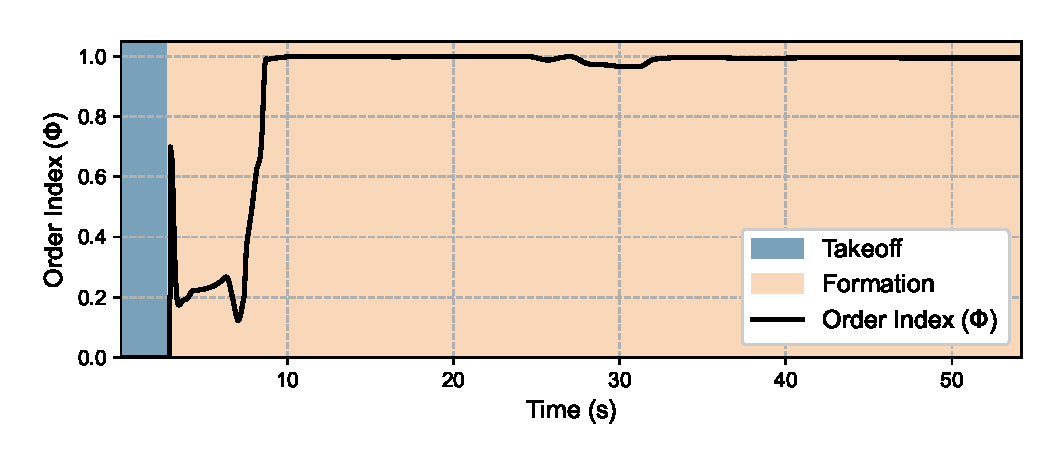
\includegraphics[width=\linewidth]{figures/iapf_narrow_phi.eps}
                            \caption{$\Phi$}
                            \label{fig:iapf_narrow_phi}
                        \end{subfigure}
                    \end{minipage}
                    \hfill
                    % --- KOLOM KANAN: ERC ---
                    \begin{minipage}[t]{0.495\linewidth}
                        \centering
                        \textbf{ERC}\\
                        \vspace{0.3em}

                        \begin{subfigure}[t]{\linewidth}
                            \centering
                            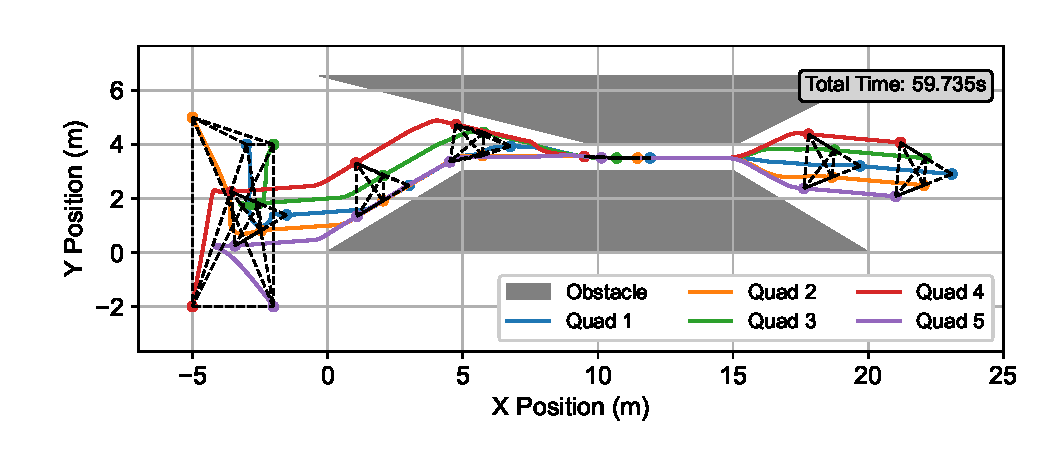
\includegraphics[width=\linewidth]{figures/erc_narrow_traj.eps}
                            \caption{Trajectory}
                            \label{fig:erc_narrow_traj}
                        \end{subfigure}
                        \hfill
                        \begin{subfigure}[t]{\linewidth}
                            \centering
                            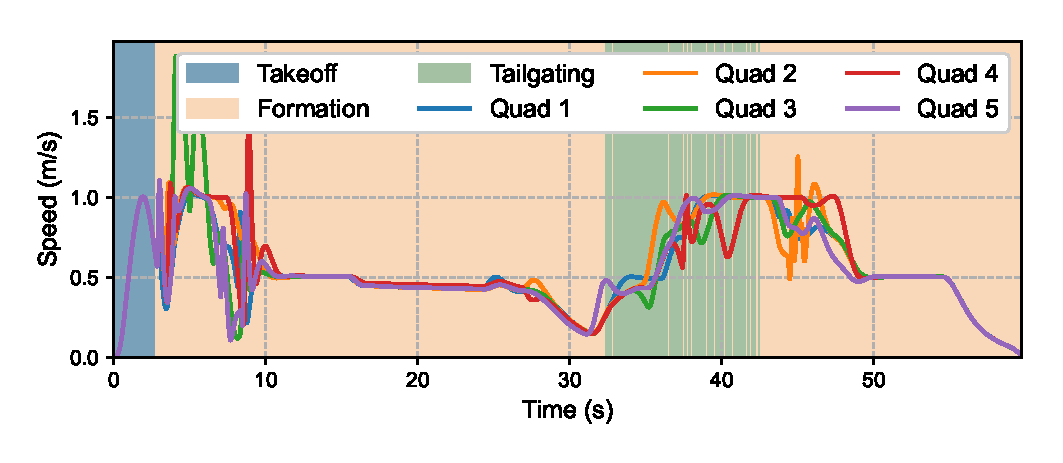
\includegraphics[width=\linewidth]{figures/erc_narrow_vel.eps}
                            \caption{Velocity}
                            \label{fig:erc_narrow_vel}
                        \end{subfigure}

                        \vspace{0.1em}

                        \begin{subfigure}[t]{\linewidth}
                            \centering
                            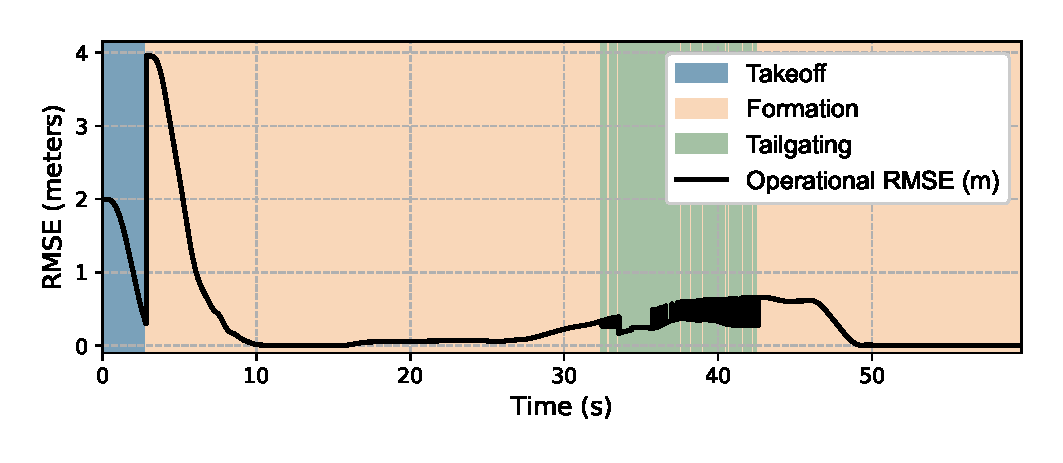
\includegraphics[width=\linewidth]{figures/erc_narrow_rmse.eps}
                            \caption{RMSE}
                            \label{fig:erc_narrow_rmse}
                        \end{subfigure}
                        \hfill
                        \begin{subfigure}[t]{\linewidth}
                            \centering
                            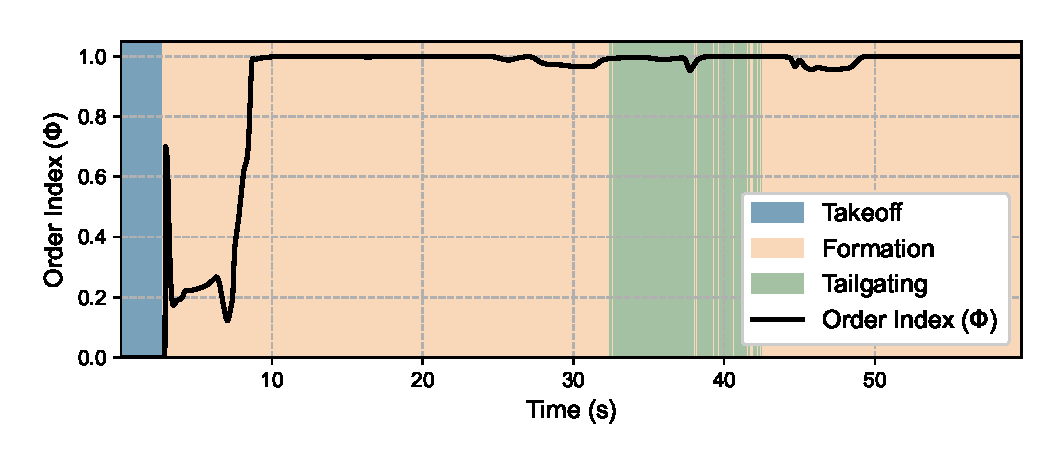
\includegraphics[width=\linewidth]{figures/erc_narrow_phi.eps}
                            \caption{$\Phi$}
                            \label{fig:erc_narrow_phi}
                        \end{subfigure}
                    \end{minipage}
                \end{minipage}%
            }

            \caption{Scenario 2 (narrow gap passage): IAPF vs. ERC comparison. The left column reports the IAPF trajectory and metrics, while the right column reports the corresponding results for ERC.}
            \label{fig:narrow_compare_metrics}
        \end{figure}

        Under IAPF, the swarm becomes trapped at the entrance and fails to traverse the passage (Fig.~\ref{fig:iapf_narrow_fail}). In contrast, ERC successfully reconfigures into a single-file structure to pass through the gap and subsequently restores the nominal formation (Fig.~\ref{fig:erc_narrow_traj}). The mode transition is visible in the velocity, RMSE, and orderliness traces (Figs.~\ref{fig:erc_narrow_vel}--\ref{fig:erc_narrow_phi}); a quantitative summary of completion time and average metrics is provided in Table~\ref{tab:compare_iapf_erc}.

        The detailed interpretation of Fig.~\ref{fig:erc_mode_switch} is deferred to the comparative analysis in Section~\ref{sec:analysis_comparison}.

    \subsection{Scenario 3: Robustness Against Wind Disturbance}
        This scenario evaluates robustness of the integrated controller under external disturbances. The applied gust profile is shown in Fig.~\ref{fig:wind_model}, and the resulting trajectory and performance metrics are summarized in Fig.~\ref{fig:erc_wind_metrics}.

        \begin{figure}
            \centering
            \makebox[\textwidth][c]{%
                \begin{minipage}{1.3\textwidth}
                    \centering

                    % --- BARIS ATAS (a, b) ---
                    \begin{subfigure}[b]{0.495\linewidth}
                        \centering
                        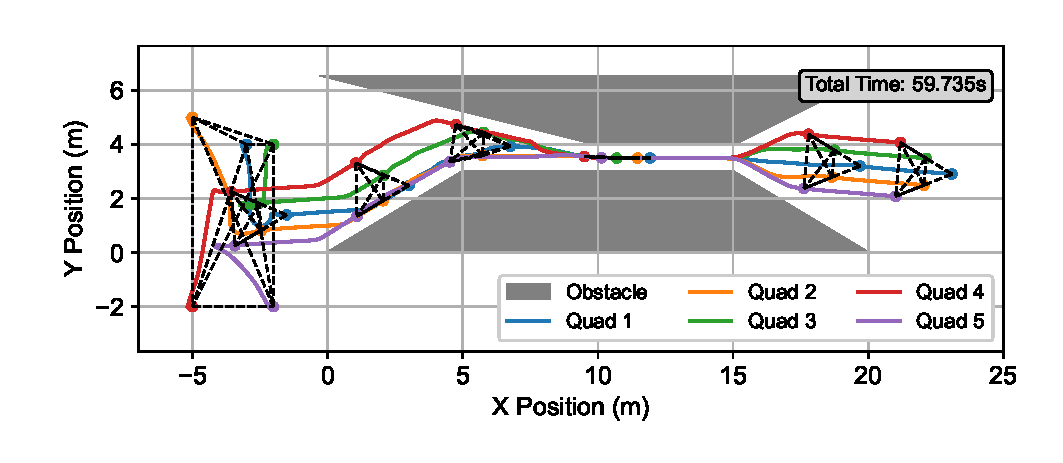
\includegraphics[width=\linewidth]{figures/erc_wind_traj.eps}
                        \caption{Swarm trajectory}
                        \label{fig:erc_wind_traj}
                    \end{subfigure}
                    \hfill
                    \begin{subfigure}[b]{0.495\linewidth}
                        \centering
                        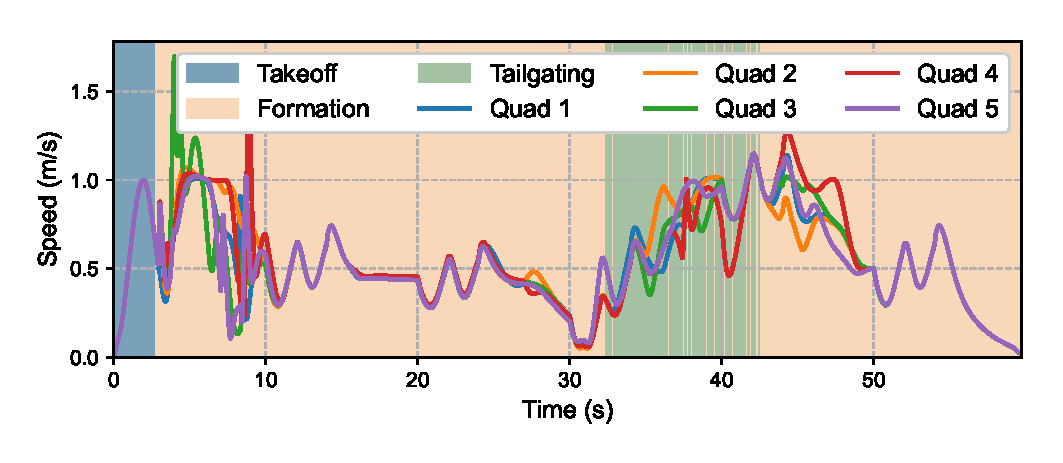
\includegraphics[width=\linewidth]{figures/erc_wind_vel.eps}
                        \caption{Swarm velocity profile}
                        \label{fig:erc_wind_vel}
                    \end{subfigure}

                    \vspace{0.1em}

                    % --- BARIS BAWAH (c, d) ---
                    \begin{subfigure}[b]{0.495\linewidth}
                        \centering
                        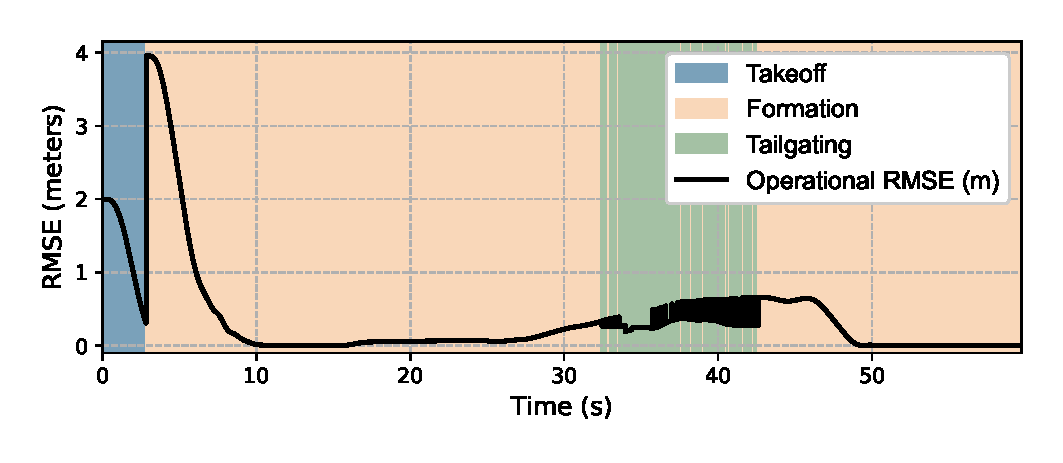
\includegraphics[width=\linewidth]{figures/erc_wind_rmse.eps}
                        \caption{Operational accuracy (RMSE)}
                        \label{fig:erc_wind_rmse}
                    \end{subfigure}
                    \hfill
                    \begin{subfigure}[b]{0.495\linewidth}
                        \centering
                        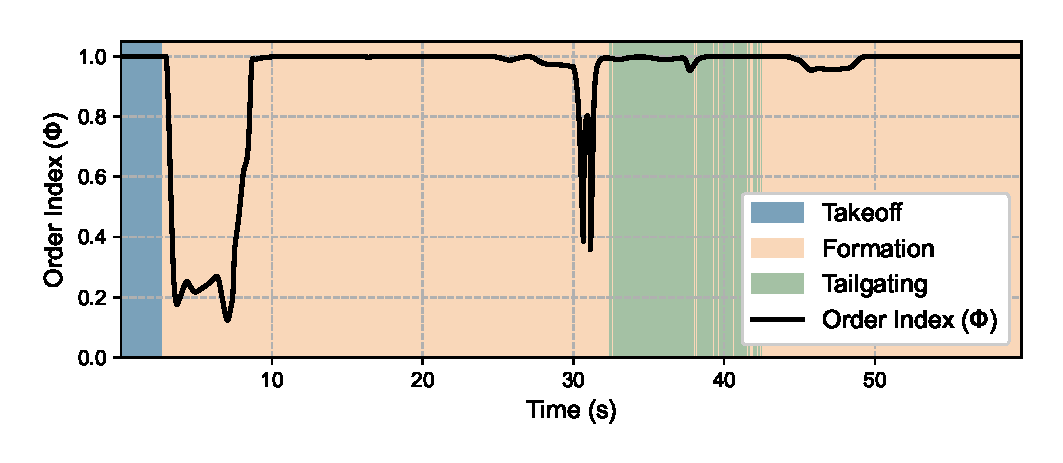
\includegraphics[width=\linewidth]{figures/erc_wind_phi.eps}
                        \caption{Motion cohesiveness ($\Phi$)}
                        \label{fig:erc_wind_phi}
                    \end{subfigure}
                \end{minipage}%
            }

            \caption{Performance of the adaptive ERC strategy in the narrow-gap scenario under external wind disturbance. (a) The swarm successfully completes the mission with a nearly identical trajectory. The quantitative metrics show (b) a velocity profile with oscillations corresponding to wind gusts, yet (c) maintained high accuracy and (d) strong cohesiveness.}
            \label{fig:erc_wind_metrics}
        \end{figure}

        Fig.~\ref{fig:erc_wind_metrics} shows that the ERC strategy preserves the intended high-level behavior during the gust interval. The trajectory remains consistent with the nominal passage (Fig.~\ref{fig:erc_wind_traj}), while the wind input induces periodic oscillations in the swarm speed (Fig.~\ref{fig:erc_wind_vel}). Despite these oscillations, the operational accuracy and motion cohesiveness remain stable, as indicated by the bounded RMSE trace (Fig.~\ref{fig:erc_wind_rmse}) and sustained high orderliness index (Fig.~\ref{fig:erc_wind_phi}). The corresponding increase in stabilization demand is discussed via the controller-effort profile in Fig.~\ref{fig:erc_wind_effort}.

    \subsection{Scenario 4: Planner Limitation Test in a Topological Trap}
        This scenario highlights a limitation of the purely reactive high-level planner in a concave (U-shaped) environment. Fig.~\ref{fig:utrap_metrics} summarizes the resulting behavior and the associated performance metrics.

        \begin{figure}
            \centering
            \makebox[\textwidth][c]{%
                \begin{minipage}{1.3\textwidth}
                    \centering

                    % --- BARIS ATAS (a, b) ---
                    \begin{subfigure}[b]{0.495\linewidth}
                        \centering
                        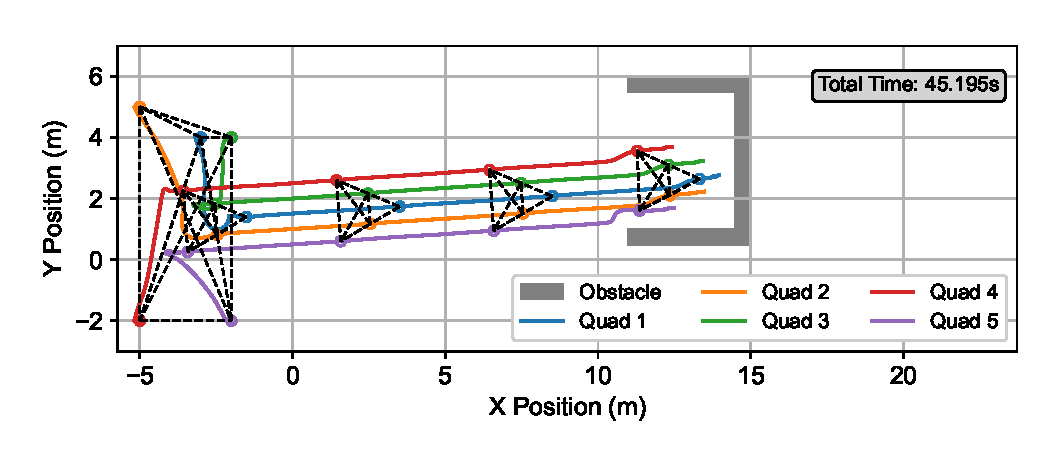
\includegraphics[width=\linewidth]{figures/utrap_fail.eps}
                        \caption{Swarm trajectory (U-Trap)}
                        \label{fig:utrap_fail}
                    \end{subfigure}
                    \hfill
                    \begin{subfigure}[b]{0.495\linewidth}
                        \centering
                        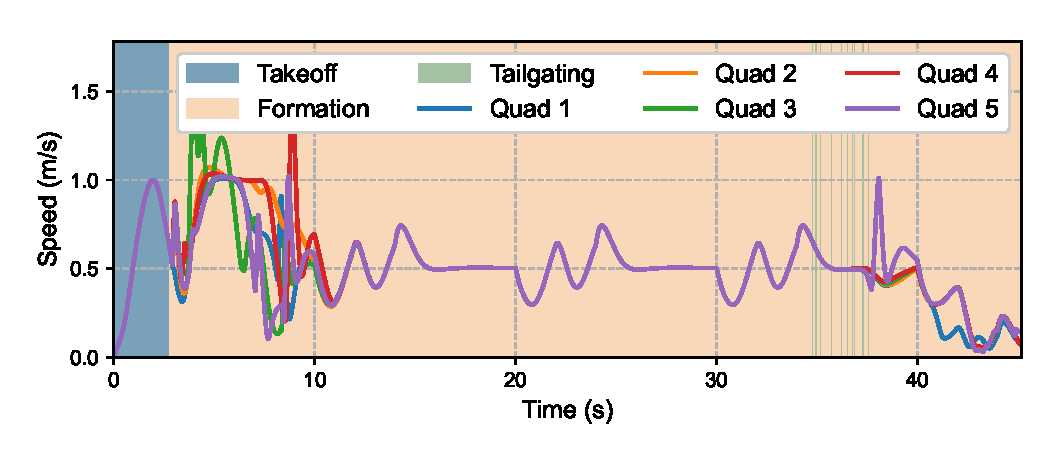
\includegraphics[width=\linewidth]{figures/utrap_vel.eps}
                        \caption{Swarm velocity profile}
                        \label{fig:utrap_vel}
                    \end{subfigure}

                    \vspace{0.1em}

                    % --- BARIS BAWAH (c, d) ---
                    \begin{subfigure}[b]{0.495\linewidth}
                        \centering
                        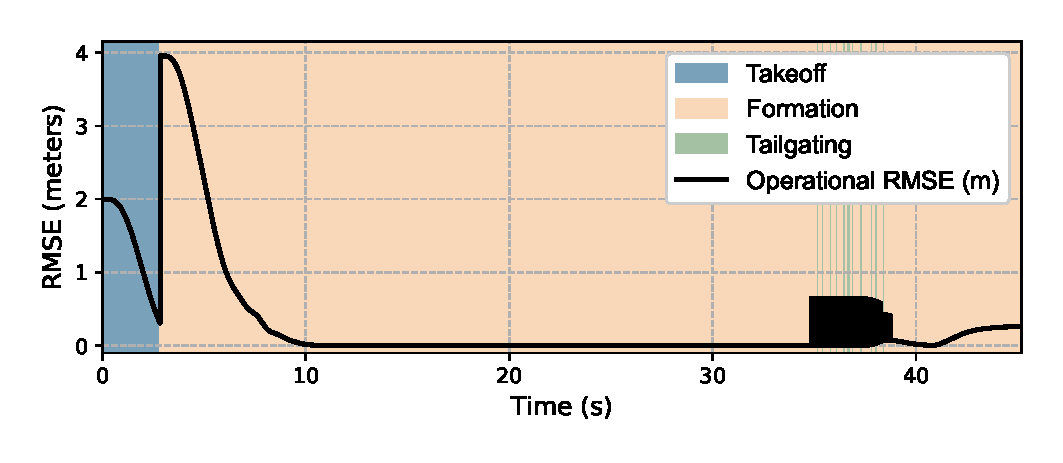
\includegraphics[width=\linewidth]{figures/utrap_rmse.eps}
                        \caption{Operational accuracy (RMSE)}
                        \label{fig:utrap_rmse}
                    \end{subfigure}
                    \hfill
                    \begin{subfigure}[b]{0.495\linewidth}
                        \centering
                        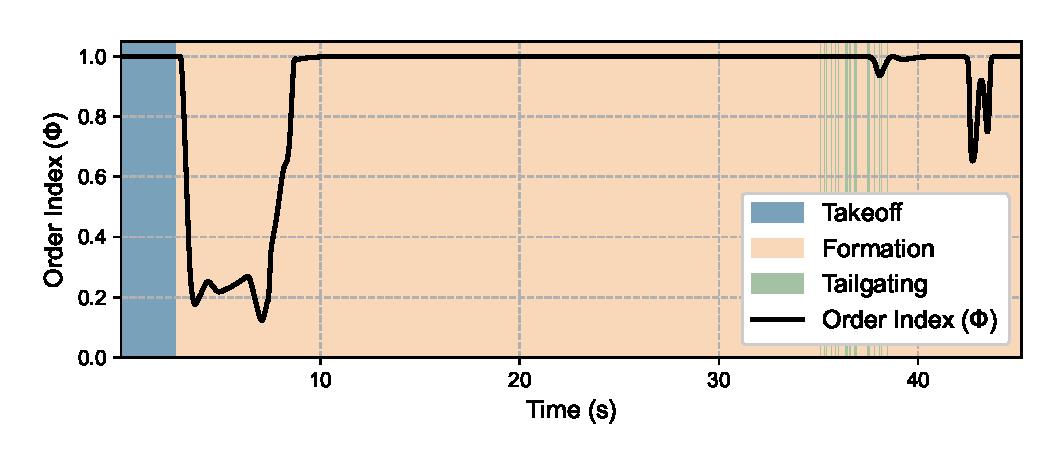
\includegraphics[width=\linewidth]{figures/utrap_phi.eps}
                        \caption{Motion cohesiveness ($\Phi$)}
                        \label{fig:utrap_phi}
                    \end{subfigure}
                \end{minipage}%
            }

            \caption{Planner limitation in the U-Trap scenario. The swarm becomes trapped in a local minimum and fails to reach the goal.}
            \label{fig:utrap_metrics}
        \end{figure}

        The trajectory in Fig.~\ref{fig:utrap_fail} shows that the swarm can enter the trap but does not escape, eventually stalling near the concave boundary. This loss of progress is reflected by the velocity decay toward zero in Fig.~\ref{fig:utrap_vel}.

        The operational accuracy (Fig.~\ref{fig:utrap_rmse}) does not converge to a goal-reaching regime and instead plateaus as the swarm hovers, while the orderliness index (Fig.~\ref{fig:utrap_phi}) remains bounded, showing that coordinated motion can be maintained even when global progress is lost. The underlying cause of this failure mode and its implications for reactive planners are discussed in Section~\ref{sec:analysis_limitations}.

    \subsection{Scenario 5: Waypoint Navigation}
        This scenario evaluates the extended planner on a multi-goal mission. The resulting $x$--$y$ trajectory and performance metrics are summarized in Fig.~\ref{fig:waypoint_metrics}.

        \begin{figure}
            \centering
            \makebox[\textwidth][c]{%
                \begin{minipage}{1.1\textwidth}
                    \centering

                    % --- DUA KOLOM: kiri 1 gambar, kanan 3 baris ---
                    \begin{minipage}[t][0.6\textheight][c]{0.40\linewidth}
                        \vspace{0pt}
                        \centering
                        \begin{subfigure}[t]{\linewidth}
                            \centering
                            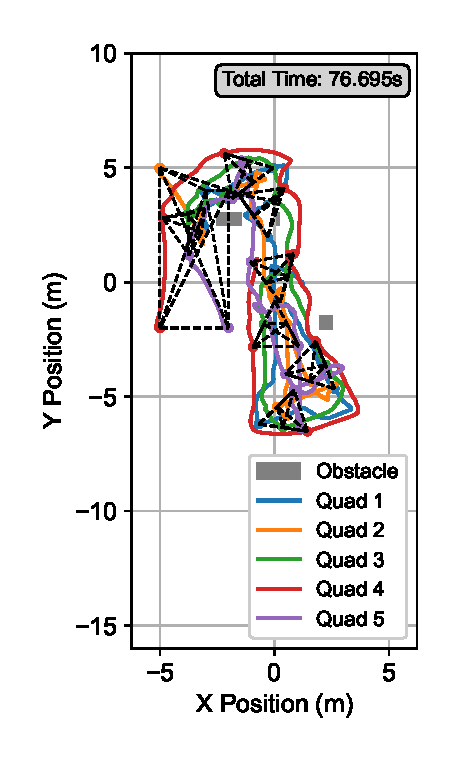
\includegraphics[width=\linewidth]{figures/waypoint_traj.eps}
                            \caption{Swarm trajectory through five waypoints}
                            \label{fig:waypoint_traj}
                        \end{subfigure}
                    \end{minipage}
                    \hfill
                    \begin{minipage}[t]{0.58\linewidth}
                        \vspace{0pt}
                        \centering
                        \begin{subfigure}[t]{\linewidth}
                            \centering
                            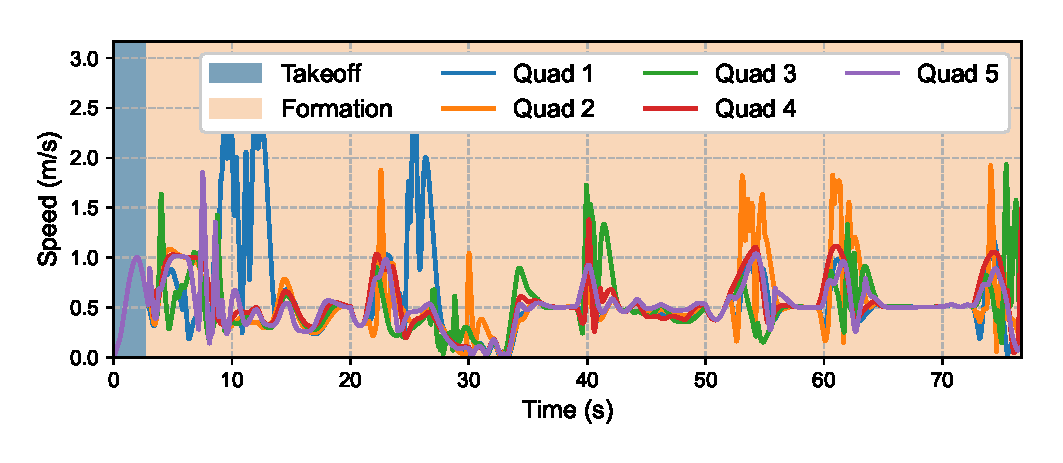
\includegraphics[width=\linewidth,height=0.22\textheight,keepaspectratio]{figures/waypoint_vel.eps}
                            \caption{Swarm velocity profile}
                            \label{fig:waypoint_vel}
                        \end{subfigure}

                        \vspace{-0.5em}

                        \begin{subfigure}[t]{\linewidth}
                            \centering
                            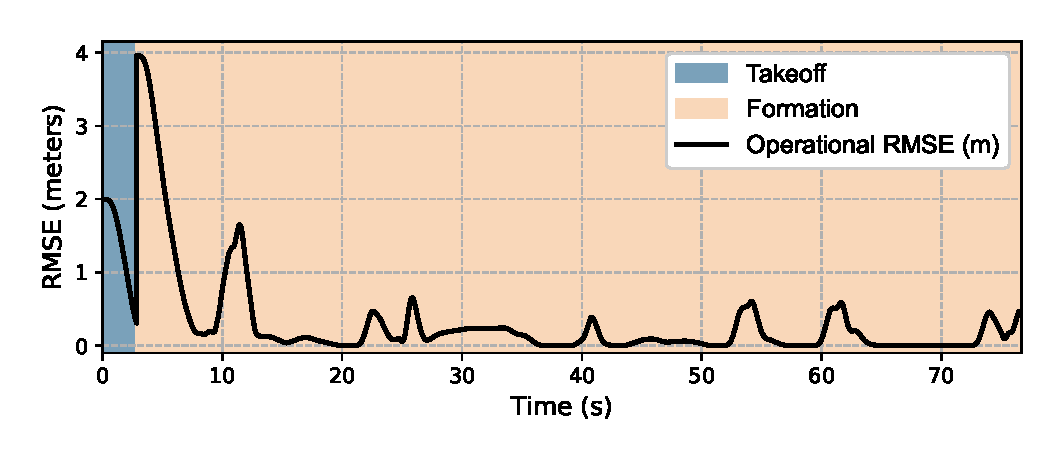
\includegraphics[width=\linewidth,height=0.22\textheight,keepaspectratio]{figures/waypoint_rmse.eps}
                            \caption{Operational accuracy (RMSE)}
                            \label{fig:waypoint_rmse}
                        \end{subfigure}

                        \vspace{-0.5em}

                        \begin{subfigure}[t]{\linewidth}
                            \centering
                            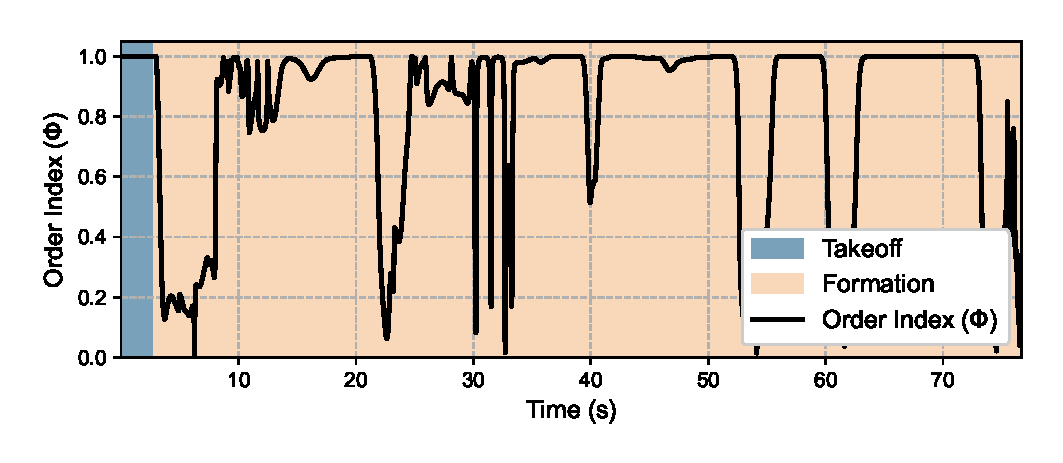
\includegraphics[width=\linewidth,height=0.22\textheight,keepaspectratio]{figures/waypoint_phi.eps}
                            \caption{Motion cohesiveness ($\Phi$)}
                            \label{fig:waypoint_phi}
                        \end{subfigure}
                    \end{minipage}
                \end{minipage}%
            }

            \caption{Performance of the ERC strategy in the waypoint navigation scenario with wind disturbance. (a) The swarm successfully navigates the complex path. The metrics show (b) a dynamic velocity profile, (c) high overall accuracy despite fluctuations during maneuvers, and (d) strong motion cohesiveness.}
            \label{fig:waypoint_metrics}
        \end{figure}

        Fig.~\ref{fig:waypoint_metrics} shows that the extended planner can execute a multi-goal waypoint mission under wind disturbance while maintaining coordinated swarm behavior. The trajectory in Fig.~\ref{fig:waypoint_traj} exhibits clear segment-by-segment progression through the waypoints with smooth transitions between legs.

        The waypoint turns induce deliberate speed modulation, visible in the oscillatory velocity profile in Fig.~\ref{fig:waypoint_vel}. These maneuvers also produce transient tracking degradations: the RMSE trace in Fig.~\ref{fig:waypoint_rmse} shows short peaks during reorientation, but repeatedly returns toward its pre-maneuver level once the swarm aligns with the next segment. Throughout the mission, the orderliness index remains bounded with only minor fluctuations (Fig.~\ref{fig:waypoint_phi}), indicating that formation coordination is preserved even during the turning events.

    \subsection{Scenario 6: Circular Path Tracking}
        The circular-tracking case evaluates performance on a continuous nonlinear reference. The resulting trajectory and metrics are shown in Fig.~\ref{fig:circle_metrics}.

        \begin{figure}
            \centering
            \makebox[\textwidth][c]{%
                \begin{minipage}{1.3\textwidth}
                    \centering

                    % --- BARIS ATAS (a, b) ---
                    \begin{subfigure}[b]{0.495\linewidth}
                        \centering
                        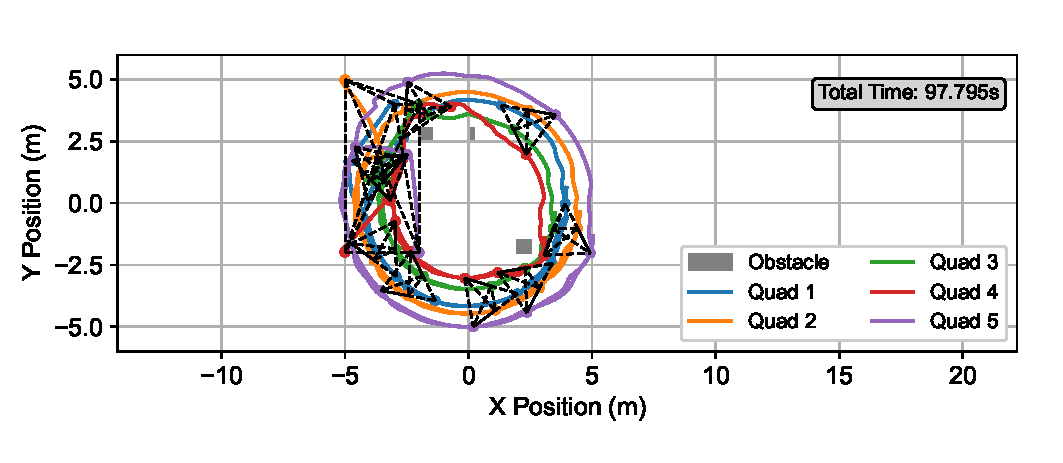
\includegraphics[width=\linewidth]{figures/circle_traj.eps} 
                        \caption{Swarm trajectory on a circular path}
                        \label{fig:circle_traj}
                    \end{subfigure}
                    \hfill
                    \begin{subfigure}[b]{0.495\linewidth}
                        \centering
                        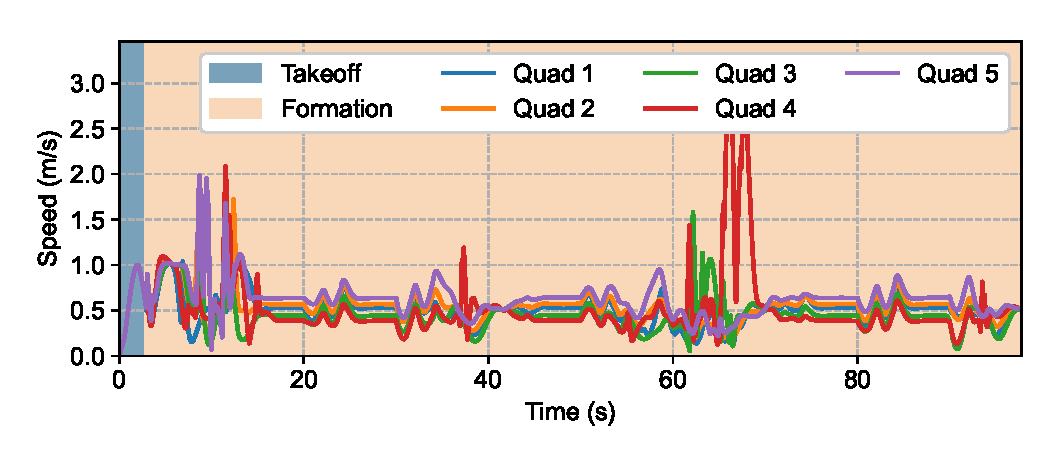
\includegraphics[width=\linewidth]{figures/circle_vel.eps} 
                        \caption{Swarm velocity profile}
                        \label{fig:circle_vel}
                    \end{subfigure}

                    \vspace{0.1em} 

                    % --- BARIS BAWAH (c, d) ---
                    \begin{subfigure}[b]{0.495\linewidth}
                        \centering
                        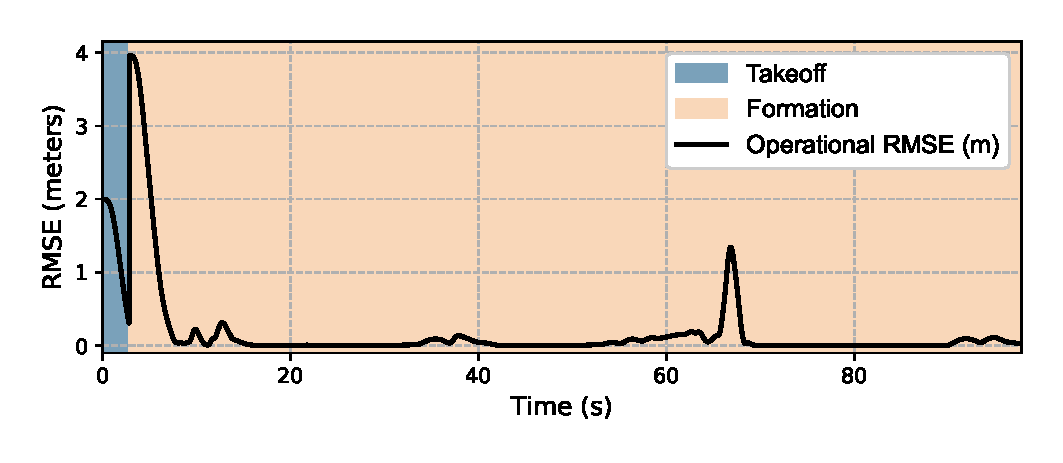
\includegraphics[width=\linewidth]{figures/circle_rmse.eps}
                        \caption{Operational accuracy (RMSE)}
                        \label{fig:circle_rmse}
                    \end{subfigure}
                    \hfill
                    \begin{subfigure}[b]{0.495\linewidth}
                        \centering
                        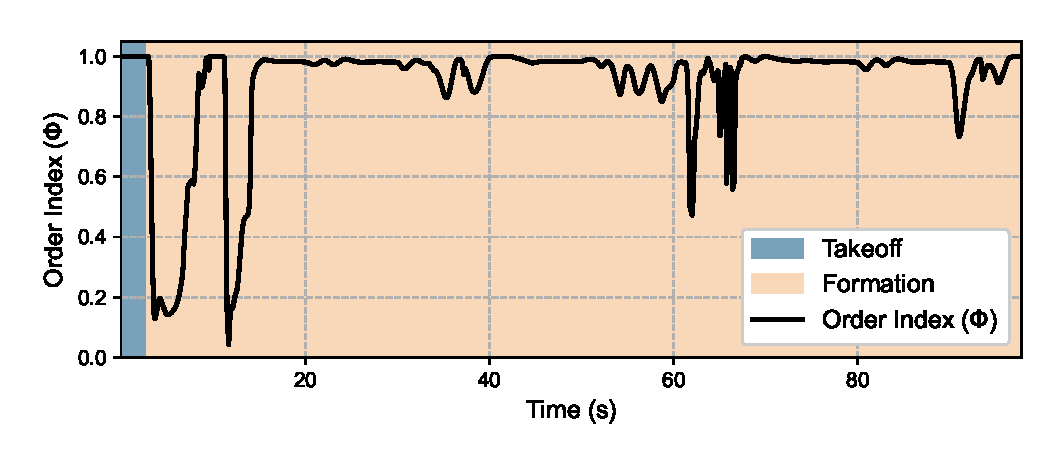
\includegraphics[width=\linewidth]{figures/circle_phi.eps} 
                        \caption{Motion cohesiveness ($\Phi$)}
                        \label{fig:circle_phi}
                    \end{subfigure}
                \end{minipage}%
            }

            \caption{Performance of the ERC strategy in the circular path tracking scenario. (a) The swarm tracks the nonlinear trajectory. The metrics show (b) a stable velocity profile, (c) bounded tracking error, and (d) sustained motion cohesiveness.}
            \label{fig:circle_metrics}
        \end{figure}

        Fig.~\ref{fig:circle_metrics} shows that the planner can follow a continuous nonlinear reference while maintaining a coherent formation. The trajectory in Fig.~\ref{fig:circle_traj} remains close to the desired circular path, and the velocity profile in Fig.~\ref{fig:circle_vel} stays smooth without large oscillations.

        The RMSE trace in Fig.~\ref{fig:circle_rmse} remains bounded throughout the maneuver, indicating consistent tracking performance along the full cycle. Motion cohesiveness is likewise sustained (Fig.~\ref{fig:circle_phi}), showing that the agents preserve coordinated motion while traversing the curved reference.

\section{Discussion and Analysis}
    This section synthesizes the scenario-based results with a clearer question-driven structure. Specifically, it addresses four points: (i) whether ERC preserves nominal performance while improving constrained-space feasibility, (ii) how robust the framework is under wind disturbance, (iii) what failure mode appears in topological traps, and (iv) whether the proposed planner extensions support more complex navigation tasks.

    \subsection{Comparative Performance: IAPF vs. ERC} \label{sec:analysis_comparison}

        To complement the trajectory results, Table~\ref{tab:compare_iapf_erc} summarizes the mission outcomes and average performance metrics for IAPF and ERC in Scenarios~1--2. This comparison evaluates whether the ERC adaptive mechanism maintains nominal performance in unconstrained environments (Scenario~1) and whether it provides a measurable advantage in constrained passages (Scenario~2).

        \begin{table*}
            \centering
            \caption{Comparison of IAPF and ERC across Scenarios 1--2.}
            \label{tab:compare_iapf_erc}
            \small

            \makebox[\textwidth][c]{%
                \begin{minipage}{1.3\textwidth}
                    \centering
                    \begin{tabular}{c c c c c c c c c c c}
                        \toprule
                        \multirow{2}{*}{\textbf{Scenario}} & \multicolumn{2}{c}{\textbf{Outcome}} & \multicolumn{2}{c}{\textbf{Time (s)}} & \multicolumn{2}{c}{\textbf{Avg. Speed (m/s)}} & \multicolumn{2}{c}{$\boldsymbol{\overline{RMSE}_{\text{total}}}$ \textbf{(m)}} & \multicolumn{2}{c}{$\boldsymbol{\overline{\Phi}}$ \textbf{(-)}} \\
                        \cmidrule(lr){2-3}\cmidrule(lr){4-5}\cmidrule(lr){6-7}\cmidrule(lr){8-9}\cmidrule(lr){10-11}
                        & \textbf{IAPF} & \textbf{ERC} & \textbf{IAPF} & \textbf{ERC} & \textbf{IAPF} & \textbf{ERC} & \textbf{IAPF} & \textbf{ERC} & \textbf{IAPF} & \textbf{ERC} \\
                        \midrule
                        1 & Success & Success & 66.790 & \textbf{65.745} & 0.492 & \textbf{0.503} & \textbf{0.236} & 0.241 & \textbf{0.892} & 0.890 \\
                        2 & Fail & Success & 54.195 & \textbf{59.735} & 0.365 & \textbf{0.561} & 0.525 & \textbf{0.692} & 0.868 & \textbf{0.878} \\
                        \bottomrule
                    \end{tabular}
                \end{minipage}%
            }
        \end{table*}

        In the baseline cluttered environment (Scenario~1), both planners succeed and yield comparable average metrics. ERC exhibits a slightly shorter traversal time (65.745~s vs.~66.790~s) and a proportional increase in mean speed (0.503~m/s vs.~0.492~m/s). The tracking accuracy and cohesiveness remain statistically similar ($\overline{RMSE}_{\text{total}}=0.241$~m vs.~0.236~m; $\overline{\Phi}=0.890$ vs.~0.892). This indicates that the inclusion of the adaptive reconfiguration logic does not impose a computational or kinematic penalty in unconstrained conditions.

        In the narrow passage (Scenario~2), the operational divergence is distinct. The IAPF planner fails because the rigid formation constraints conflict with the collision-avoidance repulsion, causing the swarm to stall at the entrance. Conversely, ERC succeeds by dynamically compressing the topology and transitioning to a single-file tailgating behavior. ERC completes the mission in 59.735~s while sustaining group order ($\overline{\Phi}=0.878$). The measured increase in average tracking error ($\overline{RMSE}_{\text{total}}=0.692$~m) is a direct consequence of the intentional geometric deformation required during reconfiguration, representing a necessary mathematical trade-off to ensure spatial feasibility.

        The mechanism behind ERC's successful passage through constrained environments is illustrated by Fig.~\ref{fig:erc_mode_switch}. The plot highlights a two-tier adaptive response. First, the formation scaling factor ($\kappa$, black curve on the right axis) decreases as the swarm approaches the gap (around $t=22$ s), compressing the formation. Then, once the estimated environmental width drops below the trigger threshold, agents progressively switch from formation mode to tailgating mode (agent count on the left axis, approximately $t=32$--$44$ s), enabling a single-file reconfiguration. After clearing the passage, agents switch back to formation mode and $\kappa$ returns to 1.0, restoring the nominal topology.

        \begin{figure}
            \centering
            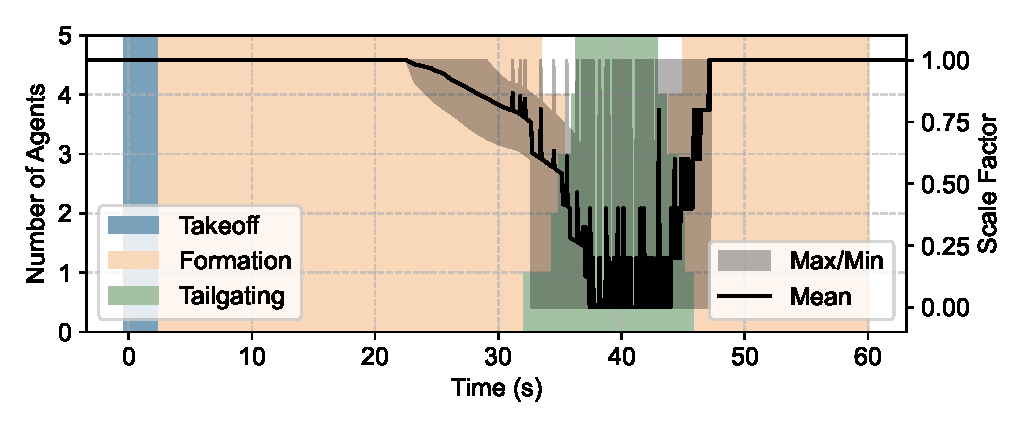
\includegraphics[width=\columnwidth]{figures/erc_mode_switch.pdf}
            \caption{Agent mode transitions and formation scaling factor ($\kappa$).}
            \label{fig:erc_mode_switch}
        \end{figure}

    \subsection{Robustness to Wind Disturbance} \label{sec:analysis_wind}

        Scenario~3 evaluates disturbance rejection by introducing periodic wind gusts during the narrow-gap passage. Table~\ref{tab:compare_erc_wind} summarizes the key performance metrics for ERC in the nominal case (no wind) and under wind disturbance.

        \begin{table*}
            \centering
            \caption{ERC robustness comparison for Scenario~3 (wind disturbance).}
            \label{tab:compare_erc_wind}
            \small

            \makebox[\textwidth][c]{%
                \begin{minipage}{1.7\textwidth}
                    \centering
                    \begin{tabular}{c c c c c c c c c c c}
                        \toprule
                        \multirow[c]{3}{*}{\textbf{Scenario}} & \multicolumn{10}{c}{\textbf{ERC}} \\
                        \cmidrule(lr){2-11}
                        & \multicolumn{2}{c}{\textbf{Outcome}} & \multicolumn{2}{c}{\textbf{Time (s)}} & \multicolumn{2}{c}{\textbf{Avg. Speed (m/s)}} & \multicolumn{2}{c}{$\boldsymbol{\overline{RMSE}_{\text{total}}}$ \textbf{(m)}} & \multicolumn{2}{c}{$\boldsymbol{\overline{\Phi}}$ \textbf{(-)}} \\
                        \cmidrule(lr){2-3}\cmidrule(lr){4-5}\cmidrule(lr){6-7}\cmidrule(lr){8-9}\cmidrule(lr){10-11}
                        & \textbf{No wind} & \textbf{Wind} & \textbf{No wind} & \textbf{Wind} & \textbf{No wind} & \textbf{Wind} & \textbf{No wind} & \textbf{Wind} & \textbf{No wind} & \textbf{Wind} \\
                        \midrule
                        3 & Success & Success & 59.735 & 59.735 & 0.561 & 0.557 & 0.692 & 0.694 & 0.878 & 0.925 \\
                        \bottomrule
                    \end{tabular}
                \end{minipage}%
            }
        \end{table*}

        As summarized in Table~\ref{tab:compare_erc_wind}, the disturbance does not prevent mission completion: both runs succeed and require the same traversal time (59.735~s). The average speed changes only slightly (0.561~m/s without wind versus 0.557~m/s with wind), indicating that migration progress is largely preserved.

        The detailed metrics reveal a nuanced system response to the aerodynamic disturbance. As expected, the external wind gusts introduce physical perturbations, causing the overall tracking error ($\overline{RMSE}_{\text{total}}$) to marginally increase from 0.692~m to 0.694~m. However, this negligible increase demonstrates the excellent disturbance rejection capabilities of the low-level cascaded PID controller, which tightly bounds the positional deviations.

        Interestingly, despite the slight drop in positional accuracy, the motion cohesiveness ($\overline{\Phi}$) actually improves from 0.878 to 0.925. This increase in orderliness is a direct aerodynamic consequence of the specific wind profile. Because the gust acts as a uniform headwind opposing the entire swarm's direction of travel, all agents must continuously and synchronously maintain a strong forward thrust to overcome it. This shared, persistent resistance essentially polarizes the swarm, dampening independent reactive micro-movements and forcing their velocity vectors to align more uniformly, resulting in a highly cohesive collective motion.

        To objectively quantify the stabilization demand required to maintain this robust behavior, we define the average control effort, $E(t)$, as the mean sum of squared commanded motor speeds across all agents in the swarm:

        \begin{equation}
            E(t) = \frac{1}{N} \sum_{i=1}^{N} \sum_{j=1}^{4} \omega_{M_{i,j}}^2(t)
        \end{equation}

        Because the aerodynamic thrust generated by each rotor is proportional to the square of its angular velocity ($T \propto \omega^2$), this metric serves as a direct surrogate for the instantaneous mechanical power and total thrust demanded by the low-level controllers.

        The impact of the aerodynamic disturbance on this metric is clearly illustrated in Fig.~\ref{fig:erc_wind_effort}. During the initial takeoff and open-space formation phases, the effort profiles for both the nominal (blue line) and wind-disturbed (red line) runs are virtually identical. However, a significant divergence occurs when the swarm enters the narrow-gap passage (indicated by the green tailgating region, $t \approx 32\text{--}42$~s). 

        \begin{figure}
            \centering
            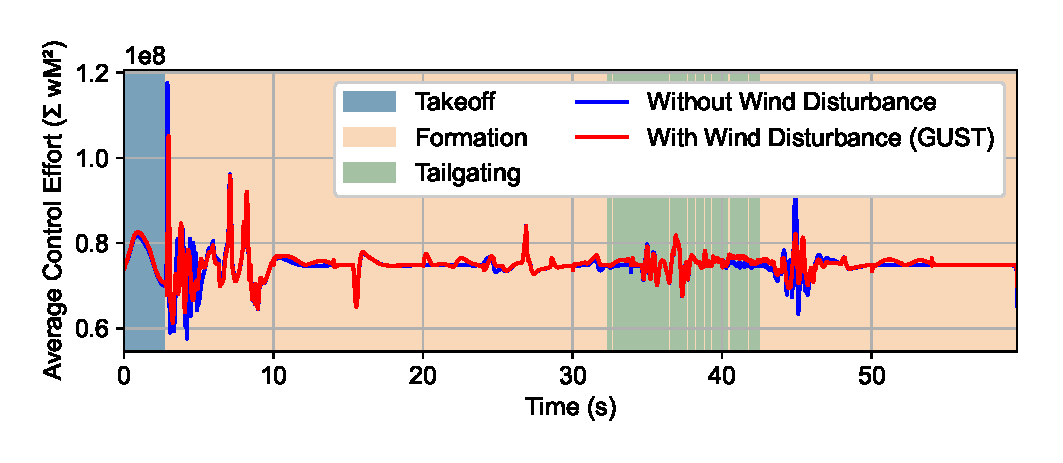
\includegraphics[width=\columnwidth]{figures/erc_wind_effort.eps}
            \caption{Controller-effort profile during the wind-gust interval in Scenario~3, illustrating the increased stabilization demand required to reject external disturbances.}
            \label{fig:erc_wind_effort}
        \end{figure}

        While the nominal run maintains a relatively smooth and baseline effort profile during this maneuver, the wind-disturbed run exhibits aggressive, high-frequency spikes. These sharp peaks perfectly coincide with the 4-second active bursts of the headwind gusts. This explicitly highlights the rapid, compensatory control actions generated by the inner PID loops; to prevent the quadcopters from being blown backward and to strictly maintain the tailgating distance ($d_{\text{ref}}$), the controllers must continually and drastically increase the motor speeds. Consequently, the tightly bounded tracking error and higher motion cohesiveness observed in the previous section come at the direct cost of significantly higher energy consumption and continuous actuator exertion.

    \subsection{System Limitations and Failure Modes} \label{sec:analysis_limitations}

        While the proposed framework demonstrates robust adaptability, navigating the transition from simulated environments to physical deployment requires acknowledging several system boundaries and theoretical assumptions.

        \textbf{Algorithmic Limitations in Topological Traps:} Scenario~4 (U-Trap) demonstrates a fundamental structural limitation of artificial potential field methodologies in concave environments. Because the high-level planner is memoryless and operates purely reactively, the migration vector is computed from the instantaneous superposition of the attractive goal force and the repulsive obstacle forces. In a U-shaped geometry, these vectors can perfectly cancel each other out before the goal is reached, creating a local minimum equilibrium. This kinematic state is confirmed by the velocity collapse shown in Fig.~\ref{fig:utrap_vel} and the horizontal plateau of the RMSE trace in Fig.~\ref{fig:utrap_rmse}. Once the swarm enters the concave boundary, the net outward command diminishes to zero. Concurrently, the cohesiveness index (Fig.~\ref{fig:utrap_phi}) remains bounded, indicating that the local formation and collision-avoidance routines maintain internal order even as global navigation fails. Resolving this limitation requires integrating non-reactive heuristics. Specifically, implementing a dedicated stagnation detector that triggers an automated escape behavior---such as a coordinated random walk or boundary wall-following---when the swarm's velocity drops below a critical threshold ($||v_{\text{ref}}|| < \epsilon_v$) would effectively complement the current reactive architecture.

        \textbf{Aerodynamic Modeling Constraints:} Beyond algorithmic constraints, a critical limitation of the current physical modeling pertains to inter-agent aerodynamic interference. While the simulation accurately models macroscopic environmental wind gusts (Scenario~3), it presently neglects localized rotor downwash effects. When quadcopters operate in highly compressed configurations---particularly the single-file tailgating mode utilized in Scenario~2---leading agents generate significant downward and rearward turbulence that inherently degrades the attitude stability of trailing followers. Future iterations of the dynamic model must incorporate downwash interference to rigorously validate the low-level controller's capacity to maintain the required tailgating distance ($d_{\text{ref}}$) under self-induced turbulent conditions.

        \textbf{State Estimation and Sim-to-Real Gap:} The current decentralized planner operates under the assumption of perfect state knowledge and instantaneous communication among the swarm. In real-world multi-quadcopter deployments, agents are inevitably subjected to sensor noise (e.g., IMU inaccuracies, GPS drift) and communication constraints (e.g., telemetry latency, packet loss). These stochastic factors can introduce phase lags into the reactive control loops. In highly constrained environments, such delays may cause oscillatory behavior in the formation-keeping vector ($\boldsymbol{v}_i^{\text{form}}$) or critically delay the collision-avoidance repulsion ($\boldsymbol{v}_i^{\text{rep}}$), potentially breaching safety margins ($r_a$). Transitioning this framework to physical platforms will inherently necessitate the integration of robust state estimators, such as Extended Kalman Filters (EKF), and delay-tolerant communication protocols.

        \textbf{Agent Failure and Chain Robustness:} In the event of a "hard stop" where a leading agent remains physically present as an obstacle, the tailgating logic combined with collision avoidance ensures safety by halting the followers. However, as demonstrated by the dynamic indexing in Section 3.5, the swarm's decentralized nature allows it to recover if an agent is entirely bypassed or removed, preventing a single point of failure from jeopardizing the entire mission.

        \textbf{Computational and Kinematic Scalability:} A final operational consideration pertains to the scalability of the framework for massive swarms (e.g., $N \ge 50$). In the current centralized simulation environment, calculating the collision-avoidance ($\boldsymbol{v}_i^{\text{rep}}$) and formation-keeping ($\boldsymbol{v}_i^{\text{form}}$) vectors requires pairwise distance checks, resulting in an $\mathcal{O}(N^2)$ computational complexity. However, because the proposed ERC architecture is fundamentally decentralized, physical deployment distributes this burden. By strictly enforcing a localized sensing radius ($r_a$), the onboard computational complexity for each quadcopter is inherently capped at $\mathcal{O}(M)$, where $M$ is the number of immediate neighbors ($M \ll N$). Kinematically, navigating a massive swarm through a narrow corridor via single-file tailgating would inevitably induce "accordion" (traffic shockwave) effects. These longitudinal compression waves would cause transient fluctuations in inter-agent distances, proportionally degrading the macroscopic orderliness index ($\overline{\Phi}$) and increasing traversal time. Evaluating these fluid-like dense swarm dynamics remains an essential objective for future large-scale investigations.

    \subsection{Extensions to Complex Navigation Tasks} \label{sec:analysis_extensions}

        Scenarios~5--6 assess the integrated navigation extensions designed to handle complex trajectories beyond linear migration. In Scenario~5, the planner successfully tracks a sequence of 3D waypoints. The trajectory (Fig.~\ref{fig:waypoint_traj}) displays controlled transitions between segments. The periodic fluctuations in speed (Fig.~\ref{fig:waypoint_vel}) and the transient spikes in RMSE (Fig.~\ref{fig:waypoint_rmse}) are direct kinematic consequences of the rotational accelerations required to reorient the entire swarm at each waypoint. Despite these directional shifts, the orderliness index ($\overline{\Phi}$) remains high (Fig.~\ref{fig:waypoint_phi}), confirming that structural coordination is not lost during sharp maneuvers.

        Scenario~6 extends this evaluation to continuous, nonlinear tracking. The circular-path data (Fig.~\ref{fig:circle_metrics}) indicates that the swarm successfully tracks the continuous reference curve without inducing large oscillatory instability in the velocity profile. The bounded RMSE trace confirms steady-state tracking performance. These results substantiate that the dynamic formation orientation and waypoint modules can be integrated into the decentralized reactive planner to execute realistic mission profiles.

    \subsection{Comparison with Prior Literature} \label{sec:comparison_literature}

        Direct quantitative comparisons with external studies are often precluded by discrepancies in UAV dynamic modeling (e.g., point-mass kinematics versus 6-DoF dynamics), environmental scales, and metric formulations. Therefore, this study employs the IAPF strategy \citep{wang_uav_2021, prabaswara_collision-free_2025} under identical simulation conditions as a rigorous baseline representing state-of-the-art static reactive planners.

        Contextualizing the proposed 3D-ERC framework against the broader literature highlights three key comparative advantages:

        \begin{itemize}
            \item \textbf{Versus Static APF/IAPF:} Traditional APF and IAPF methods \citep{khatib_real-time_1985, wang_uav_2021, prabaswara_collision-free_2025} are well-suited for scattered obstacle fields (Scenario~1). However, their fixed topological constraints induce stagnation in constrained passages. Scenario~2 proves that the proposed ERC formulation resolves this bottleneck, achieving spatial feasibility via dynamic tailgating where the static baseline fails.
            \item \textbf{Versus 2D-ERC Frameworks:} The original ERC approach \citep{bui_event-based_2025} is confined to 2D planar kinematics in undisturbed environments. This study extends the ERC logic to accommodate 3D aerial domains governed by nonlinear 6-DoF dynamics. Unlike earlier planar iterations restricted to point-to-point travel, the proposed system incorporates dynamic formation orientation to support multi-waypoint and continuous trajectory tracking (Scenarios~5--6). Furthermore, the robustness evaluated in Scenario~3 establishes a benchmark for spatial reconfiguration under aerodynamic disturbances, a condition not previously addressed in ERC literature.
            \item \textbf{Versus Planning-Based Approaches:} Optimization-centric algorithms, such as Model Predictive Control (MPC) or multi-agent RRT* \citep{kallies_multi-agent_2024, burzynski_trajectory_2024}, generate globally optimal trajectories capable of bypassing local minima. However, they incur high computational complexity that scales poorly with swarm density. The 3D-ERC architecture offers a fully decentralized, reactive alternative. Acknowledging its susceptibility to topological traps (Scenario~4), its capacity for real-time, lightweight topological scaling presents a highly efficient solution for swarm navigation in constrained 3D spaces.
        \end{itemize}

\section{Conclusion}
    This paper presented the design, implementation, and evaluation of a decentralized and adaptive formation control system for a quadcopter swarm. The proposed framework combines a hierarchical control architecture (swarm-level planner and agent-level stabilization) with an improved artificial potential field and an event-based reconfiguration mechanism. Its performance was evaluated through scenario-based simulations covering nominal navigation, constrained passages, wind disturbance, topological traps, and extended navigation tasks.
    
    \subsection{Conclusion}
        Based on the quantitative and qualitative results, the following conclusions can be drawn:

        \begin{enumerate}
            \item \textbf{High-Fidelity Stabilization and Establishment:} The hierarchical architecture, utilizing a white-box 6-DoF model and cascaded PID controllers, successfully stabilizes a five-agent swarm and converges to the desired formation from scattered initial positions in under 10~s, maintaining a steady-state altitude error below $0.1$~m prior to mission execution.

            \item \textbf{Superior Feasibility in Constrained Spaces:} The adaptive ERC strategy significantly outperforms the rigid IAPF baseline in constrained environments without degrading nominal performance. In unconstrained obstacle fields (Scenario~1), ERC matches IAPF with comparable tracking accuracy ($\overline{RMSE}_{\text{total}} = 0.241$~m vs. $0.236$~m for IAPF) and nearly identical cohesiveness ($\overline{\Phi} = 0.890$ vs. $0.892$ for IAPF). Crucially, in narrow passages (Scenario~2), the static IAPF topology inherently stalls and fails to progress. In contrast, the ERC framework actively estimates the environmental width to first compress the formation scale; if the gap remains insufficient, it dynamically reconfigures the swarm into a single-file tailgating mode. This dual-tier adaptability ensures a $100\%$ mission success rate for ERC, achieving safe passage traversal with sustained structural order ($\overline{\Phi} = 0.878$) and a tightly bounded transient deformation error ($\overline{RMSE}_{\text{total}} = 0.692$~m).

            \item \textbf{Quantifiable Robustness to Aerodynamic Disturbances:} The framework exhibits exceptional disturbance rejection under severe periodic headwind gusts (peak 4.0~m/s). In Scenario~3, the ERC-controlled swarm completes the narrow-gap maneuver without mission degradation. The traversal time remains identical to the nominal case (59.735~s), with merely a $0.7\%$ reduction in average speed (0.561~m/s to 0.557~m/s). The cascaded controllers successfully bound the spatial error ($\overline{RMSE}_{\text{total}}$ marginally shifting from 0.692~m to 0.694~m) while the uniform wind resistance forces a tighter kinematic alignment, increasing the orderliness index ($\overline{\Phi}$) from 0.878 to 0.925.

            \item \textbf{Analytical Limits of Reactive Planning:} Scenario~4 explicitly quantifies the failure mode of purely reactive, memoryless planners in concave topological traps (U-Trap). The superposition of attractive and repulsive force vectors creates a local minimum that forces the swarm's migration velocity to collapse to near-zero (kinematic stagnation), even though local inter-agent cohesiveness remains artificially high ($\overline{\Phi} \approx 1.0$).

            \item \textbf{Efficacy of 3D Navigation Extensions:} The proposed additions for complex navigation---dynamic formation orientation and multi-goal targeting---ensure structural integrity during nonlinear maneuvers. Across waypoint and circular tracking tasks (Scenarios~5--6), the swarm successfully reorients and tracks the references while consistently keeping the orderliness index bounded ($\overline{\Phi} > 0.8$) and rapidly neutralizing transient RMSE spikes following sharp directional changes.

        \end{enumerate}

    \subsection{Future Works}
        Future work will prioritize the following research directions to enhance the system's operational viability:

        \begin{itemize}
            \item \textbf{Implementation of Non-Reactive Escape Behaviors:} As an immediate priority, the current reactive architecture will be augmented with a stagnation detector ($||v_{\text{ref}}|| < \epsilon_v$). This module will trigger coordinated escape heuristics, such as wall-following or random-walk strategies, to overcome the identified local-minima limitations in topologically complex environments.
            
            \item \textbf{High-Fidelity Aerodynamic Modeling:} To refine the 3D-ERC framework for dense formation flight, subsequent iterations of the physical model will incorporate localized rotor downwash interference. This is essential to evaluate and enhance the cascaded controller's capacity to maintain follower stability under self-induced turbulent conditions during highly compressed tailgating maneuvers.
            
            \item \textbf{Dynamic Obstacle Avoidance:} The decentralized planner will be extended to include predictive collision avoidance logic (e.g., velocity obstacles or reciprocal orientation) to ensure safe navigation among moving agents or external aerial traffic.

            \item \textbf{Large-Scale Swarm Scalability:} Future simulated studies will utilize parallel computing architectures to evaluate the computational limits of the ERC logic and the kinematic shockwave dynamics (accordion effects) of massive-scale swarms ($N \ge 50$) navigating constrained topologies.
            
            \item \textbf{Physical Swarm Validation:} The framework will be transitioned from simulations to a physical multi-quadcopter platform. This will validate the real-time onboard computational efficiency of the decentralized logic and its robustness against real-world stochastic factors, such as sensor noise and communication latencies.
        \end{itemize}

\backmatter

\bmhead{Supplementary information}
A video compilation of the simulation results is provided as supplementary material.

\bmhead{Funding}
The authors acknowledge financial support from the Faculty of Industrial Technology, Institut Teknologi Bandung (FTI.PPMI-2-04-2024).

\section*{Declarations}

\bmhead{Ethics}
This study did not involve human participants, human data, human tissue, animals, or any other sensitive biological or personal materials. All results were obtained from simulation-based experiments; therefore, ethics approval and informed consent were not required.

\bmhead{Competing Interests}
The authors declare that they have no known competing financial interests or personal relationships that could have appeared to influence the work reported in this paper.

\begin{appendices}

\section{Simulation Parameters}\label{sec:app_parameters}
    This appendix provides the full set of physical parameters, operational constraints, and controller gains used in the simulation study. The physical parameters and constraints are summarized in Table~\ref{tab:physical_params}, while the low-level controller gains and high-level planner parameters are listed in Tables~\ref{tab:low_level_params} and \ref{tab:high_level_params}, respectively.

    \begin{table*}
        \centering

        \makebox[\textwidth][c]{%
            \begin{minipage}{1.3\textwidth}
                \centering

                % --- BARIS PERTAMA: DUA TABEL BERDAMPINGAN ---
                \hspace*{\fill}
                \begin{minipage}{0.55\linewidth}
                    \centering
                    \captionof{table}{Physical Parameters and Constraints (DJI F450).}
                        \label{tab:physical_params}
                        \small
                        \resizebox{\linewidth}{!}{%
                        \begin{tabular}{l l l}
                            \toprule
                            \textbf{Parameter} & \textbf{Symbol} & \textbf{Value} \\
                            \midrule
                            \multicolumn{3}{l}{\textit{Physical Properties}} \\
                            \midrule
                            Quadcopter Body Mass & $m_B$ & 1.2 kg \\
                            Gravity & $g$ & 9.81 m/s$^2$ \\
                            Moment of Inertia (x-axis) & $I_{Bxx}$ & 0.0123 kg$\cdot$m$^2$ \\
                            Moment of Inertia (y-axis) & $I_{Byy}$ & 0.0123 kg$\cdot$m$^2$ \\
                            Moment of Inertia (z-axis) & $I_{Bzz}$ & 0.0224 kg$\cdot$m$^2$ \\
                            Rotor Moment of Inertia & $I_{Rzz}$ & $2.7 \times 10^{-5}$ kg$\cdot$m$^2$ \\
                            Center-to-Motor Distance & $d_{xm}, d_{ym}, d_{zm}$ & 0.16, 0.16 m, 0.05 m \\
                            % Radius Center-to-Motor & $r_{\text{agent}$ & 0.23 m \\
                            Thrust Coefficient & $k_{Th}$ & $1.076 \times 10^{-5}$ N/(rad/s)$^2$ \\
                            Torque Coefficient & $k_{To}$ & $1.632 \times 10^{-7}$ Nm/(rad/s)$^2$ \\
                            Drag Coefficient & $C_d$ & 0.1 \\
                            \midrule
                            \multicolumn{3}{l}{\textit{Actuator Model Parameters}} \\
                            \midrule
                            Motor Time Constant & $\xi$ & 0.015 s \\
                            Motor Static Gain & $k_p$ & 1.0 rad/s \\
                            Motor Damping Ratio & $\zeta$ & 1.0 \\
                            Motor Linear Coefficient & $c_1$ & 8.49 \\
                            Motor Offset & $c_0$ & 74.7 \\
                            \midrule
                            \multicolumn{3}{l}{\textit{Operational Constraints}} \\
                            \midrule
                            Min/Max Thrust & $T_{\text{min/max}}$ & 0.1 x 4 / 9.18 x 4 N \\
                            Min/Max Motor Velocity & $\omega_{M,\text{min/max}}$ & 75 / 925 rad/s \\
                            Maximum Speed & $v_{\text{max,all}}$ & 5.0 m/s \\
                            Maximum Tilt Angle & $tilt_{\text{max}}$ & 50 deg \\
                            Maximum Roll Rate & $\omega_{\phi,\text{max}}$ & 200 deg/s \\
                            Maximum Pitch Rate & $\omega_{\theta,\text{max}}$ & 200 deg/s \\
                            Maximum Yaw Rate & $\omega_{\psi,\text{max}}$ & 150 deg/s \\
                            \bottomrule
                        \end{tabular}%
                        }
                \end{minipage}
                \hfill % Memberi spasi antara tabel kiri dan kanan
                \begin{minipage}{0.41\linewidth}
                    \centering
                    % --- Tabel 2: Low-Level Controller ---
                    \captionof{table}{Low-Level Controller Gains.}
                    \label{tab:low_level_params}
                    \small
                    \resizebox{\linewidth}{!}{%
                    \begin{tabular}{l l l}
                        \toprule
                        \textbf{Control Loop} & \textbf{Gain} & \textbf{Value} \\
                        \midrule
                        Position (P) & $K_{p,pos}$ & 1.5, 1.5, 1.5 \\
                        \midrule
                        Velocity (PID) & $K_{p,vel}$ & 5.0, 5.0, 4.0 \\
                        & $K_{i,vel}$ & 5.0, 5.0, 5.0 \\
                        & $K_{d,vel}$ & 0.5, 0.5, 0.5 \\
                        \midrule
                        Attitude (P) & $K_{p,att}$ & 8.0, 8.0, 1.5 \\
                        \midrule
                        Ang. Rate (PD) & $K_{p,rate}$ & 1.5, 1.5, 1.0 \\
                        & $K_{d,rate}$ & 0.04, 0.04, 0.1 \\
                        \bottomrule
                    \end{tabular}%
                    }

                    \vspace{1em} % Spasi vertikal antara tabel Low-Level dan High-Level

                    % --- Tabel 3: High-Level Planner ---
                    \captionof{table}{High-Level Planner Parameters.}
                    \label{tab:high_level_params}
                    \small
                    \resizebox{\linewidth}{!}{%
                    \begin{tabular}{l l l}
                        \toprule
                        \textbf{Parameter} & \textbf{Symbol} & \textbf{Value} \\
                        \midrule
                        Migration Speed & $v_{\text{ref}}$ & 0.5 m/s \\
                        Maximum Migration Speed & $v_{\text{max}}$ & 1.0 m/s \\
                        Safe Radius & $r_a$ & 0.6 m \\
                        Obstacle Avoidance Gain & $k_{\text{obs}}$ & 8.0 \\
                        Agent Avoidance Gain & $k_{\text{col}}$ & 8.0 \\
                        Formation-Keeping Gain & $k_{\text{form}}$ & 1.0 \\
                        Tailgating Gain (ERC) & $k_{\text{tail}}$ & 1.2 \\
                        Takeoff Gain & $k_{p,\text{takeoff}}$ & 1.5 \\
                        Maximum Takeoff Speed & $v_{\text{max,takeoff}}$ & 1.0 m/s \\
                        Target Altitude & $z_{\text{target}}$ & 2.0 m \\
                        Altitude Tolerance & $\epsilon_z$ & 0.1 m \\
                        ERC Threshold Factor & $\alpha$ & 8.0 \\
                        ERC Reference Distance & $d_{\text{ref}}$ & 1.0 m \\
                        Stagnation Speed Threshold & $\epsilon_v$ & 0.001 m/s \\
                        \bottomrule
                    \end{tabular}%
                    }
                \end{minipage}
                \hspace*{\fill}
            \end{minipage}%
        }
    \end{table*}

\end{appendices}

\bibliography{references}

\end{document}